\subsection*{Completed continuing-body acquisition, reversal and retention}
The added behavioural result is the completed \path{lifetime_cue_reversal_20261019} package under \path{src/local_learning/results_20261019/}. Its final \path{handoff.json} SHA-256 is \texttt{d0ca1aa9\allowbreak{}384085b1\allowbreak{}ba4a20ba\allowbreak{}8176617a\allowbreak{}df171cc3\allowbreak{}5f2cf18b\allowbreak{}7a182949\allowbreak{}07e738a8}. The source \path{science_outcomes.json} SHA-256 is \texttt{49cb6ae9\allowbreak{}40ec342f\allowbreak{}34dc1e0b\allowbreak{}8a96c7c2\allowbreak{}eabe7b03\allowbreak{}f7f37840\allowbreak{}bab6b42b\allowbreak{}b51ba98d}. The final report, \path{life_comparisons.csv}, \path{summary.json}, \path{reversal_exposure_and_recovery.json}, actual animation and saved fields preserve all 24 main lives and 48 terminal forks. Pilot expenditure is separate from the 72-path science count.

The manuscript's read-only summaries are \path{work/longform_v047/data/lifetime_all_probes.csv}, \path{lifetime_probe_summary.csv} and \path{lifetime_readout.json}. Their seed--order and phase labels are retained; acquisition\_0 and reversal\_0 are the first respective probes, whereas suffix 1 denotes the second. The final report confirms that the first reversal probe follows eight new feedback pulses. No new bodily path or fit was executed to prepare these summaries.

The finite replacement figure uses the existing \path{deletion_layout_life0_formation_20261019} handoff, SHA-256 \texttt{70910cb0\allowbreak{}85dee351\allowbreak{}e4a2aab3\allowbreak{}fbc80a47\allowbreak{}8b5fd98d\allowbreak{}bad07c25\allowbreak{}ace79e69\allowbreak{}f8f12c37}. All sixteen paths and the original ring-positive and other-shape-negative maintenance outcomes are retained. The new editable figure sources and exports reside in \path{work/longform_v047/figures/}; their production records identify the separate LibreOffice Impress GUI sessions. Earlier figures remain at their registered main-figure paths and are reused rather than regenerated by scripts.

\subsection*{Distractors and temporal credit reassignment}
The connected behavioural experiments are indexed by \path{src/local_learning/results_20261019/temporal_credit_reassignment_20261019/direction_handoff.json}, read with SHA-256 \texttt{198fec58\allowbreak{}51ab7573\allowbreak{}f4703271\allowbreak{}8db08eff\allowbreak{}e9f2404f\allowbreak{}14acdb06\allowbreak{}5cd22481\allowbreak{}2a53ca59}. The component handoffs were \texttt{4f016a5f\allowbreak{}fc613db0\allowbreak{}06a216bf\allowbreak{}fd9d7c95\allowbreak{}1bbd9e02\allowbreak{}e1e623f8\allowbreak{}9fbb4670\allowbreak{}e6b70ca2} for \path{distractor_credit_assignment_20261019} and \texttt{467bec1f\allowbreak{}a6081d4d\allowbreak{}3ae34eb8\allowbreak{}f68e42fb\allowbreak{}8ba7be88\allowbreak{}fcebe1d7\allowbreak{}e1c9ebf4\allowbreak{}a5ca35db} for the changed-source continuation. Their \path{comparisons.csv}, \path{summary.json}, \path{science_outcomes.json} and continuity/erasure checks retain every algorithm and condition, including the three earlier connectivity failures and later surviving subsets. Frozen \path{source/0_run.py} computes probe contact from radius-2.5 regions; the manuscript uses that implemented definition. The continuous actual animation shows selected saved bodily fields with no interpolation or body reset. The new main figure is assembled interactively in LibreOffice Impress from the original values; it is not the original program-generated analysis chart pasted as a figure.

\subsection*{Geometric experience and bodily prediction}
The complementary moving-resource comparison discussed in the main text is archived under \path{src/environment_evolution/results/embodied_prediction_synthesis_20261019/}. Its \path{handoff.json} SHA-256 is \texttt{642f3c77\allowbreak{}36a647b2\allowbreak{}42174d71\allowbreak{}bcf0e23a\allowbreak{}243bbd2a\allowbreak{}3a9d3fbe\allowbreak{}13d4bba6\allowbreak{}1803fbf3}. The report and \path{contrasts.csv} retain all four body--period conditions, costs and mixed outcomes; \path{sensor_aperture_readout.json} is a read-only analysis of actual bodily observations. The controller aggregates Gaussian cue log-gradients over occupied tissue and fits a two-dimensional rotation to observed displacements at eight-step intervals. The noisy continuation uses per-cell log-cue noise of standard deviation $0.04$ and an unannounced angular-speed factor of $0.65$ from clock 512, with continuous phase. Cue absence does not stop resource supply. The two completed source batches use 21,504 actual updates and 75.294246 worker seconds, with no replay of old acquisition or futures. The interactive replay and animation preserve actual sampled trajectories without temporal interpolation. This source register does not count two mechanical families and two deterministic periods as independent world replicates.

\subsection*{Version-specific comparison with runtime-trained cellular systems}
The primary-paper comparison was checked against the literature record at \path{knowledge_base/research/method_renewal/lifetime_plasticity_v12_20261019/v047_integration/}. The PD-NCA three-page late-breaking abstract describes a negative-log total-aliveness objective. Its implementation at commit \texttt{875523f3228b92ed5669c88aa9a2012e25fbcc60} instead uses negative inverse hyperbolic sine of summed aliveness before backpropagation and an optimizer step. Both support runtime parameter learning, but their objective equations should not be substituted for one another. The main-text comparison uses only their common, documented runtime-learning property and spatial aggregation; it does not attribute the present cue-pairing and reversal assay to PD-NCA.

\subsection*{Self-generated contact in fixed cue fields}
The completed fixed-field extension is indexed by \path{src/local_learning/results_20261019/self_generated_contact_reversal_20261019/direction_handoff.json}, SHA-256 \texttt{ff376791\allowbreak{}a07f78cb\allowbreak{}8757dee1\allowbreak{}9de2d0bc\allowbreak{}0deac707\allowbreak{}de03cde4\allowbreak{}3c4b6957\allowbreak{}312d80ef}. Its report, all twelve rows of \path{life_comparisons.csv}, \path{phase_metrics.csv}, \path{feedback_exposure.csv}, paired freeze/erase comparisons and actual all-condition animation retain exposure, stopping and cost boundaries. The source includes the earlier reachability run separately; neither it nor terminal forks add independent replicates to the four related conditions per rule. The earlier three behavioural packages received a textual metric-definition amendment only, recorded in \path{temporal_credit_reassignment_20261019/metric_definition_amendment.json}: 23 protected numerical/source files remain unchanged, with zero new native updates for that correction.

\subsection*{Recontact and association expression: complete branches and costs}
The unified handoff is \path{src/local_learning/results_20261019/association_readout_recontact_20261019/direction_handoff.json}, SHA-256 \texttt{edbc6aed\allowbreak{}09e09caa\allowbreak{}fbb45ead\allowbreak{}db5f6628\allowbreak{}627d1b97\allowbreak{}53c78064\allowbreak{}31f7ae03\allowbreak{}17995bdc}. Its two child packages retain all 32 branches, all complete and partial 64-step windows, physical costs, 312 hashed original files and actual-coordinate animations. The recontact package's 16 branches have no payments or association updates; exact write/freeze equality does not establish a negative learning effect. The separate readout package retains all 16 behavioural failures together with the four matched-state expression contrasts. No failed parent is revived and no source body is replayed for this manuscript.

\begin{table}[htbp]\centering\scriptsize
\caption{Recontact: all sixteen branches, including eight early connectivity failures. F/J indicate fast/joint delta; 0/1 identify the related seed--layout setting; O/T/P indicate original, turning or paused readout; W/F indicate writing/frozen associations. $V$ is final viability (1/0), $n$ actual updates, $G/L$ positive/negative payment, $c_m/c_b$ paid movement/basal energy and $D_s$ starvation mass loss. Unpaid movement is zero throughout. Exact values and window denominators remain in the source CSV; shortened paths are not compared as equal-duration costs. A dash denotes an unobserved final window.}\label{tab:recontact-costs}
\setlength{\tabcolsep}{2.5pt}\begin{tabular}{lrrrrrrrrrr}\toprule
Branch & $n$ & $V$ & $M$ & $E$ & $G$ & $L$ & $c_m$ & $c_b$ & $D_s$ & End pass\\\midrule
F0 O W & 59 & 0 & 24.000 & 31.997 & 0.000 & 0.000 & 0.120 & 1.699 & 0.000 & --\\
F0 O F & 59 & 0 & 24.000 & 31.997 & 0.000 & 0.000 & 0.120 & 1.699 & 0.000 & --\\
F0 T W & 512 & 1 & 24.000 & 17.918 & 0.000 & 0.000 & 1.152 & 14.746 & 0.000 & 0\\
F0 T F & 512 & 1 & 24.000 & 17.918 & 0.000 & 0.000 & 1.152 & 14.746 & 0.000 & 0\\
J0 O W & 46 & 0 & 24.000 & 32.591 & 0.000 & 0.000 & 0.093 & 1.325 & 0.000 & --\\
J0 O F & 46 & 0 & 24.000 & 32.591 & 0.000 & 0.000 & 0.093 & 1.325 & 0.000 & --\\
J0 T W & 512 & 1 & 24.000 & 18.112 & 0.000 & 0.000 & 1.151 & 14.746 & 0.000 & 0\\
J0 T F & 512 & 1 & 24.000 & 18.112 & 0.000 & 0.000 & 1.151 & 14.746 & 0.000 & 0\\
F1 O W & 61 & 0 & 24.000 & 31.946 & 0.000 & 0.000 & 0.124 & 1.757 & 0.000 & --\\
F1 O F & 61 & 0 & 24.000 & 31.946 & 0.000 & 0.000 & 0.124 & 1.757 & 0.000 & --\\
F1 T W & 512 & 1 & 24.000 & 17.929 & 0.000 & 0.000 & 1.152 & 14.746 & 0.000 & 0\\
F1 T F & 512 & 1 & 24.000 & 17.929 & 0.000 & 0.000 & 1.152 & 14.746 & 0.000 & 0\\
J1 O W & 46 & 0 & 24.000 & 32.610 & 0.000 & 0.000 & 0.093 & 1.325 & 0.000 & --\\
J1 O F & 46 & 0 & 24.000 & 32.610 & 0.000 & 0.000 & 0.093 & 1.325 & 0.000 & --\\
J1 T W & 512 & 1 & 24.000 & 18.131 & 0.000 & 0.000 & 1.151 & 14.746 & 0.000 & 0\\
J1 T F & 512 & 1 & 24.000 & 18.131 & 0.000 & 0.000 & 1.151 & 14.746 & 0.000 & 0\\
\bottomrule\end{tabular}\end{table}\FloatBarrier

\begin{table}[htbp]\centering\scriptsize
\caption{Temporary readout interruption: all sixteen branches complete, but all final-window behavioural criteria fail. F/J indicate fast/joint delta; 0/1 identify the related seed--layout setting; O/T/P indicate original, turning or paused readout; W/F indicate writing/frozen associations. $V$ is final viability (1/0), $n$ actual updates, $G/L$ positive/negative payment, $c_m/c_b$ paid movement/basal energy and $D_s$ starvation mass loss. Unpaid movement is zero throughout. Exact values and window denominators remain in the source CSV; shortened paths are not compared as equal-duration costs. A dash denotes an unobserved final window.}\label{tab:readout-costs}
\setlength{\tabcolsep}{2.5pt}\begin{tabular}{lrrrrrrrrrr}\toprule
Branch & $n$ & $V$ & $M$ & $E$ & $G$ & $L$ & $c_m$ & $c_b$ & $D_s$ & End pass\\\midrule
F0 O W & 512 & 1 & 23.589 & 2.125 & 0.000 & 0.000 & 1.032 & 14.739 & 0.411 & 0\\
F0 O F & 512 & 1 & 23.589 & 2.125 & 0.000 & 0.000 & 1.032 & 14.739 & 0.411 & 0\\
F0 P W & 512 & 1 & 23.221 & 2.603 & 0.648 & 0.315 & 1.045 & 14.581 & 0.779 & 0\\
F0 P F & 512 & 1 & 23.223 & 2.603 & 0.648 & 0.315 & 1.045 & 14.581 & 0.777 & 0\\
J0 O W & 512 & 1 & 23.628 & 2.324 & 0.000 & 0.000 & 1.030 & 14.739 & 0.372 & 0\\
J0 O F & 512 & 1 & 23.628 & 2.324 & 0.000 & 0.000 & 1.030 & 14.739 & 0.372 & 0\\
J0 P W & 512 & 1 & 23.209 & 2.743 & 0.589 & 0.321 & 1.046 & 14.571 & 0.791 & 0\\
J0 P F & 512 & 1 & 23.207 & 2.743 & 0.589 & 0.321 & 1.045 & 14.571 & 0.793 & 0\\
F1 O W & 512 & 1 & 23.602 & 2.137 & 0.000 & 0.000 & 1.032 & 14.740 & 0.398 & 0\\
F1 O F & 512 & 1 & 23.602 & 2.137 & 0.000 & 0.000 & 1.032 & 14.740 & 0.398 & 0\\
F1 P W & 512 & 1 & 23.234 & 2.613 & 0.647 & 0.315 & 1.045 & 14.581 & 0.766 & 0\\
F1 P F & 512 & 1 & 23.235 & 2.613 & 0.647 & 0.315 & 1.045 & 14.581 & 0.765 & 0\\
J1 O W & 512 & 1 & 23.641 & 2.343 & 0.000 & 0.000 & 1.030 & 14.740 & 0.359 & 0\\
J1 O F & 512 & 1 & 23.641 & 2.343 & 0.000 & 0.000 & 1.030 & 14.740 & 0.359 & 0\\
J1 P W & 512 & 1 & 23.222 & 2.761 & 0.589 & 0.321 & 1.046 & 14.571 & 0.778 & 0\\
J1 P F & 512 & 1 & 23.220 & 2.761 & 0.589 & 0.321 & 1.045 & 14.571 & 0.780 & 0\\
\bottomrule\end{tabular}\end{table}\FloatBarrier

\begin{table}[htbp]\centering\small
\caption{Limited association expression after identical paused-readout physical histories. All four pairs have exact physical and sensory state equality at clock 2432. Mean masses refer to the final 64 unreinforced updates after readout restoration, not endpoint probe accuracy. The two-region denominator is shown explicitly; no pair passes the behavioural return criterion.}\label{tab:readout-expression}
\setlength{\tabcolsep}{4pt}\begin{tabular}{lrrrrr}\toprule
Parent & $W$ good mass & $F$ good mass & $W$ total mass & $F$ total mass & $W$ good share\\\midrule
F0 & 0.013121 & $7.650\times10^{-7}$ & 0.017880 & 0.004756 & 0.733844\\
J0 & 0.013363 & $1.154\times10^{-7}$ & 0.019153 & 0.005874 & 0.697691\\
F1 & 0.013107 & $7.665\times10^{-7}$ & 0.017865 & 0.004756 & 0.733634\\
J1 & 0.013355 & $1.163\times10^{-7}$ & 0.019148 & 0.005877 & 0.697454\\
\bottomrule\end{tabular}\end{table}\FloatBarrier


\subsection*{Action coordination and conditional retention: all conditions}
The unified handoff is \path{src/local_learning/results_20261019/coordinated_feedback_retention_20261019/direction_handoff.json}, SHA-256 \texttt{fb1b4f86\allowbreak{}fbdcf731\allowbreak{}c919e036\allowbreak{}61c0b06c\allowbreak{}67c332d4\allowbreak{}4ea47f4b\allowbreak{}f312494a\allowbreak{}804b7540}. The two child directories \path{local_signal_action_coordination_20261019} and \path{coordinated_feedback_retention_20261019} retain the actual reports, all branches and all 128/48 block rows, respectively. Tables below preserve every condition and arm. L0/L1 denote the related seed--layout settings and $g0/g1$ the initial favourable cue. All 16 coordination and eight retention paths survive. The latter share acquired parents and four known writing segments with the former; they are not eight new independent histories. The 1,024 known writing updates are read-only reuse, not new simulation or measurement replay. The passive account and complete state checks are in \path{passive_expression.json} and \path{continuity_and_freeze.json}; known-path and raw-file hashes remain in the original packages. Neither this account nor the manuscript integration introduces a new physical run.

\begin{table}[htbp]\centering\scriptsize
\caption{All coordination reversal endpoints. $\overline M_g,\overline M_T$ are favourable/total mean contact mass, $f$ their integrated share, $n_g$ the number of updates with favourable contact at least 0.24. P/S are operational/substantive pass flags. End mass is 24 throughout. Old-meaning final windows all pass; these are unchanged fixed reversal windows, not selected peaks.}\label{tab:coordination-outcomes}
\setlength{\tabcolsep}{3.5pt}\begin{tabular}{llrrrrcr}\toprule
Parent & Arm & $\overline M_g$ & $\overline M_T$ & $f$ & $n_g$ & P/S & $E$\\\midrule
L0g0 & Original & 0.0000 & 0.0000 & 1.0000 & 0 & 0/0 & 73.104 \\
L0g0 & Temporal & 0.0000 & 0.0000 & 1.0000 & 0 & 0/0 & 71.694 \\
L0g0 & Neighbour & 0.2021 & 0.2021 & 1.0000 & 20 & 0/0 & 76.910 \\
L0g0 & Pooled & 10.1326 & 10.1645 & 0.9969 & 64 & 1/1 & 78.530 \\
L0g1 & Original & 6.0148 & 6.0148 & 1.0000 & 64 & 1/1 & 85.822 \\
L0g1 & Temporal & 3.5680 & 3.5680 & 1.0000 & 64 & 1/1 & 83.655 \\
L0g1 & Neighbour & 4.4685 & 4.4685 & 1.0000 & 64 & 1/1 & 84.457 \\
L0g1 & Pooled & 5.0003 & 5.1261 & 0.9755 & 64 & 1/1 & 89.453 \\
L1g0 & Original & 0.0000 & 0.0000 & 1.0000 & 0 & 0/0 & 73.105 \\
L1g0 & Temporal & 0.0000 & 0.0000 & 1.0000 & 0 & 0/0 & 71.692 \\
L1g0 & Neighbour & 0.1967 & 0.1967 & 1.0000 & 20 & 0/0 & 76.876 \\
L1g0 & Pooled & 9.6396 & 9.6817 & 0.9957 & 64 & 1/1 & 77.682 \\
L1g1 & Original & 6.0120 & 6.0120 & 1.0000 & 64 & 1/1 & 85.817 \\
L1g1 & Temporal & 3.5667 & 3.5667 & 1.0000 & 64 & 1/1 & 83.650 \\
L1g1 & Neighbour & 4.4705 & 4.4705 & 1.0000 & 64 & 1/1 & 84.455 \\
L1g1 & Pooled & 4.9979 & 5.1237 & 0.9755 & 64 & 1/1 & 89.447 \\
\bottomrule\end{tabular}\end{table}\FloatBarrier

Near-zero contact amounts displayed as 0.0000 are retained at full precision in the source CSV; a displayed $f=1$ is not itself a passing result. The four non-passing original/temporal initial-$g0$ paths have favourable mean masses from $2.37\times10^{-12}$ to $1.13\times10^{-7}$. Unpaid movement and starvation loss are zero in all coordination paths.

\begin{table}[htbp]\centering\scriptsize
\caption{All coordination costs over 512 updates per path. $c_m,c_b$ are paid movement/basal energy and $G,L$ realized feedback gain/loss. Lower cost is not a substitute for the behavioural criterion.}\label{tab:coordination-costs}
\setlength{\tabcolsep}{3.5pt}\begin{tabular}{llrrrr}\toprule
Parent & Arm & $c_m$ & $c_b$ & $G$ & $L$\\\midrule
L0g0 & Original & 1.62929 & 14.74560 & 26.97927 & 2.42315 \\
L0g0 & Temporal & 1.61049 & 14.74560 & 26.56840 & 3.44075 \\
L0g0 & Neighbour & 0.93840 & 14.74560 & 29.37766 & 1.70587 \\
L0g0 & Pooled & 1.23531 & 14.74560 & 30.75566 & 1.16746 \\
L0g1 & Original & 1.99083 & 14.74560 & 12.06932 & 2.85642 \\
L0g1 & Temporal & 2.04762 & 14.74560 & 10.84532 & 3.74349 \\
L0g1 & Neighbour & 1.58042 & 14.74560 & 11.01539 & 3.57814 \\
L0g1 & Pooled & 1.07532 & 14.74560 & 12.37324 & 0.44562 \\
L1g0 & Original & 1.62936 & 14.74560 & 26.95889 & 2.41965 \\
L1g0 & Temporal & 1.61724 & 14.74560 & 26.55557 & 3.44165 \\
L1g0 & Neighbour & 0.94101 & 14.74560 & 29.33762 & 1.71545 \\
L1g0 & Pooled & 1.26070 & 14.74560 & 29.94126 & 1.19364 \\
L1g1 & Original & 1.99039 & 14.74560 & 12.06604 & 2.85613 \\
L1g1 & Temporal & 2.04706 & 14.74560 & 10.84224 & 3.74293 \\
L1g1 & Neighbour & 1.57908 & 14.74560 & 11.01303 & 3.57628 \\
L1g1 & Pooled & 1.07531 & 14.74560 & 12.37021 & 0.44569 \\
\bottomrule\end{tabular}\end{table}\FloatBarrier

\begin{table}[htbp]\centering\scriptsize
\caption{All matched-parent writing/frozen outcomes. W/F denote continued/frozen association writing during paid reversal; both stop writing during retention. P columns report operational pass at reversal (R), early retention (H1) and late retention (H2). Corresponding substantive flags are identical in these eight paths. Contact amounts and $f$ refer to late retention; $M,E$ are final bodily totals. Equal group counts conceal opposite successful parents.}\label{tab:coordinated-outcomes}
\setlength{\tabcolsep}{3.5pt}\begin{tabular}{lccrrrrr}\toprule
Parent & W/F & P: R/H1/H2 & $\overline M_g$ & $\overline M_T$ & $f$ & $M$ & $E$\\\midrule
L0g0 & F & 0/0/0 & 0.0389 & 0.5589 & 0.0697 & 22.6136 & 54.0887 \\
L0g0 & W & 1/1/1 & 4.0725 & 4.8636 & 0.8373 & 24.0000 & 74.5764 \\
L0g1 & F & 1/1/1 & 8.7223 & 9.5373 & 0.9146 & 23.9993 & 86.5532 \\
L0g1 & W & 1/1/0 & 0.6708 & 4.3860 & 0.1529 & 24.0000 & 85.4873 \\
L1g0 & F & 0/0/0 & 0.0410 & 0.5509 & 0.0745 & 22.6231 & 54.1889 \\
L1g0 & W & 1/1/1 & 3.7031 & 4.6718 & 0.7926 & 24.0000 & 73.7243 \\
L1g1 & F & 1/1/1 & 8.7160 & 9.5318 & 0.9144 & 23.9994 & 86.5472 \\
L1g1 & W & 1/1/0 & 0.6702 & 4.3855 & 0.1528 & 24.0000 & 85.4813 \\
\bottomrule\end{tabular}\end{table}\FloatBarrier

\begin{table}[htbp]\centering\scriptsize
\caption{All matched-parent phase costs, including reused writing reversal segments. R256/H128 are paid reversal/unreinforced retention. $c_m,c_b,G,L$ are as above and $D_s$ is starvation mass loss. Unpaid movement is zero in every row; no payment or association writing occurs in H128. The W-R256 rows are exactly the known 1,024-update future, not new work.}\label{tab:coordinated-costs}
\setlength{\tabcolsep}{3.5pt}\begin{tabular}{lclrrrrr}\toprule
Parent & W/F & Phase & $c_m$ & $c_b$ & $G$ & $L$ & $D_s$\\\midrule
L0g0 & F & R256 & 0.52658 & 7.27334 & 0.62255 & 7.87579 & 1.14150 \\
L0g0 & F & H128 & 0.29538 & 3.47343 & 0.00000 & 0.00000 & 0.24487 \\
L0g0 & W & R256 & 0.77528 & 7.37280 & 14.92022 & 1.15672 & 0.00000 \\
L0g0 & W & H128 & 0.26691 & 3.68640 & 0.00000 & 0.00000 & 0.00000 \\
L0g1 & F & R256 & 0.55160 & 7.37276 & 11.09195 & 0.59999 & 0.00065 \\
L0g1 & F & H128 & 0.13793 & 3.68630 & 0.00000 & 0.00000 & 0.00004 \\
L0g1 & W & R256 & 0.74494 & 7.37280 & 10.05562 & 0.29505 & 0.00000 \\
L0g1 & W & H128 & 0.27894 & 3.68640 & 0.00000 & 0.00000 & 0.00000 \\
L1g0 & F & R256 & 0.51685 & 7.26892 & 0.59025 & 7.82587 & 1.13132 \\
L1g0 & F & H128 & 0.29154 & 3.47602 & 0.00000 & 0.00000 & 0.24560 \\
L1g0 & W & R256 & 0.78549 & 7.37280 & 14.04074 & 1.18199 & 0.00000 \\
L1g0 & W & H128 & 0.27147 & 3.68640 & 0.00000 & 0.00000 & 0.00000 \\
L1g1 & F & R256 & 0.55159 & 7.37277 & 11.08983 & 0.59954 & 0.00056 \\
L1g1 & F & H128 & 0.13798 & 3.68631 & 0.00000 & 0.00000 & 0.00004 \\
L1g1 & W & R256 & 0.74489 & 7.37280 & 10.05362 & 0.29485 & 0.00000 \\
L1g1 & W & H128 & 0.27894 & 3.68640 & 0.00000 & 0.00000 & 0.00000 \\
\bottomrule\end{tabular}\end{table}\FloatBarrier



\subsection*{Propulsion expression and complete-life braking comparisons}
The unified handoff is \path{src/local_learning/results_20261019/value_conditioned_propulsion_brake_20261019/direction_handoff.json}, SHA-256 \texttt{14dc780b\allowbreak{}6b3637d6\allowbreak{}e2e000e5\allowbreak{}d2c1af76\allowbreak{}850bd150\allowbreak{}4a862d84\allowbreak{}529f7b0e\allowbreak{}67329ac9}. Child directories \path{association_polarity_expression_20261019} and \path{value_conditioned_propulsion_brake_20261019} contain the two reports, complete \path{all_branches.csv}, \path{blocks.csv}, continuity checks, raw SHA manifests and actual-coordinate animations. The first package contains four acquired parents with sixteen logical continuations, of which four are known read-only segments. The second contains twelve new complete lives across four related contexts, with no old acquisition replay. The contexts are neither independent worlds nor cell-level samples. Missing first-sixteen-update component/K records for the old both-on paths stay null; they are not reconstructed or treated as zeros. Local value changes are measured from actual states, separately from those missing transition-component records.

\begin{table}[htbp]\centering\scriptsize
\caption{All sixteen expression branches. $\overline M_g$ and $f$ are final-window favourable mean mass and contact mass-time share, P the substantive pass, $c_m$ the full 128-step movement cost and $\Delta Q_{\rm local}$ the maximum local value change. Each branch remains viable at $M\simeq24$, with basal cost 3.6864, zero feedback/writing, zero unpaid movement and zero starvation loss. Material-weighted association-total changes stay below $1.2\times10^{-15}$ despite substantial local changes. Both-on rows are the known 512-update future.}\label{tab:polarity-expression}
\setlength{\tabcolsep}{4pt}\begin{tabular}{llrrcrrr}\toprule
Parent & Drive & $\overline M_g$ & $f$ & P & $c_m$ & $E$ & $\Delta Q_{\rm local}$\\\midrule
L0g0 & Both on & 4.0725 & 0.8373 & 1 & 0.26691 & 74.5764 & 1.1376 \\
L0g0 & Cue only & 7.3775 & 0.9878 & 1 & 0.06287 & 74.7804 & 1.0439 \\
L0g0 & Polarity only & 1.7960 & 0.8015 & 1 & 0.26994 & 74.5733 & 1.1444 \\
L0g0 & Both off & 8.8585 & 0.9954 & 1 & 0.03655 & 74.8067 & 0.9774 \\
L0g1 & Both on & 0.6708 & 0.1529 & 0 & 0.27894 & 85.4873 & 1.1024 \\
L0g1 & Cue only & 3.7421 & 1.0000 & 1 & 0.05843 & 85.7078 & 0.4595 \\
L0g1 & Polarity only & 0.3947 & 0.1100 & 0 & 0.25963 & 85.5066 & 1.1034 \\
L0g1 & Both off & 2.3475 & 0.9403 & 1 & 0.03027 & 85.7360 & 0.6579 \\
L1g0 & Both on & 3.7031 & 0.7926 & 1 & 0.27147 & 73.7243 & 1.1450 \\
L1g0 & Cue only & 7.3171 & 0.9837 & 1 & 0.05731 & 73.9385 & 1.0412 \\
L1g0 & Polarity only & 1.6371 & 0.7603 & 1 & 0.27051 & 73.7253 & 1.1433 \\
L1g0 & Both off & 8.5278 & 0.9930 & 1 & 0.03651 & 73.9593 & 0.8785 \\
L1g1 & Both on & 0.6702 & 0.1528 & 0 & 0.27894 & 85.4813 & 1.1024 \\
L1g1 & Cue only & 3.7401 & 1.0000 & 1 & 0.05843 & 85.7018 & 0.4595 \\
L1g1 & Polarity only & 0.3944 & 0.1099 & 0 & 0.25963 & 85.5006 & 1.1034 \\
L1g1 & Both off & 2.3459 & 0.9403 & 1 & 0.03027 & 85.7300 & 0.6573 \\
\bottomrule\end{tabular}\end{table}\FloatBarrier

\begin{table}[htbp]\centering\scriptsize
\caption{All life-zero braking outcomes. Mean favourable contact mass is shown separately for acquisition (A), reversal (R) and retention (H); P gives the three fixed-window pass flags. The final two columns retain reversal and retention contact shares even when absolute contact is negligible. Values below 0.001 are not recoded as successful from a large share. All phase denominators and absolute coverage counts remain in the source tables.}\label{tab:brake-outcomes}
\setlength{\tabcolsep}{4pt}\begin{tabular}{llrrrcrr}\toprule
Context & Rule & $\overline M_{g,A}$ & $\overline M_{g,R}$ & $\overline M_{g,H}$ & P: A/R/H & $f_R$ & $f_H$\\\midrule
L0g0 & Original & 0.001400 & 1.673674 & 0.032161 & 0/1/0 & 0.8693 & 0.0055 \\
L0g0 & Fixed & 0.001513 & 11.766967 & 11.444859 & 0/1/1 & 0.9805 & 0.8442 \\
L0g0 & Value & 0.001271 & 11.564029 & 10.870126 & 0/1/1 & 0.9730 & 0.8633 \\
L0g1 & Original & 0.194159 & 0.272879 & 0.196250 & 0/0/0 & 0.2156 & 0.0615 \\
L0g1 & Fixed & 6.011902 & 0.000112 & 0.000112 & 1/0/0 & 0.9991 & 1.0000 \\
L0g1 & Value & 6.245731 & 0.000355 & 0.003570 & 1/0/0 & 1.0000 & 1.0000 \\
L1g0 & Original & 0.001437 & 1.453574 & 0.029462 & 0/1/0 & 0.7889 & 0.0037 \\
L1g0 & Fixed & 0.001510 & 11.633348 & 11.622195 & 0/1/1 & 0.9773 & 0.7465 \\
L1g0 & Value & 0.001276 & 11.358577 & 9.916750 & 0/1/1 & 0.9575 & 0.7056 \\
L1g1 & Original & 0.193998 & 0.270775 & 0.200045 & 0/0/0 & 0.2183 & 0.0616 \\
L1g1 & Fixed & 6.008074 & 0.000097 & 0.000097 & 1/0/0 & 0.0607 & 0.0007 \\
L1g1 & Value & 6.235425 & 0.000130 & 0.000130 & 1/0/0 & 0.0483 & 0.0024 \\
\bottomrule\end{tabular}\end{table}\FloatBarrier

\begin{table}[htbp]\centering\scriptsize
\caption{All life-zero costs over 1,024 updates. $c_m,c_b$ are movement/basal expenditure, $G,L$ realized feedback gain/loss and $u_b$ basal underpayment, including nonzero numerical-scale values. All twelve remain at $M\simeq24$ with zero starvation, zero tissue-energy loss and zero unpaid movement. The source CSV retains the acquisition/reversal/retention breakdown, feedback waiting, denied transport and early failures; aggregate costs do not replace those stage boundaries. No feedback or association writing occurs in retention.}\label{tab:brake-costs}
\setlength{\tabcolsep}{4pt}\begin{tabular}{llrrrrrr}\toprule
Context & Rule & $E$ & $c_m$ & $c_b$ & $G$ & $L$ & $u_b$\\\midrule
L0g0 & Original & 71.6994 & 1.83263 & 29.49120 & 35.38179 & 4.35855 & 1.49e-16 \\
L0g0 & Fixed & 76.1312 & 1.46926 & 29.49120 & 38.25011 & 3.15842 & 1.26e-16 \\
L0g0 & Value & 73.3315 & 1.51042 & 29.49120 & 37.15441 & 4.82132 & 1.31e-16 \\
L0g1 & Original & 78.6197 & 2.18968 & 29.49120 & 43.45429 & 5.15369 & 1.83e-16 \\
L0g1 & Fixed & 70.4514 & 1.38351 & 29.49120 & 33.07483 & 3.74875 & 1.03e-16 \\
L0g1 & Value & 68.6990 & 1.67085 & 29.49120 & 33.53086 & 5.66981 & 1.27e-16 \\
L1g0 & Original & 72.6774 & 1.76002 & 29.49120 & 36.59225 & 4.66368 & 1.50e-16 \\
L1g0 & Fixed & 76.8993 & 1.42373 & 29.49120 & 39.00614 & 3.19195 & 1.21e-16 \\
L1g0 & Value & 74.1986 & 1.48281 & 29.49120 & 38.27954 & 5.10691 & 1.33e-16 \\
L1g1 & Original & 78.8169 & 2.14701 & 29.49120 & 43.54060 & 5.08551 & 1.77e-16 \\
L1g1 & Fixed & 70.4078 & 1.40483 & 29.49120 & 33.05346 & 3.74967 & 9.94e-17 \\
L1g1 & Value & 69.0054 & 1.42520 & 29.49120 & 33.57228 & 5.65049 & 9.86e-17 \\
\bottomrule\end{tabular}\end{table}\FloatBarrier

All original fixed-window decisions are preserved. The two value-conditioned initial-$g1$ paths have first complete reversal-window successes at offsets 88 and 86, but both fail the final reversal window. First nonzero feedback at step 2 is distinct from substantial paid contact at steps 25--34; it is not an immediate-learning claim. The two initial-$g0$ paths fail acquisition despite their later substantial residence when the environmental value of their occupied location changes. No continuation or threshold search is added to repair these negatives.

\subsection*{Fixed-effort resource opportunity}
The completed comparison is indexed by \path{src/environment_evolution/results/resource_conditioned_effort_opportunity_20261019/analysis/handoff.json}. Four actual clock-1984 parents provide sixteen related futures. The \path{comparisons.json}, \path{summaries.json}, \path{body_opportunity_readout.json}, \path{validation.json} and \path{accounting.json} preserve the full 128, first 16, remaining 112, first 64 and last 64 update accounts, all source identities and component costs. These windows are correlated views of the same futures. The batch contains 2,048 new updates and 9.730864 runner-worker seconds with zero unknown or replayed updates. A recording failure after sixteen committed updates was repaired using those existing updates; the subsequent attempt supplied only the remaining 2,032. All sixteen paths meet the prespecified mass-viability condition; the smallest mass relative to its parent is 0.942763. Body mechanics and acquired histories differ together, so compact/soft contrasts do not isolate a morphological cause.

\begin{table}[htbp]\centering\scriptsize
\caption{All half-effort minus full-effort comparisons over 128 updates. $U$ is actual uptake, $c_m$ paid movement expenditure, $M$ and $E$ final reserves and $T_M$ integrated body-time. Signs refer to the same parent and field width; all eight terminal mass and uptake differences are negative. Resource width does not reverse the terminal energy ranking.}\label{tab:effort-comparisons}
\begin{tabular}{llrrrrrr}\toprule
Body & History & Width & $\Delta U$ & $\Delta c_m$ & $\Delta E$ & $\Delta M$ & $\Delta T_M$\\\midrule
Compact & plus & 1.6 & -0.927569 & -0.411632 & -0.515609 & -0.001302 & -0.018726 \\
Compact & plus & 4 & -0.622838 & -0.416607 & -0.206192 & -0.000993 & -0.007513 \\
Compact & minus & 1.6 & -0.925719 & -0.396142 & -0.529521 & -0.000424 & -0.003297 \\
Compact & minus & 4 & -0.563299 & -0.396408 & -0.166889 & -0.000022 & -0.000209 \\
Soft & plus & 1.6 & -0.045985 & -0.216097 & +0.173753 & -0.040323 & -0.282301 \\
Soft & plus & 4 & -0.113250 & -0.223810 & +0.110995 & -0.031559 & -0.160701 \\
Soft & minus & 1.6 & -0.036763 & -0.230764 & +0.197152 & -0.037462 & -0.260446 \\
Soft & minus & 4 & -0.096237 & -0.237363 & +0.141876 & -0.030081 & -0.150018 \\
\bottomrule\end{tabular}\end{table}

\begin{table}[htbp]\centering\scriptsize
\caption{Complete 128-update branch costs and reserves. Each row is one actual future, not a new independent acquisition. $b_u$ and $m_d$ are unpaid basal and denied motor requests; actual unpaid motor cost is zero throughout. Starvation energy loss $E_s$ remains separate from expenditure. Resource input is 12.8 in every row; residual stocks, sink, death and all temporal windows are retained in the source summaries.}\label{tab:effort-costs}
\setlength{\tabcolsep}{3pt}
\begin{tabular}{lllrrrrrrrr}\toprule
Body/History & Width & Effort & $U$ & $c_m$ & $c_b$ & $E_s$ & $b_u$ & $m_d$ & $M$ & $E$\\\midrule
C/p & 1.6 & 0.5 & 4.18972 & 1.31153 & 3.46164 & 0.00216 & 0.00431 & 0.00272 & 22.48756 & 43.03679 \\
C/p & 1.6 & 1 & 5.11729 & 1.72316 & 3.46196 & 0.00216 & 0.00421 & 0.00337 & 22.48886 & 43.55240 \\
C/p & 4 & 0.5 & 5.41177 & 1.31452 & 3.47703 & 0.000286 & 7.23e-05 & 7.2e-05 & 22.63560 & 44.24233 \\
C/p & 4 & 1 & 6.03461 & 1.73112 & 3.47712 & 0.000237 & 7.27e-05 & 0.000119 & 22.63660 & 44.44852 \\
C/m & 1.6 & 0.5 & 4.30102 & 1.31013 & 3.46995 & 0.000242 & 0.0006 & 0.000295 & 22.58648 & 43.97236 \\
C/m & 1.6 & 1 & 5.22674 & 1.70627 & 3.47001 & 0.000232 & 0.000573 & 0.000366 & 22.58690 & 44.50188 \\
C/m & 4 & 0.5 & 4.63107 & 1.31122 & 3.47170 & 9.53e-06 & 9e-07 & 2.32e-06 & 22.60222 & 44.29980 \\
C/m & 4 & 1 & 5.19437 & 1.70763 & 3.47171 & 8.77e-06 & 7.94e-07 & 4.06e-06 & 22.60224 & 44.46669 \\
S/p & 1.6 & 0.5 & 2.43128 & 0.80210 & 2.02522 & 0.0118 & 0.0248 & 0.0125 & 12.96616 & 14.46032 \\
S/p & 1.6 & 1 & 2.47727 & 1.01819 & 2.02935 & 0.0113 & 0.024 & 0.015 & 13.00649 & 14.28657 \\
S/p & 4 & 0.5 & 8.48775 & 0.82949 & 2.09734 & 0.00379 & 0.000832 & 0.000751 & 13.62396 & 20.42531 \\
S/p & 4 & 1 & 8.60100 & 1.05330 & 2.09923 & 0.00234 & 0.000829 & 0.00119 & 13.65552 & 20.31432 \\
S/m & 1.6 & 0.5 & 2.57275 & 0.86080 & 2.17060 & 0.0111 & 0.0223 & 0.0113 & 13.92509 & 15.85675 \\
S/m & 1.6 & 1 & 2.60952 & 1.09157 & 2.17430 & 0.0106 & 0.0217 & 0.0134 & 13.96255 & 15.65960 \\
S/m & 4 & 0.5 & 8.69541 & 0.88349 & 2.23398 & 0.00351 & 0.000843 & 0.000869 & 14.50854 & 21.90095 \\
S/m & 4 & 1 & 8.79164 & 1.12085 & 2.23578 & 0.00247 & 0.000814 & 0.00132 & 14.53862 & 21.75908 \\
\bottomrule\end{tabular}
\par\smallskip\raggedright C/S denotes compact/soft; p/m denotes plus/minus prior directional condition. Scientific notation retains small nonzero losses and request shortfalls; full precision remains in the source JSON. Zero motor underpayment is not a claim of zero denied demand.
\end{table}


\subsection*{Global readout comparison retained in full}
The previous moving-evidence main figure is retained here without altering its exported data, spatial fields or editable source. Its centralized readout and shared-reserve host differ from the local-motor host of Supplementary Fig.~\ref{fig:local-motor-content}; the detailed physical comparison remains in the main Results.
\begin{figure}[p]
\centering
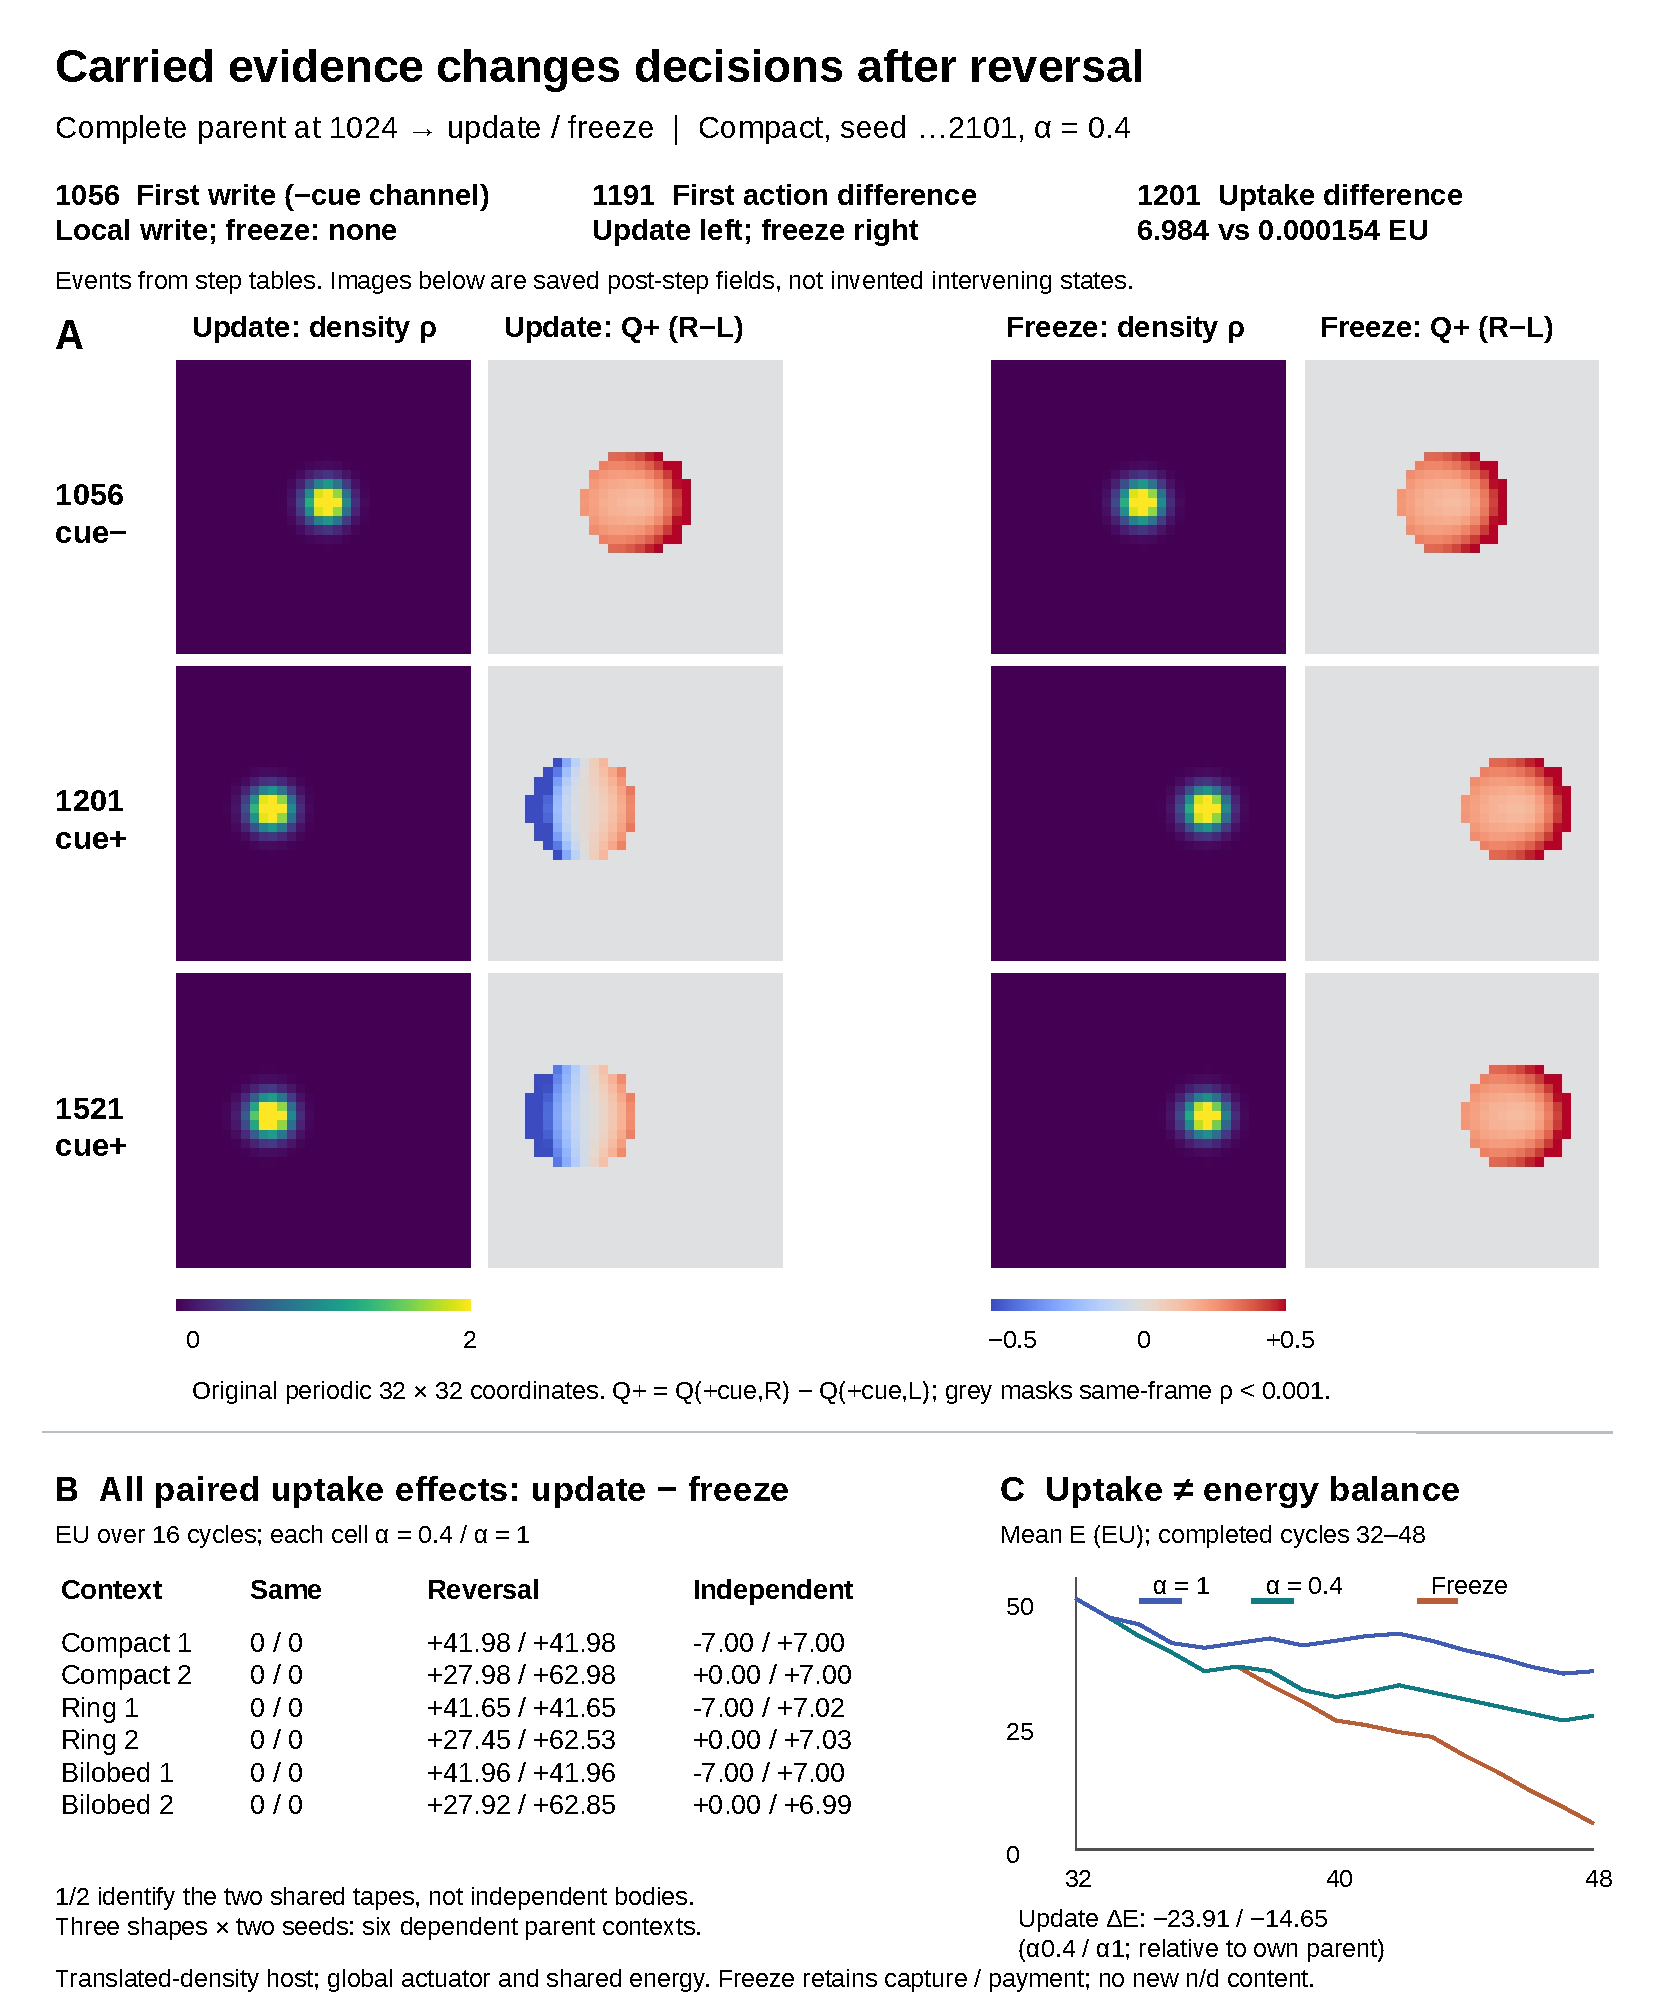
\includegraphics[width=\linewidth,height=0.79\textheight,keepaspectratio]{work/method_renewal/figures/carried_evidence/carried_evidence.pdf}
\captionsetup{font=footnotesize}
\caption{\textbf{Carried evidence changes action after a new reversal without restoring energy balance.}
A compact parent (seed 202610182101, $\alpha=0.4$) branches at step 1024. Logged differences first appear in negative-cue value writing at 1056, action at 1191 and uptake at 1201.
\textbf{a}, Actual saved density and positive-cue value contrast, $q_{+,R}-q_{+,L}$, at steps 1056, 1201 and 1521 for continued updating and paid freezing. Original $32\times32$ coordinates and common scales are retained. Grey masks density below $10^{-3}$; the saved fields lack denominator support, so the mask identifies tissue, not confidence. The first write concerns the negative-cue channel, whereas the stored contrast shows the positive-cue channel. No image at 1191 is inferred.
\textbf{b}, All six shape--seed paired uptake differences under unchanged, reversed and independent mappings, for both update rates. Shapes share two environmental tapes and are not independent histories.
\textbf{c}, Mean reversal-window energy. Updating improves energy relative to freezing, yet both update rates finish below their own parent energy. The faster rate $\alpha=1$ is a strong recent-feedback baseline. These persistent uptake-evidence fields are distinct from the disposable generation-choice channels tested in Table~\ref{tab:material-carried-choice}.}
\label{fig:carried-evidence}
\end{figure}


\subsection*{Actual local motor learning and content interventions}
The unified source is \path{local_motor_expression_20261019/direction_handoff.json}, SHA-256 \texttt{c5f6ce24\allowbreak{}a7e2fdc7\allowbreak{}f76a352f\allowbreak{}fcd84d69\allowbreak{}be9bbff6\allowbreak{}e1cb9666\allowbreak{}5eb39c71\allowbreak{}a5a1d299}. Its three archived reports, plans, full states, step tables and actual animations remain the primary records. Conditions 0 and 1 pair different seeds with opposite field signs; no cell-level or frame-level sample size is inferred. The first two capacity pilots are kept in the cost table but are not counted as extra learning histories. The manuscript's row transcription and per-step cost sums run no simulator or fit.

\begingroup\scriptsize\setlength{\tabcolsep}{3pt}\setlength{\LTpre}{6pt}\setlength{\LTpost}{6pt}
\begin{longtable}{llrrrrrrl}
\caption{All local-motor learning conditions. A/R/H denote acquisition, reversal and the unchanged-relation no-feedback phase. Scores and favourable fractions are means over each phase's final 64 updates. P/F reproduce the original conjunctive criterion.}\label{tab:motor-phases}\\
\toprule
Cond. & Rule & $S_A$ & $S_R$ & $S_H$ & $p_A$ & $p_R$ & $p_H$ & A/R/H \\
\midrule
\endfirsthead
\toprule
Cond. & Rule & $S_A$ & $S_R$ & $S_H$ & $p_A$ & $p_R$ & $p_H$ & A/R/H \\
\midrule
\endhead
0 & Fixed east & 0.46659 & 0.59933 & -0.71784 & 0.81513 & 0.88175 & 0.07641 & P/P/F \\
0 & Recipient immediate & 0.00911 & 0.18018 & 0.39094 & 0.41518 & 0.58708 & 0.79886 & F/F/P \\
0 & Recipient EMA & -0.01253 & 0.07220 & 0.12091 & 0.39303 & 0.47949 & 0.53096 & F/F/F \\
0 & Recipient EMA+neighbour & -0.01459 & 0.06694 & 0.10562 & 0.39110 & 0.47427 & 0.51492 & F/F/F \\
1 & Fixed east & -0.43844 & -0.57948 & 0.72025 & 0.20858 & 0.08954 & 0.91016 & F/F/P \\
1 & Recipient immediate & 0.07102 & -0.41816 & -0.60872 & 0.47630 & 0.05627 & 0.03327 & F/F/F \\
1 & Recipient EMA & 0.01405 & -0.02933 & -0.05577 & 0.41843 & 0.36507 & 0.33852 & F/F/F \\
1 & Recipient EMA+neighbour & 0.01156 & -0.01625 & -0.03672 & 0.41599 & 0.38262 & 0.36073 & F/F/F \\
0 & Source immediate & 0.72154 & -0.18610 & 0.01706 & 0.96399 & 0.39274 & 0.43269 & P/F/F \\
0 & Source EMA & 0.04634 & -0.08652 & -0.05384 & 0.45481 & 0.31534 & 0.34282 & F/F/F \\
0 & Source EMA+neighbour & 0.04328 & -0.09489 & -0.07410 & 0.45243 & 0.30485 & 0.32109 & F/F/F \\
1 & Source immediate & 0.74061 & -0.01191 & 0.44816 & 0.96661 & 0.41987 & 0.77952 & P/F/P \\
1 & Source EMA & 0.06593 & -0.12745 & -0.12081 & 0.47233 & 0.26311 & 0.27175 & F/F/F \\
1 & Source EMA+neighbour & 0.06418 & -0.11169 & -0.09521 & 0.47130 & 0.28477 & 0.30049 & F/F/F \\
\bottomrule
\end{longtable}
\begin{longtable}{lllrrrrrrr}
\caption{Actual whole-path energy and material accounts. Pilot rows have 256 updates; all learning rows have 896. Gain/loss are external paid consequences; motor and basal are physical expenditures. Unpaid requests and actual death remain separate. All rows end at mass 24 to displayed precision; no failed behavioural endpoint is removed.}\label{tab:motor-costs}\\
\toprule
Cond. & Stage & Rule & Gain & Loss & Motor & Basal & Unpaid & Death & End $E$ \\
\midrule
\endfirsthead
\toprule
Cond. & Stage & Rule & Gain & Loss & Motor & Basal & Unpaid & Death & End $E$ \\
\midrule
\endhead
0 & pilot & Fixed east & 20.10113 & 0.92264 & 0.92703 & 7.37280 & 0 & 0 & 154.87866 \\
1 & pilot & Fixed east & 0.93219 & 20.04536 & 0.92720 & 7.37280 & 0 & 0 & 116.58682 \\
0 & science & Fixed east & 45.87929 & 4.14604 & 3.25913 & 25.80480 & 0 & 0 & 156.66932 \\
0 & science & Recipient immediate & 13.87954 & 10.67440 & 2.50060 & 25.80480 & 0 & 0 & 118.89974 \\
0 & science & Recipient EMA & 12.64612 & 11.25300 & 2.48387 & 25.80480 & 0 & 0 & 117.10445 \\
0 & science & Recipient EMA+neighbour & 12.47860 & 11.17909 & 2.48570 & 25.80480 & 0 & 0 & 117.00901 \\
1 & science & Fixed east & 4.12776 & 45.88737 & 3.25763 & 25.80480 & 0 & 0 & 73.17796 \\
1 & science & Recipient immediate & 8.47034 & 18.38124 & 2.49494 & 25.80480 & 0 & 0 & 105.78936 \\
1 & science & Recipient EMA & 11.26358 & 12.09902 & 2.48125 & 25.80480 & 0 & 0 & 114.87851 \\
1 & science & Recipient EMA+neighbour & 11.49814 & 12.03074 & 2.48101 & 25.80480 & 0 & 0 & 115.18158 \\
0 & science & Source immediate & 18.19574 & 28.25958 & 2.82279 & 25.80480 & 0 & 0 & 105.30858 \\
0 & science & Source EMA & 10.73221 & 13.35536 & 2.48372 & 25.80480 & 0 & 0 & 113.08833 \\
0 & science & Source EMA+neighbour & 10.55892 & 13.31738 & 2.48499 & 25.80480 & 0 & 0 & 112.95175 \\
1 & science & Source immediate & 17.79108 & 27.47637 & 2.99284 & 25.80480 & 0 & 0 & 105.51706 \\
1 & science & Source EMA & 10.14200 & 13.64179 & 2.48420 & 25.80480 & 0 & 0 & 112.21122 \\
1 & science & Source EMA+neighbour & 10.41988 & 13.56453 & 2.48279 & 25.80480 & 0 & 0 & 112.56775 \\
\bottomrule
\end{longtable}
\begin{longtable}{llrrrrr}
\caption{All six 128-update expression futures from two complete step-320 parents. Displacement is signed along the original learned direction. Good/strong masses use $f>0$/$f>0.5$ and are time means, not endpoint masses. Every branch ends at mass 24 with zero external gain/loss. The expression step table omits separate basal and unpaid columns; these channels are not asserted to be measured zeros.}\label{tab:motor-expression}\\
\toprule
Parent & Content & Signed $\Delta x$ & Good $M$ & Strong $M$ & Motor & End $E$ \\
\midrule
\endfirsthead
\toprule
Parent & Content & Signed $\Delta x$ & Good $M$ & Strong $M$ & Motor & End $E$ \\
\midrule
\endhead
0 & retain & 4.30712 & 23.77062 & 23.15075 & 0.41466 & 141.95489 \\
0 & zero & -0.00182 & 23.58081 & 22.49769 & 0.35402 & 142.01553 \\
0 & negate & -4.42416 & 20.96045 & 15.85672 & 0.41382 & 141.95574 \\
1 & retain & 4.18421 & 23.80730 & 23.24000 & 0.41278 & 142.51433 \\
1 & zero & -0.00167 & 23.60146 & 22.58284 & 0.35143 & 142.57567 \\
1 & negate & -4.30046 & 21.35105 & 16.60726 & 0.41379 & 142.51331 \\
\bottomrule
\end{longtable}
\endgroup
\paragraph{Separate regenerative implementation.} The central joint-association comparison is archived at \path{src/environment_evolution/results/joint_behavior_actual_renewal_20261019/analysis/handoff.json}. Its original report retains four joint lives and their frozen-prior controls, actual rule deaths and paid births, pre-write bank copying, mass-floor truncations, full-window criteria, and the separate action-clamp diagnostic. Complete joint behaviour passes zero of four conditions. The diagnostic is explicitly clamped action, not learned reversal; its 16 stored steps are reused read-only. This source supports an architectural distinction from the local no-birth host, not a pooled estimate of learning or a newborn-content causal claim. The actual two-job record contains 4,035 new updates and 137.354014 worker seconds; no part was rerun for this manuscript.


\subsection*{Original finite ring physiology retained in full}
The complete earlier ring figure and its editable GUI source remain unchanged. It concerns a prescribed ring under a fixed generative rule, not the new density-regulated learning host in main Fig.~\ref{fig:young-turnover}.
\begin{figure}[p]
\centering
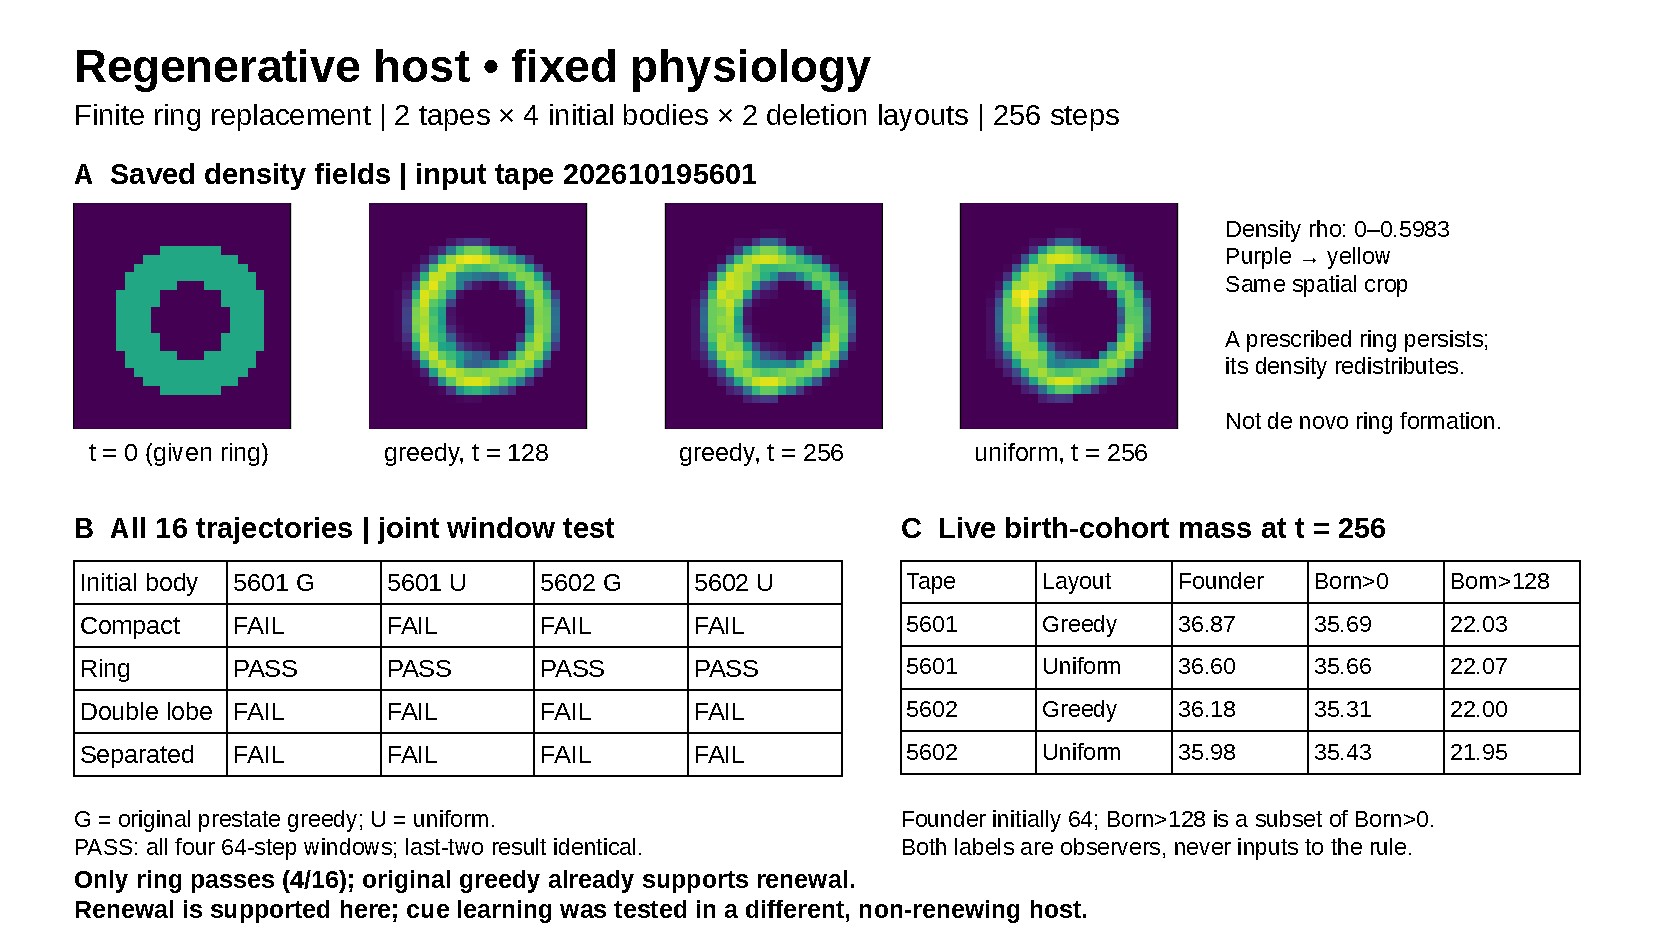
\includegraphics[width=\linewidth,height=.76\textheight,keepaspectratio]{work/longform_v047/figures/finite_replacement_v0474/finite_replacement.pdf}
\caption{\textbf{Finite replacement in a regenerative host under fixed physiology.}
\textbf{A}, Saved density fields for input tape 5601 show the prescribed initial ring and its continuation under original-greedy and uniform deletion layouts, with a common density scale and spatial crop. \textbf{B}, Two tapes, four initial shapes and two layouts give sixteen life-zero trajectories. Both ring seeds under both layouts pass all four fixed 64-step maintenance windows; the other twelve paths fail the final two-window criterion. \textbf{C}, Registered material amounts at step 256 distinguish retained founders from tissue born after life zero and after step 128. The latter is a subset of the former newborn category, not an additional disjoint cohort. Founders start at mass 64. The original rule already supports the ring result; uniform deletion coordination is not necessary. Initial rings are prescribed, not generated from compact starts. These regenerative bodies are distinct from the non-renewing cue-learning hosts in Figs.~\ref{fig:lifetime-learning} and \ref{fig:temporal-credit}; the experiments are not successive phases of one life. The finite 256-step result establishes neither a steady state nor learning, and additional deletion-coordination arithmetic is not physically priced.}
\label{fig:finite-replacement}
\end{figure}

\subsection*{Young density-regulated host: full energetic and newborn-content comparisons}
The synthesis source is \path{young_regenerative_learning_opportunity_20261019/synthesis/final_handoff.json}, read after the storage-summary correction as SHA-256 \texttt{062a874b\allowbreak{}d3108aa9\allowbreak{}bdce0c6d\allowbreak{}736cd92e\allowbreak{}7b39ff83\allowbreak{}6f405fcd\allowbreak{}fc42b8e6\allowbreak{}a6fa8b35}. The PI's model and storage correction is recorded in \path{knowledge_base/research/experience_learning/young_turnover_host_scientific_choice_20261019.json}. We retain the original six execution records and use the third and fifth recorded raw-file footprints (lower bounds on peak usage) explicitly, rather than repeating the outdated single-violation statement. The first bath trial supplies eight opportunity prefixes but no complete lives after expansion reaches the boundary. The bounded-habitat comparison and the direct-injury/content-reset comparisons remain in the original reports; they are not additional independent energetic-task replications. The complete source rows, including all auxiliary scalar charges, are registered in \path{work/longform_v047/data/young_turnover_source_rows_v0475.json}.

C/L denote compact/elongated initial geometry, 0/1 the opposite initial meanings. ``Prior'' never writes learned values; ``future freeze'' starts from the corresponding actual fast-256 state and therefore is not another life-zero acquisition. Probe rows inherit the same two acquired compact parents. No numerical terminal value is inserted for an unexecuted segment. The main-task later expression and newborn probe continue physical energetic outcomes while writing is off.
\begingroup\scriptsize\setlength{\tabcolsep}{3pt}\setlength{\LTpre}{6pt}\setlength{\LTpost}{6pt}
\begin{longtable}{lrrrrrrrrl}
\caption{All energetic-task paths and their original final-64 windows. A/R/H are acquisition, reversal and later stop-writing expression. Dashes denote unavailable or inapplicable windows, not measured failure. All four elongated main paths stop at 512; their planned terminal 128 updates are missing.}\label{tab:young-phases}\\
\toprule
Path & First & Last & $M_A$ & $M_R$ & $M_H$ & $p_A$ & $p_R$ & $p_H$ & A/R/H \\
\midrule\endfirsthead
\toprule
Path & First & Last & $M_A$ & $M_R$ & $M_H$ & $p_A$ & $p_R$ & $p_H$ & A/R/H \\
\midrule\endhead
C/0/fast & 1 & 640 & 75.1365 & 52.0639 & 80.1110 & 0.8163 & 0.4933 & 0.6381 & P/F/F \\
C/0/future freeze & 257 & 512 & -- & 27.7071 & -- & -- & 0.3082 & -- & --/F/-- \\
C/0/prior & 1 & 640 & 49.4568 & 50.7736 & 81.5577 & 0.5856 & 0.5141 & 0.6828 & F/F/P \\
C/1/fast & 1 & 640 & 68.9630 & 71.7772 & 100.0243 & 0.7621 & 0.6278 & 0.7310 & P/F/P \\
C/1/future freeze & 257 & 512 & -- & 26.5280 & -- & -- & 0.2910 & -- & --/F/-- \\
C/1/prior & 1 & 640 & 51.4448 & 58.9768 & 85.6635 & 0.6064 & 0.5722 & 0.6957 & F/F/P \\
L/0/fast & 1 & 512 & 47.6536 & 57.0086 & -- & 0.6185 & 0.5893 & -- & F/F/-- \\
L/0/future freeze & 257 & 512 & -- & 57.4187 & -- & -- & 0.5811 & -- & --/F/-- \\
L/0/prior & 1 & 512 & 47.7939 & 57.3109 & -- & 0.6286 & 0.6156 & -- & F/F/-- \\
L/1/fast & 1 & 512 & 44.8339 & 51.6136 & -- & 0.6100 & 0.5974 & -- & F/F/-- \\
L/1/future freeze & 257 & 512 & -- & 49.8584 & -- & -- & 0.6075 & -- & --/F/-- \\
L/1/prior & 1 & 512 & 43.8439 & 52.0777 & -- & 0.6077 & 0.6347 & -- & F/F/-- \\
\bottomrule
\end{longtable}
\begin{longtable}{lrrrrrrrrr}
\caption{Actual physical accounts for all twelve energetic paths and six newborn probes. Births and deaths are accumulated mass flows; post-birth fractions in other tables are retained stocks. External additions are actual $P/F$ injections, not a closed-reservoir exchange. Equal last clocks do not turn different parent histories into paired life-zero endpoints.}\label{tab:young-flows}\\
\toprule
Path & Steps & End $M$ & End $E$ & Birth & Rule death & Starvation & $P$ in & $F$ in & Uptake \\
\midrule\endfirsthead
\toprule
Path & Steps & End $M$ & End $E$ & Birth & Rule death & Starvation & $P$ in & $F$ in & Uptake \\
\midrule\endhead
C/0/fast & 640 & 138.0605 & 104.5608 & 521.1570 & 322.9244 & 131.4207 & 519.9477 & 862.1864 & 645.1866 \\
C/0/future freeze & 256 & 98.3380 & 36.6501 & 207.1724 & 128.6584 & 76.4374 & 206.9441 & 344.9497 & 258.0670 \\
C/0/prior & 640 & 132.8922 & 101.0390 & 498.0891 & 304.6322 & 131.8132 & 496.9129 & 817.0696 & 609.6923 \\
C/1/fast & 640 & 151.6715 & 129.5174 & 529.5700 & 333.7732 & 115.3739 & 528.3146 & 887.7298 & 667.3517 \\
C/1/future freeze & 256 & 105.1361 & 35.3437 & 216.1761 & 131.4770 & 73.6568 & 215.8993 & 354.2425 & 263.6839 \\
C/1/prior & 640 & 135.3066 & 104.7528 & 501.5338 & 310.9837 & 126.4921 & 500.3589 & 831.1504 & 622.3500 \\
L/0/fast & 512 & 116.0494 & 73.3464 & 351.1926 & 226.7996 & 79.5922 & 350.1776 & 593.8824 & 447.9663 \\
L/0/future freeze & 256 & 116.0101 & 72.3515 & 210.8694 & 128.3214 & 47.7930 & 210.5289 & 345.1531 & 257.1005 \\
L/0/prior & 512 & 105.9914 & 79.9154 & 326.8219 & 218.1854 & 73.8938 & 325.9368 & 563.4490 & 427.6140 \\
L/1/fast & 512 & 104.5545 & 68.7608 & 319.3274 & 212.5703 & 73.4512 & 318.4197 & 548.1486 & 415.4561 \\
L/1/future freeze & 256 & 104.1854 & 71.1904 & 184.9227 & 115.6509 & 40.5957 & 184.6057 & 308.8311 & 231.6456 \\
L/1/prior & 512 & 101.1334 & 71.6763 & 304.9441 & 208.1422 & 66.9171 & 304.0920 & 530.9940 & 404.2850 \\
C/0/copy & 128 & 113.2177 & 135.0046 & 94.5962 & 66.8811 & 10.7588 & 94.5149 & 168.6281 & 129.0873 \\
C/0/swap & 128 & 113.2177 & 135.0046 & 94.5962 & 66.8811 & 10.7588 & 94.5149 & 168.6281 & 129.0873 \\
C/0/zero & 128 & 113.2177 & 135.0046 & 94.5962 & 66.8811 & 10.7588 & 94.5149 & 168.6281 & 129.0873 \\
C/1/copy & 128 & 110.8432 & 123.0352 & 97.2242 & 65.2750 & 15.1999 & 97.1359 & 169.0406 & 128.3836 \\
C/1/swap & 128 & 109.1266 & 123.1508 & 95.4445 & 64.9114 & 15.5003 & 95.3796 & 166.4505 & 126.4954 \\
C/1/zero & 128 & 110.3445 & 123.7414 & 96.5560 & 65.1862 & 15.1190 & 96.4773 & 168.0672 & 127.6745 \\
\bottomrule
\end{longtable}
\begin{longtable}{lrrrrrrr}
\caption{Paid charges accumulated over each recorded path. Central computation, registrations and external-supply infrastructure are not priced. The two probe interventions retain the copying tariff; realized payments can diverge in later physical futures.}\label{tab:young-paid}\\
\toprule
Path & Motor & Basal & Copy & Hold & Tax & $P$ pump & $F$ pump \\
\midrule\endfirsthead
\toprule
Path & Motor & Basal & Copy & Hold & Tax & $P$ pump & $F$ pump \\
\midrule\endhead
C/0/fast & 84.2802 & 38.8298 & 0.6583 & 3.2332 & 419.4981 & 0.0000 & 0.0000 \\
C/0/future freeze & 19.8813 & 15.4849 & 0.2062 & 1.2893 & 278.0043 & 0.0000 & 0.0000 \\
C/0/prior & 83.9844 & 36.6350 & 0.6142 & 3.0327 & 413.4323 & 0.0000 & 0.0000 \\
C/1/fast & 98.5677 & 40.1220 & 0.7274 & 3.3371 & 386.9681 & 0.0000 & 0.0000 \\
C/1/future freeze & 33.5285 & 15.8214 & 0.2389 & 1.2976 & 265.4101 & 0.0000 & 0.0000 \\
C/1/prior & 88.8327 & 37.3939 & 0.6410 & 3.1157 & 409.1738 & 0.0000 & 0.0000 \\
L/0/fast & 73.0361 & 27.2637 & 0.4848 & 2.2589 & 305.7962 & 0.0000 & 0.0000 \\
L/0/future freeze & 36.1168 & 15.4272 & 0.2906 & 1.2700 & 176.4724 & 0.0000 & 0.0000 \\
L/0/prior & 47.4544 & 26.2266 & 0.4491 & 2.1776 & 296.6108 & 0.0000 & 0.0000 \\
L/1/fast & 60.7145 & 25.5525 & 0.4415 & 2.1193 & 291.8593 & 0.0000 & 0.0000 \\
L/1/future freeze & 33.7961 & 13.9025 & 0.2599 & 1.1508 & 152.3990 & 0.0000 & 0.0000 \\
L/1/prior & 55.0051 & 25.0172 & 0.4274 & 2.0766 & 278.3902 & 0.0000 & 0.0000 \\
C/0/copy & 11.4004 & 8.0322 & 0.1522 & 0.6693 & 17.7846 & 0.0000 & 0.0000 \\
C/0/swap & 11.4004 & 8.0322 & 0.1522 & 0.6693 & 17.7846 & 0.0000 & 0.0000 \\
C/0/zero & 11.4004 & 8.0322 & 0.1522 & 0.6693 & 17.7846 & 0.0000 & 0.0000 \\
C/1/copy & 14.3899 & 7.8421 & 0.1435 & 0.6535 & 25.7639 & 0.0000 & 0.0000 \\
C/1/swap & 10.3628 & 7.7987 & 0.1388 & 0.6499 & 26.8165 & 0.0000 & 0.0000 \\
C/1/zero & 12.3100 & 7.8314 & 0.1424 & 0.6526 & 25.8860 & 0.0000 & 0.0000 \\
\bottomrule
\end{longtable}
\begin{longtable}{lrrrrrr}
\caption{Unpaid or denied requests remain explicit, including small basal underpayments. A denied motor source request is distinct from an unpaid charge. These values are not converted to imaginary feedback or silently rounded to exact zero.}\label{tab:young-unpaid}\\
\toprule
Path & Motor unpaid & Motor denied & Basal unpaid & Copy denied & Hold denied & Tax unpaid \\
\midrule\endfirsthead
\toprule
Path & Motor unpaid & Motor denied & Basal unpaid & Copy denied & Hold denied & Tax unpaid \\
\midrule\endhead
C/0/fast & 0 & 15 & 2.47e-15 & 0.384 & 0.00262 & 189 \\
C/0/future freeze & 0 & 3.5 & 7.01e-16 & 0.208 & 0.00115 & 106 \\
C/0/prior & 0 & 12.3 & 2.44e-15 & 0.382 & 0.0203 & 187 \\
C/1/fast & 0 & 13.2 & 2.8e-15 & 0.332 & 0.00645 & 166 \\
C/1/future freeze & 0 & 7.07 & 9.9e-16 & 0.193 & 0.0209 & 103 \\
C/1/prior & 0 & 10.9 & 2.56e-15 & 0.362 & 0.000472 & 181 \\
L/0/fast & 0 & 11.1 & 1.99e-15 & 0.218 & 0.013 & 113 \\
L/0/future freeze & 0 & 5.7 & 1.03e-15 & 0.131 & 0.0156 & 67.4 \\
L/0/prior & 0 & 5.25 & 1.44e-15 & 0.205 & 0.00792 & 104 \\
L/1/fast & 0 & 6.99 & 1.7e-15 & 0.197 & 0.0101 & 102 \\
L/1/future freeze & 0 & 5.55 & 9.58e-16 & 0.11 & 0.00772 & 57.5 \\
L/1/prior & 0 & 7.83 & 1.59e-15 & 0.182 & 0.00818 & 95.6 \\
C/0/copy & 0 & 0.212 & 3.81e-16 & 0.037 & 0 & 15.3 \\
C/0/swap & 0 & 0.212 & 3.81e-16 & 0.037 & 0 & 15.3 \\
C/0/zero & 0 & 0.212 & 3.81e-16 & 0.037 & 0 & 15.3 \\
C/1/copy & 0 & 0.858 & 4.52e-16 & 0.051 & 0 & 21.4 \\
C/1/swap & 0 & 0.39 & 3.64e-16 & 0.0521 & 0 & 21.4 \\
C/1/zero & 0 & 0.649 & 4.06e-16 & 0.0507 & 0 & 21.1 \\
\bottomrule
\end{longtable}
\begin{longtable}{lrrrrr}
\caption{All six matched-parent newborn-content probes. Safe contact is absolute mass; the following columns are contact fraction and retained tissue fractions born since 256 or life zero. They are not one-to-one founder replacement. The last column is the measured content load of the last newborn cohort. All probes pass finite expression while physical feedback remains present.}\label{tab:young-payload}\\
\toprule
Parent/content & Safe $M$ & Safe share & Born $>256$ & Born $>0$ & Newborn load \\
\midrule\endfirsthead
\toprule
Parent/content & Safe $M$ & Safe share & Born $>256$ & Born $>0$ & Newborn load \\
\midrule\endhead
C/0/copy & 94.1804 & 0.8837 & 0.5880 & 0.9292 & 0.5568 \\
C/0/swap & 94.1804 & 0.8837 & 0.5880 & 0.9292 & 0.4992 \\
C/0/zero & 94.1804 & 0.8837 & 0.5880 & 0.9292 & 0.0000 \\
C/1/copy & 86.7266 & 0.8324 & 0.6047 & 0.9333 & 0.5159 \\
C/1/swap & 85.5179 & 0.8258 & 0.5993 & 0.9324 & 0.4347 \\
C/1/zero & 86.6058 & 0.8333 & 0.6027 & 0.9330 & 0.0000 \\
\bottomrule
\end{longtable}
\begin{longtable}{lrrrrrrr}
\caption{Conversion and loss accounts over each recorded path. Birth fuel $F_B=0.42B$ is partitioned into newborn energy $E_B=0.20B$, synthesis heat $H_s=0.20B$ and template heat $H_t=0.02B$; the partition is not an additional expense on top of $F_B$. Total heat change includes the heat components and all other paid dissipation. Dead energy is energy carried by removed tissue. All 18 complete energy accounts close within $1.14\times10^{-13}$.}\label{tab:young-conversion}\\
\toprule
Path & $F_B$ & $E_B$ & $H_s$ & $H_t$ & $\Delta H$ & $\Delta E_d$ & $\Delta W$ \\
\midrule\endfirsthead
\toprule
Path & $F_B$ & $E_B$ & $H_s$ & $H_t$ & $\Delta H$ & $\Delta E_d$ & $\Delta W$ \\
\midrule\endhead
C/0/fast & 218.8860 & 104.2314 & 104.2314 & 10.4231 & 661.1541 & 226.6052 & 454.3451 \\
C/0/future freeze & 87.0124 & 41.4345 & 41.4345 & 4.1434 & 360.4440 & 50.2663 & 205.0958 \\
C/0/prior & 209.1974 & 99.6178 & 99.6178 & 9.9618 & 647.2781 & 198.8201 & 436.4455 \\
C/1/fast & 222.4194 & 105.9140 & 105.9140 & 10.5914 & 646.2277 & 242.2735 & 449.1471 \\
C/1/future freeze & 90.7940 & 43.2352 & 43.2352 & 4.3235 & 363.8552 & 47.0756 & 205.1338 \\
C/1/prior & 210.6442 & 100.3068 & 100.3068 & 10.0307 & 649.4945 & 206.9944 & 437.4759 \\
L/0/fast & 147.5009 & 70.2385 & 70.2385 & 7.0239 & 486.1022 & 164.2661 & 306.3918 \\
L/0/future freeze & 88.5651 & 42.1739 & 42.1739 & 4.2174 & 275.9683 & 66.4144 & 176.1143 \\
L/0/prior & 137.2652 & 65.3644 & 65.3644 & 6.5364 & 444.8193 & 168.3920 & 292.0791 \\
L/1/fast & 134.1175 & 63.8655 & 63.8655 & 6.3865 & 450.9392 & 158.1211 & 286.0215 \\
L/1/future freeze & 77.6675 & 36.9845 & 36.9845 & 3.6985 & 242.1913 & 62.8067 & 156.2466 \\
L/1/prior & 128.0765 & 60.9888 & 60.9888 & 6.0989 & 428.0042 & 160.9286 & 275.0594 \\
C/0/copy & 39.7304 & 18.9192 & 18.9192 & 1.8919 & 58.8498 & 77.2443 & 77.6399 \\
C/0/swap & 39.7304 & 18.9192 & 18.9192 & 1.8919 & 58.8498 & 77.2443 & 77.6399 \\
C/0/zero & 39.7304 & 18.9192 & 18.9192 & 1.8919 & 58.8498 & 77.2443 & 77.6399 \\
C/1/copy & 40.8342 & 19.4448 & 19.4448 & 1.9445 & 70.1822 & 67.7970 & 80.4749 \\
C/1/swap & 40.0867 & 19.0889 & 19.0889 & 1.9089 & 66.7645 & 68.4634 & 80.4117 \\
C/1/zero & 40.5535 & 19.3112 & 19.3112 & 1.9311 & 68.0648 & 68.2184 & 80.3053 \\
\bottomrule
\end{longtable}
\begin{longtable}{lrrrrrrrr}
\caption{Initial body and energy, endpoint extracellular and dissipated stocks, and body-time. Future-freeze and newborn rows inherit nonzero physical inventories from their actual parent. Endpoint heat, dead energy and waste are cumulative stocks; Table~\ref{tab:young-conversion} reports changes over the branch only. All initial and final inventories, including inherited $P/F$, heat, dead energy and waste, are indexed by the exact path key in the additional-accounts source JSON.}\label{tab:young-inventories}\\
\toprule
Path & Start $M$ & Start $E$ & End $P$ & End $F$ & End $H$ & End $E_d$ & End $W$ & Body-time \\
\midrule\endfirsthead
\toprule
Path & Start $M$ & Start $E$ & End $P$ & End $F$ & End $H$ & End $E_d$ & End $W$ & Body-time \\
\midrule\endhead
C/0/fast & 71.2486 & 128.2475 & 817.9906 & 817.3138 & 661.1541 & 226.6052 & 454.3451 & 3239.1557 \\
C/0/future freeze & 96.2614 & 102.2810 & 818.2634 & 817.8241 & 545.9745 & 172.4655 & 335.2831 & 1290.5098 \\
C/0/prior & 71.2486 & 128.2475 & 818.0238 & 817.3798 & 647.2781 & 198.8201 & 436.4455 & 3055.9952 \\
C/1/fast & 71.2486 & 128.2475 & 817.9446 & 817.1587 & 646.2277 & 242.2735 & 449.1471 & 3347.5220 \\
C/1/future freeze & 94.0938 & 91.7966 & 818.2125 & 817.7349 & 570.1757 & 158.6045 & 339.0264 & 1319.0053 \\
C/1/prior & 71.2486 & 128.2475 & 818.0251 & 817.3562 & 649.4945 & 206.9944 & 437.4759 & 3119.3647 \\
L/0/fast & 71.2486 & 128.2475 & 818.1851 & 817.6152 & 486.1022 & 164.2661 & 306.3918 & 2274.2158 \\
L/0/future freeze & 81.2550 & 69.0686 & 818.1977 & 817.6208 & 485.5742 & 165.7969 & 305.2791 & 1287.3412 \\
L/0/prior & 71.2486 & 128.2475 & 818.3149 & 817.7697 & 444.8193 & 168.3920 & 292.0791 & 2187.2854 \\
L/1/fast & 71.2486 & 128.2475 & 818.2923 & 817.7750 & 450.9392 & 158.1211 & 286.0215 & 2131.0412 \\
L/1/future freeze & 75.5093 & 66.8753 & 818.3066 & 817.7847 & 444.2770 & 160.6308 & 283.4169 & 1159.9726 \\
L/1/prior & 71.2486 & 128.2475 & 818.3479 & 817.8325 & 428.0042 & 160.9286 & 275.0594 & 2086.2625 \\
C/0/copy & 96.2614 & 102.2810 & 818.4104 & 817.7641 & 244.3803 & 199.4436 & 207.8272 & 670.1964 \\
C/0/swap & 96.2614 & 102.2810 & 818.4104 & 817.7641 & 244.3803 & 199.4436 & 207.8272 & 670.1964 \\
C/0/zero & 96.2614 & 102.2810 & 818.4104 & 817.7641 & 244.3803 & 199.4436 & 207.8272 & 670.1964 \\
C/1/copy & 94.0938 & 91.7966 & 818.4010 & 817.7931 & 276.5027 & 179.3259 & 214.3674 & 654.3471 \\
C/1/swap & 94.0938 & 91.7966 & 818.4244 & 817.8388 & 273.0850 & 179.9923 & 214.3043 & 650.6408 \\
C/1/zero & 94.0938 & 91.7966 & 818.4107 & 817.8095 & 274.3853 & 179.7473 & 214.1978 & 653.4309 \\
\bottomrule
\end{longtable}
\endgroup


\subsection*{Earlier acquired motor-bias intervention retained in full}
The earlier local-bias figure remains unchanged below, with all original source-credit, EMA and recipient comparisons, two actual parents and six no-feedback interventions. Its acquisition $2/2$ and reversal $0/2$ result is not revised by the subsequent gain policy in Supplementary Fig.~\ref{fig:acquired-gain}. A GUI-reconstructed editable counterpart is supplied as \path{figures/local_motor_v0475/recovered_editable/local_motor_reconstructed.pptx} within the working manuscript directory. It preserves the native text and vector geometry and eight cropped actual fields, with minor layout differences documented in the accompanying reconstruction record. The original PDF export is retained here; the reconstructed PPTX has a new hash and is not a recovery of the unavailable original bytes.
\begin{figure}[p]
\centering
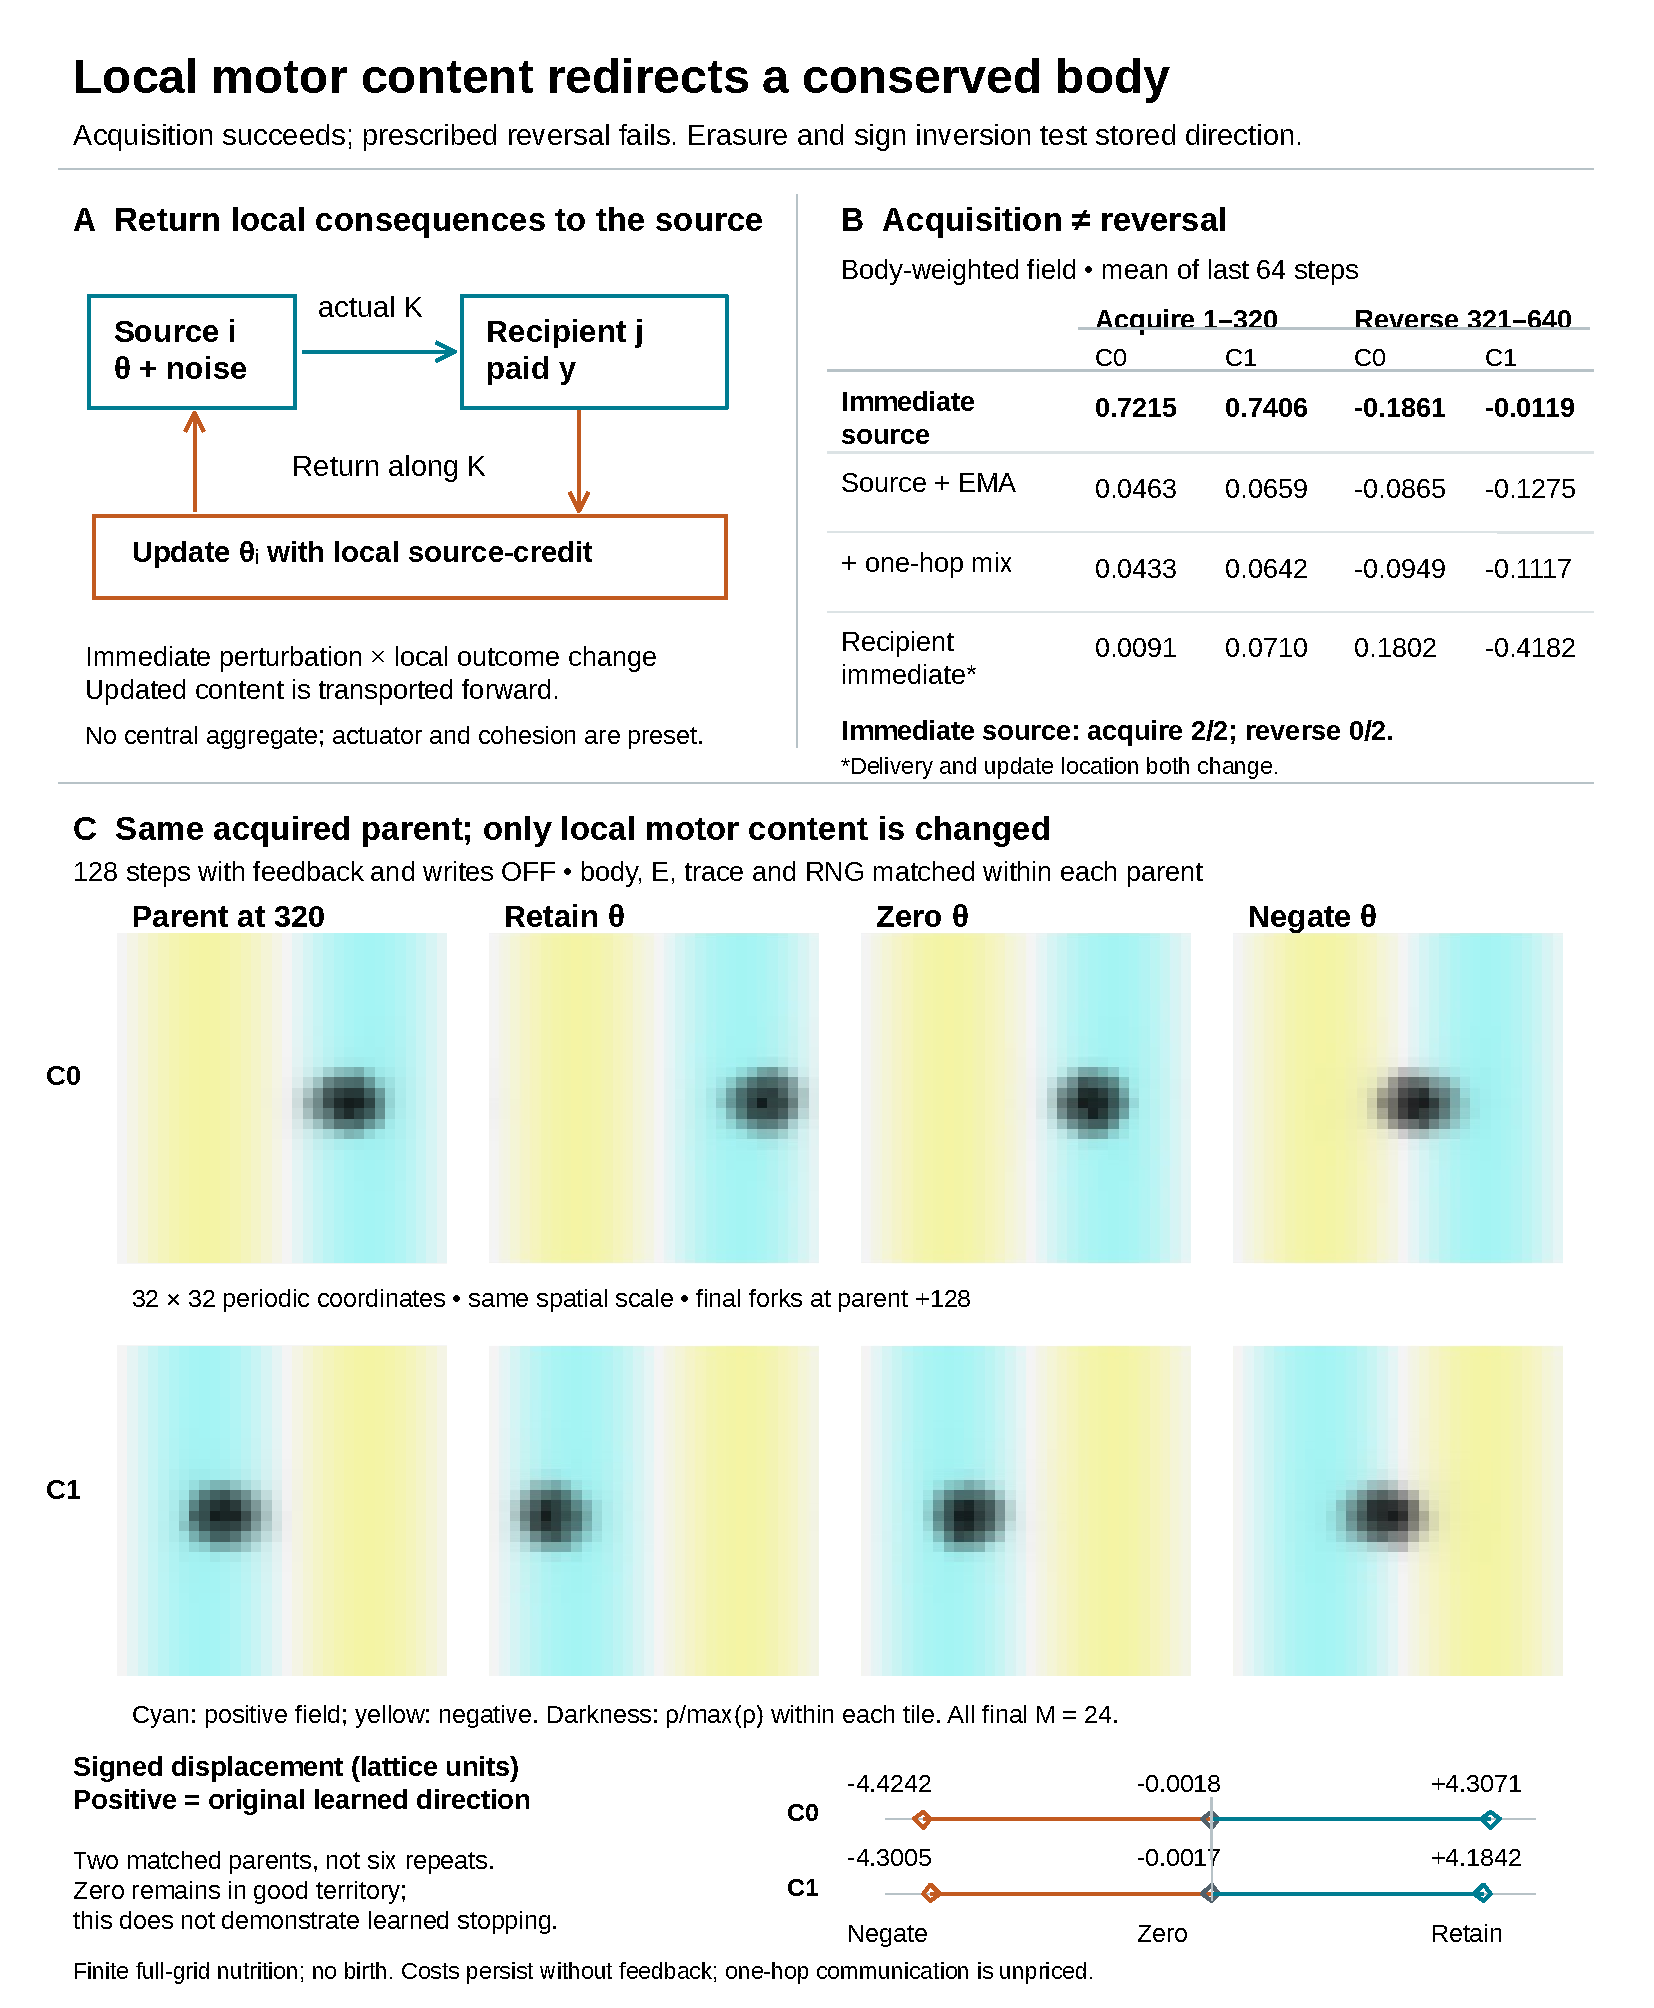
\includegraphics[width=\linewidth,height=0.69\textheight,keepaspectratio]{work/longform_v047/figures/local_motor_v0475/local_motor.pdf}
\captionsetup{font=footnotesize}
\caption{\textbf{Acquired local motor content affects action without successful reversal.}
\textbf{a}, Actually paid local consequences return along executed transport edges to the motor source; updated content travels forward with material. The stochastic actuator and cohesion are supplied, with no central action or reward aggregation. Source and recipient comparisons change both feedback delivery and writing location.
\textbf{b}, The two seed--field conditions acquire a directional bias with the standard immediate source-credit rule but fail the prescribed environmental reversal. Scores are final-64 tissue-weighted field means, not accuracy; the original criterion also requires favourable mass fraction and viability. Tested EMA and neighbour variants do not establish an advantage, and their effective gains are not matched to the immediate rule.
\textbf{c}, Each complete actual-320 parent branches into retained, zeroed and sign-reversed motor content for 128 updates with no payment or new writing. Actual fields retain original coordinates; cyan/yellow denote positive/negative field. Darkness is normalized within each density tile, not a shared absolute-density scale. Signed displacement is measured along each parent's original learned direction. All six futures remain mass 24; zeroed branches retain favourable occupancy and pay less for motion, so almost zero net displacement does not imply learned stopping. These are paired interventions in two parents, not six independent histories. This no-birth local host is distinct from the density-regulated central-action host in Fig.~\ref{fig:young-turnover}; extra one-hop communication and learning arithmetic are unpriced.}
\label{fig:local-motor-content}
\end{figure}

\subsection*{State-dependent action and acquired response gain}
The four source batches are indexed by \path{acquired_gain_content_20261019/direction_handoff.json}, SHA-256 \texttt{5045d649\allowbreak{}75466cb1\allowbreak{}1c69e28f\allowbreak{}332fdccb\allowbreak{}a2962188\allowbreak{}385fbbe6\allowbreak{}2a2141b4\allowbreak{}324c087a}. Batches 1--4 respectively test linear state readout, unchanged-relation controls from actual parents, a scalar conditional gain and its acquired content. They comprise 18,816 actual updates and 118.121236 worker seconds, with no unknown updates or replay of old acquisition or futures. There are fourteen life-zero paths and eighteen dependent continuations, not 32 independent lives. The manuscript's transcription and cost aggregation run no model or fit. All failed original gates and all costs are retained.
\begingroup\scriptsize\setlength{\tabcolsep}{3pt}\setlength{\LTpre}{6pt}\setlength{\LTpost}{6pt}

\begin{longtable}{rlllrrrrl}
\caption{All 78 recorded phase windows. B identifies the batch; C identifies the paired seed--field condition. A/R/H are acquisition, changed-relation feedback and no-new-feedback aftereffect; U is the unchanged-relation control. $S$ and $p_+$ are final-64 body-weighted field score and favourable-half mass fraction. P/F are the original conjunctive occupancy and viability gates, not retrospective judgements about relearning. Blank acquisition windows are never invented for forks.}\label{tab:gain-phases}\\
\toprule
B/C & Rule & Phase & $S$ & $p_+$ & $M_{end}$ & $E_{end}$ & Paid gain & Gate \\
\midrule
\endfirsthead
\toprule
B/C & Rule & Phase & $S$ & $p_+$ & $M_{end}$ & $E_{end}$ & Paid gain & Gate \\
\midrule
\endhead
1/0 & Bias & A & 0.71704 & 0.96168 & 24.00000 & 146.13781 & 15.09757 & P \\
1/0 & Bias & R & -0.56467 & 0.13823 & 24.00000 & 105.93567 & 1.00106 & F \\
1/0 & Bias & H & -0.04471 & 0.50861 & 24.00000 & 101.82958 & 0.00000 & F \\
1/0 & Linear & A & 0.71993 & 0.96244 & 24.00000 & 146.20120 & 15.15352 & P \\
1/0 & Linear & R & -0.56549 & 0.13949 & 24.00000 & 106.00113 & 1.01480 & F \\
1/0 & Linear & H & -0.05111 & 0.50278 & 24.00000 & 101.89517 & 0.00000 & F \\
1/0 & Filtered & A & 0.72424 & 0.97646 & 24.00000 & 150.56720 & 18.59305 & P \\
1/0 & Filtered & R & -0.10059 & 0.34239 & 24.00000 & 123.65226 & 1.94128 & F \\
1/0 & Filtered & H & 0.29883 & 0.71843 & 24.00000 & 119.59148 & 0.00000 & P \\
1/0 & Linear frozen & R & -0.12369 & 0.47462 & 24.00000 & 112.41100 & 1.05874 & F \\
1/0 & Linear frozen & H & 0.56428 & 0.94934 & 24.00000 & 108.30971 & 0.00000 & P \\
1/0 & Bias readout & R & -0.12862 & 0.46956 & 24.00000 & 112.34071 & 1.03325 & F \\
1/0 & Bias readout & H & 0.55762 & 0.94832 & 24.00000 & 108.24018 & 0.00000 & P \\
1/1 & Bias & A & 0.74041 & 0.96529 & 24.00000 & 146.61649 & 15.57477 & P \\
1/1 & Bias & R & 0.31804 & 0.70794 & 24.00000 & 119.56176 & 4.14629 & P \\
1/1 & Bias & H & 0.75108 & 0.92655 & 24.00000 & 115.38254 & 0.00000 & P \\
1/1 & Linear & A & 0.74315 & 0.96594 & 24.00000 & 146.67919 & 15.62999 & P \\
1/1 & Linear & R & 0.32329 & 0.71176 & 24.00000 & 119.72165 & 4.19775 & P \\
1/1 & Linear & H & 0.75089 & 0.92674 & 24.00000 & 115.54208 & 0.00000 & P \\
1/1 & Filtered & A & 0.73127 & 0.97730 & 24.00000 & 150.68099 & 18.69981 & P \\
1/1 & Filtered & R & -0.14480 & 0.30071 & 24.00000 & 122.65290 & 1.72616 & F \\
1/1 & Filtered & H & 0.25695 & 0.67934 & 24.00000 & 118.59553 & 0.00000 & P \\
1/1 & Linear frozen & R & -0.06777 & 0.35750 & 24.00000 & 114.02290 & 1.29589 & F \\
1/1 & Linear frozen & H & 0.60224 & 0.91874 & 24.00000 & 109.92392 & 0.00000 & P \\
1/1 & Bias readout & R & -0.07302 & 0.35187 & 24.00000 & 113.94581 & 1.26621 & F \\
1/1 & Bias readout & H & 0.59564 & 0.91631 & 24.00000 & 109.84752 & 0.00000 & P \\
2/0 & Bias & U & 0.44552 & 0.89898 & 24.00000 & 163.23396 & 27.40377 & P \\
2/0 & Bias & H & 0.33445 & 0.79769 & 24.00000 & 159.18496 & 0.00000 & P \\
2/0 & Linear & U & 0.45471 & 0.90758 & 24.00000 & 163.41275 & 27.51345 & P \\
2/0 & Linear & H & 0.35823 & 0.82380 & 24.00000 & 159.36397 & 0.00000 & P \\
2/0 & Filtered & U & 0.93149 & 0.99421 & 24.00000 & 174.23712 & 33.99490 & P \\
2/0 & Filtered & H & 0.94483 & 0.99635 & 24.00000 & 170.19225 & 0.00000 & P \\
2/0 & Linear frozen & U & 0.13353 & 0.53529 & 24.00000 & 159.64015 & 24.69300 & F \\
2/0 & Linear frozen & H & -0.55086 & 0.05257 & 24.00000 & 155.54040 & 0.00000 & F \\
2/1 & Bias & U & 0.45367 & 0.98885 & 24.00000 & 163.48520 & 27.16943 & P \\
2/1 & Bias & H & 0.39116 & 0.97401 & 24.00000 & 159.43862 & 0.00000 & P \\
2/1 & Linear & U & 0.46402 & 0.99094 & 24.00000 & 163.67790 & 27.29378 & P \\
2/1 & Linear & H & 0.41470 & 0.98229 & 24.00000 & 159.63142 & 0.00000 & P \\
2/1 & Filtered & U & 0.93279 & 0.99446 & 24.00000 & 174.58478 & 34.21995 & P \\
2/1 & Filtered & H & 0.94557 & 0.99661 & 24.00000 & 170.53824 & 0.00000 & P \\
2/1 & Linear frozen & U & 0.07826 & 0.65348 & 24.00000 & 158.99297 & 23.79900 & F \\
2/1 & Linear frozen & H & -0.58896 & 0.08603 & 24.00000 & 154.89538 & 0.00000 & F \\
3/0 & Bias & A & 0.72791 & 0.96278 & 24.00000 & 146.59665 & 15.53046 & P \\
3/0 & Bias & R & -0.79875 & 0.06707 & 24.00000 & 103.88366 & 0.80332 & F \\
3/0 & Bias & H & -0.73068 & 0.08065 & 24.00000 & 99.83892 & 0.00000 & F \\
3/0 & Learned gain & A & 0.73116 & 0.96284 & 24.00000 & 146.62755 & 15.55933 & P \\
3/0 & Learned gain & R & 0.34187 & 0.66910 & 24.00000 & 128.12180 & 8.89882 & P \\
3/0 & Learned gain & H & 0.57144 & 0.82715 & 24.00000 & 123.97599 & 0.00000 & P \\
3/0 & Fixed gain & A & 0.97833 & 0.99937 & 24.00000 & 162.13878 & 29.37527 & P \\
3/0 & Fixed gain & R & 0.74831 & 0.96551 & 24.00000 & 148.50805 & 10.24677 & P \\
3/0 & Fixed gain & H & 0.96891 & 0.99884 & 24.00000 & 144.35124 & 0.00000 & P \\
3/0 & Zero gain & A & 0.01973 & 0.42894 & 24.00000 & 134.45720 & 6.40723 & F \\
3/0 & Zero gain & R & -0.01247 & 0.39180 & 24.00000 & 123.87701 & 5.40105 & F \\
3/0 & Zero gain & H & -0.02260 & 0.37422 & 24.00000 & 119.83935 & 0.00000 & F \\
3/0 & Gain frozen & R & 0.56962 & 0.89553 & 24.00000 & 132.94564 & 8.56271 & P \\
3/0 & Gain frozen & H & 0.88502 & 0.98828 & 24.00000 & 128.84137 & 0.00000 & P \\
3/1 & Bias & A & 0.71766 & 0.95951 & 24.00000 & 146.17913 & 15.21598 & P \\
3/1 & Bias & R & 0.01491 & 0.47123 & 24.00000 & 116.07552 & 3.88639 & F \\
3/1 & Bias & H & 0.36327 & 0.69535 & 24.00000 & 111.90938 & 0.00000 & P \\
3/1 & Learned gain & A & 0.72261 & 0.95975 & 24.00000 & 146.23304 & 15.26912 & P \\
3/1 & Learned gain & R & 0.76330 & 0.91537 & 24.00000 & 137.88629 & 13.06424 & P \\
3/1 & Learned gain & H & 0.78826 & 0.97910 & 24.00000 & 133.70735 & 0.00000 & P \\
3/1 & Fixed gain & A & 0.97800 & 0.99941 & 24.00000 & 162.03007 & 29.28525 & P \\
3/1 & Fixed gain & R & 0.75103 & 0.95374 & 24.00000 & 148.51673 & 10.30808 & P \\
3/1 & Fixed gain & H & 0.96606 & 0.99827 & 24.00000 & 144.34748 & 0.00000 & P \\
3/1 & Zero gain & A & -0.00647 & 0.39908 & 24.00000 & 133.75192 & 6.07223 & F \\
3/1 & Zero gain & R & 0.00977 & 0.41076 & 24.00000 & 124.11899 & 5.93320 & F \\
3/1 & Zero gain & H & 0.02082 & 0.42436 & 24.00000 & 120.07954 & 0.00000 & F \\
3/1 & Gain frozen & R & 0.61387 & 0.90213 & 24.00000 & 133.98361 & 9.28632 & P \\
3/1 & Gain frozen & H & 0.88362 & 0.98697 & 24.00000 & 129.87737 & 0.00000 & P \\
4/0 & Erase & R & -0.82935 & 0.01489 & 24.00000 & 104.66589 & 0.26247 & F \\
4/0 & Erase & H & -0.82263 & 0.01542 & 24.00000 & 100.62500 & 0.00000 & F \\
4/0 & Uniform & R & 0.57261 & 0.90334 & 24.00000 & 132.90200 & 8.43687 & P \\
4/0 & Uniform & H & 0.89549 & 0.99188 & 24.00000 & 128.79788 & 0.00000 & P \\
4/1 & Erase & R & -0.81331 & 0.01386 & 24.00000 & 104.83085 & 0.26100 & F \\
4/1 & Erase & H & -0.81299 & 0.01491 & 24.00000 & 100.79105 & 0.00000 & F \\
4/1 & Uniform & R & 0.61592 & 0.91079 & 24.00000 & 133.89256 & 9.13349 & P \\
4/1 & Uniform & H & 0.89470 & 0.99129 & 24.00000 & 129.78627 & 0.00000 & P \\
\bottomrule
\end{longtable}

\begin{longtable}{rlllrrr}
\caption{Phase-specific actual expenditure for every window in the preceding table. These are whole-phase sums, not final-64 sums. External gain/loss and motor expenditure are distinct; complete basal and unpaid accounts are in the path table.}\label{tab:gain-phase-costs}\\
\toprule
B/C & Rule & Phase & Updates & Gain & Loss & Motor \\
\midrule
\endfirsthead
\toprule
B/C & Rule & Phase & Updates & Gain & Loss & Motor \\
\midrule
\endhead
1/0 & Bias & A & 320 & 15.09757 & 2.80478 & 0.93898 \\
1/0 & Bias & R & 320 & 1.00106 & 30.99907 & 0.98813 \\
1/0 & Bias & H & 128 & 0.00000 & 0.00000 & 0.41969 \\
1/0 & Linear & A & 320 & 15.15352 & 2.79681 & 0.93951 \\
1/0 & Linear & R & 320 & 1.01480 & 31.01182 & 0.98705 \\
1/0 & Linear & H & 128 & 0.00000 & 0.00000 & 0.41956 \\
1/0 & Filtered & A & 320 & 18.59305 & 1.88430 & 0.92555 \\
1/0 & Filtered & R & 320 & 1.94128 & 18.73142 & 0.90880 \\
1/0 & Filtered & H & 128 & 0.00000 & 0.00000 & 0.37438 \\
1/0 & Linear frozen & R & 320 & 1.05874 & 24.60159 & 1.03134 \\
1/0 & Linear frozen & H & 128 & 0.00000 & 0.00000 & 0.41489 \\
1/0 & Bias readout & R & 320 & 1.03325 & 24.64713 & 1.03061 \\
1/0 & Bias readout & H & 128 & 0.00000 & 0.00000 & 0.41412 \\
1/1 & Bias & A & 320 & 15.57477 & 2.79712 & 0.94516 \\
1/1 & Bias & R & 320 & 4.14629 & 20.84193 & 1.14308 \\
1/1 & Bias & H & 128 & 0.00000 & 0.00000 & 0.49282 \\
1/1 & Linear & A & 320 & 15.62999 & 2.78910 & 0.94570 \\
1/1 & Linear & R & 320 & 4.19775 & 20.79570 & 1.14360 \\
1/1 & Linear & H & 128 & 0.00000 & 0.00000 & 0.49316 \\
1/1 & Filtered & A & 320 & 18.69981 & 1.87647 & 0.92634 \\
1/1 & Filtered & R & 320 & 1.72616 & 19.63175 & 0.90650 \\
1/1 & Filtered & H & 128 & 0.00000 & 0.00000 & 0.37097 \\
1/1 & Linear frozen & R & 320 & 1.29589 & 23.70235 & 1.03382 \\
1/1 & Linear frozen & H & 128 & 0.00000 & 0.00000 & 0.41259 \\
1/1 & Bias readout & R & 320 & 1.26621 & 23.75055 & 1.03304 \\
1/1 & Bias readout & H & 128 & 0.00000 & 0.00000 & 0.41189 \\
2/0 & Bias & U & 320 & 27.40377 & 0.08976 & 1.00186 \\
2/0 & Bias & H & 128 & 0.00000 & 0.00000 & 0.36260 \\
2/0 & Linear & U & 320 & 27.51345 & 0.08544 & 1.00046 \\
2/0 & Linear & H & 128 & 0.00000 & 0.00000 & 0.36238 \\
2/0 & Filtered & U & 320 & 33.99490 & 0.18804 & 0.92094 \\
2/0 & Filtered & H & 128 & 0.00000 & 0.00000 & 0.35847 \\
2/0 & Linear frozen & U & 320 & 24.69300 & 1.00816 & 1.02989 \\
2/0 & Linear frozen & H & 128 & 0.00000 & 0.00000 & 0.41335 \\
2/1 & Bias & U & 320 & 27.16943 & 0.09077 & 0.99394 \\
2/1 & Bias & H & 128 & 0.00000 & 0.00000 & 0.36018 \\
2/1 & Linear & U & 320 & 27.29378 & 0.08638 & 0.99268 \\
2/1 & Linear & H & 128 & 0.00000 & 0.00000 & 0.36008 \\
2/1 & Filtered & U & 320 & 34.21995 & 0.18353 & 0.91663 \\
2/1 & Filtered & H & 128 & 0.00000 & 0.00000 & 0.36014 \\
2/1 & Linear frozen & U & 320 & 23.79900 & 1.23694 & 1.03227 \\
2/1 & Linear frozen & H & 128 & 0.00000 & 0.00000 & 0.41119 \\
3/0 & Bias & A & 320 & 15.53046 & 2.77592 & 0.94189 \\
3/0 & Bias & R & 320 & 0.80332 & 33.37659 & 0.92372 \\
3/0 & Bias & H & 128 & 0.00000 & 0.00000 & 0.35834 \\
3/0 & Learned gain & A & 320 & 15.55933 & 2.77211 & 0.94367 \\
3/0 & Learned gain & R & 320 & 8.89882 & 17.14350 & 1.04508 \\
3/0 & Learned gain & H & 128 & 0.00000 & 0.00000 & 0.45941 \\
3/0 & Fixed gain & A & 320 & 29.37527 & 0.83818 & 1.18231 \\
3/0 & Fixed gain & R & 320 & 10.24677 & 13.50124 & 1.16026 \\
3/0 & Fixed gain & H & 128 & 0.00000 & 0.00000 & 0.47041 \\
3/0 & Zero gain & A & 320 & 6.40723 & 5.85228 & 0.88175 \\
3/0 & Zero gain & R & 320 & 5.40105 & 5.87744 & 0.88780 \\
3/0 & Zero gain & H & 128 & 0.00000 & 0.00000 & 0.35126 \\
3/0 & Gain frozen & R & 320 & 8.56271 & 12.00061 & 1.02802 \\
3/0 & Gain frozen & H & 128 & 0.00000 & 0.00000 & 0.41786 \\
3/1 & Bias & A & 320 & 15.21598 & 2.87814 & 0.94272 \\
3/1 & Bias & R & 320 & 3.88639 & 23.65558 & 1.11841 \\
3/1 & Bias & H & 128 & 0.00000 & 0.00000 & 0.47974 \\
3/1 & Learned gain & A & 320 & 15.26912 & 2.87533 & 0.94474 \\
3/1 & Learned gain & R & 320 & 13.06424 & 11.06622 & 1.12878 \\
3/1 & Learned gain & H & 128 & 0.00000 & 0.00000 & 0.49254 \\
3/1 & Fixed gain & A & 320 & 29.28525 & 0.84440 & 1.19479 \\
3/1 & Fixed gain & R & 320 & 10.30808 & 13.44646 & 1.15896 \\
3/1 & Fixed gain & H & 128 & 0.00000 & 0.00000 & 0.48284 \\
3/1 & Zero gain & A & 320 & 6.07223 & 6.21703 & 0.88729 \\
3/1 & Zero gain & R & 320 & 5.93320 & 5.46636 & 0.88377 \\
3/1 & Zero gain & H & 128 & 0.00000 & 0.00000 & 0.35305 \\
3/1 & Gain frozen & R & 320 & 9.28632 & 11.28519 & 1.03457 \\
3/1 & Gain frozen & H & 128 & 0.00000 & 0.00000 & 0.41983 \\
4/0 & Erase & R & 320 & 0.26247 & 32.11851 & 0.88963 \\
4/0 & Erase & H & 128 & 0.00000 & 0.00000 & 0.35449 \\
4/0 & Uniform & R & 320 & 8.43687 & 11.91791 & 1.02851 \\
4/0 & Uniform & H & 128 & 0.00000 & 0.00000 & 0.41771 \\
4/1 & Erase & R & 320 & 0.26100 & 31.55425 & 0.89295 \\
4/1 & Erase & H & 128 & 0.00000 & 0.00000 & 0.35340 \\
4/1 & Uniform & R & 320 & 9.13349 & 11.22326 & 1.03471 \\
4/1 & Uniform & H & 128 & 0.00000 & 0.00000 & 0.41989 \\
\bottomrule
\end{longtable}

\begin{longtable}{rllrrrrrrr}
\caption{Complete physical energy accounts for all 32 actual paths. The start column prevents a 448-update fork from being mistaken for a new acquired life. $E_0$ is read from its actual saved starting state. All terms are measured in the implemented physical energy units; additional arithmetic, storage and communication have no assigned physical tariff.}\label{tab:gain-costs}\\
\toprule
B/C & Rule & Start & $E_0$ & $E_{end}$ & Gain & Loss & Motor & Basal & Unpaid \\
\midrule
\endfirsthead
\toprule
B/C & Rule & Start & $E_0$ & $E_{end}$ & Gain & Loss & Motor & Basal & Unpaid \\
\midrule
\endhead
1/0 & Bias & 0 & 144.00000 & 101.82958 & 16.09863 & 33.80385 & 2.34680 & 22.11840 & 0.00000 \\
1/0 & Linear & 0 & 144.00000 & 101.89517 & 16.16831 & 33.80862 & 2.34611 & 22.11840 & 0.00000 \\
1/0 & Filtered & 0 & 144.00000 & 119.59148 & 20.53433 & 20.61572 & 2.20873 & 22.11840 & 0.00000 \\
1/0 & Linear frozen & 320 & 146.20120 & 108.30971 & 1.05874 & 24.60159 & 1.44623 & 12.90240 & 0.00000 \\
1/0 & Bias readout & 320 & 146.20120 & 108.24018 & 1.03325 & 24.64713 & 1.44473 & 12.90240 & 0.00000 \\
1/1 & Bias & 0 & 144.00000 & 115.38254 & 19.72106 & 23.63905 & 2.58107 & 22.11840 & 0.00000 \\
1/1 & Linear & 0 & 144.00000 & 115.54208 & 19.82774 & 23.58480 & 2.58246 & 22.11840 & 0.00000 \\
1/1 & Filtered & 0 & 144.00000 & 118.59553 & 20.42597 & 21.50823 & 2.20381 & 22.11840 & 0.00000 \\
1/1 & Linear frozen & 320 & 146.67919 & 109.92392 & 1.29589 & 23.70235 & 1.44641 & 12.90240 & 0.00000 \\
1/1 & Bias readout & 320 & 146.67919 & 109.84752 & 1.26621 & 23.75055 & 1.44493 & 12.90240 & 0.00000 \\
2/0 & Bias & 320 & 146.13781 & 159.18496 & 27.40377 & 0.08976 & 1.36446 & 12.90240 & 0.00000 \\
2/0 & Linear & 320 & 146.20120 & 159.36397 & 27.51345 & 0.08544 & 1.36284 & 12.90240 & 0.00000 \\
2/0 & Filtered & 320 & 150.56720 & 170.19225 & 33.99490 & 0.18804 & 1.27942 & 12.90240 & 0.00000 \\
2/0 & Linear frozen & 320 & 146.20120 & 155.54040 & 24.69300 & 1.00816 & 1.44324 & 12.90240 & 0.00000 \\
2/1 & Bias & 320 & 146.61649 & 159.43862 & 27.16943 & 0.09077 & 1.35413 & 12.90240 & 0.00000 \\
2/1 & Linear & 320 & 146.67919 & 159.63142 & 27.29378 & 0.08638 & 1.35276 & 12.90240 & 0.00000 \\
2/1 & Filtered & 320 & 150.68099 & 170.53824 & 34.21995 & 0.18353 & 1.27678 & 12.90240 & 0.00000 \\
2/1 & Linear frozen & 320 & 146.67919 & 154.89538 & 23.79900 & 1.23694 & 1.44347 & 12.90240 & 0.00000 \\
3/0 & Bias & 0 & 144.00000 & 99.83892 & 16.33379 & 36.15251 & 2.22396 & 22.11840 & 0.00000 \\
3/0 & Learned gain & 0 & 144.00000 & 123.97599 & 24.45816 & 19.91561 & 2.44816 & 22.11840 & 0.00000 \\
3/0 & Fixed gain & 0 & 144.00000 & 144.35124 & 39.62204 & 14.33942 & 2.81298 & 22.11840 & 0.00000 \\
3/0 & Zero gain & 0 & 144.00000 & 119.83935 & 11.80828 & 11.72972 & 2.12081 & 22.11840 & 0.00000 \\
3/0 & Gain frozen & 320 & 146.62755 & 128.84137 & 8.56271 & 12.00061 & 1.44588 & 12.90240 & 0.00000 \\
3/1 & Bias & 0 & 144.00000 & 111.90938 & 19.10237 & 26.53373 & 2.54086 & 22.11840 & 0.00000 \\
3/1 & Learned gain & 0 & 144.00000 & 133.70735 & 28.33336 & 13.94155 & 2.56605 & 22.11840 & 0.00000 \\
3/1 & Fixed gain & 0 & 144.00000 & 144.34748 & 39.59333 & 14.29086 & 2.83660 & 22.11840 & 0.00000 \\
3/1 & Zero gain & 0 & 144.00000 & 120.07954 & 12.00543 & 11.68338 & 2.12411 & 22.11840 & 0.00000 \\
3/1 & Gain frozen & 320 & 146.23304 & 129.87737 & 9.28632 & 11.28519 & 1.45440 & 12.90240 & 0.00000 \\
4/0 & Erase & 320 & 146.62755 & 100.62500 & 0.26247 & 32.11851 & 1.24412 & 12.90240 & 0.00000 \\
4/0 & Uniform & 320 & 146.62755 & 128.79788 & 8.43687 & 11.91791 & 1.44623 & 12.90240 & 0.00000 \\
4/1 & Erase & 320 & 146.23304 & 100.79105 & 0.26100 & 31.55425 & 1.24635 & 12.90240 & 0.00000 \\
4/1 & Uniform & 320 & 146.23304 & 129.78627 & 9.13349 & 11.22326 & 1.45460 & 12.90240 & 0.00000 \\
\bottomrule
\end{longtable}

\begin{longtable}{rllrrrrrrr}
\caption{Material and energy checks on the same actual paths. No births occur. Actual death is tabulated rather than inferred from a rounded endpoint. Body-time is $0.1\sum_t M_t$ over the recorded updates. The last column is the absolute whole-path energy residual $|E_{end}-E_0-G+L+C_{motor}+C_{basal}|$; no additional cost is inferred from an absent tariff.}\label{tab:gain-material}\\
\toprule
B/C & Rule & Updates & $M_0$ & $M_{end}$ & $M_{min}$ & Min. conn. & Death & Body-time & Residual \\
\midrule
\endfirsthead
\toprule
B/C & Rule & Updates & $M_0$ & $M_{end}$ & $M_{min}$ & Min. conn. & Death & Body-time & Residual \\
\midrule
\endhead
1/0 & Bias & 768 & 24.00000 & 24.00000 & 24.00000 & 0.99317 & 0.00000 & 1843.20000 & 2.1e-14 \\
1/0 & Linear & 768 & 24.00000 & 24.00000 & 24.00000 & 0.99371 & 0.00000 & 1843.20000 & 1.8e-14 \\
1/0 & Filtered & 768 & 24.00000 & 24.00000 & 24.00000 & 0.99266 & 0.00000 & 1843.20000 & 1.1e-14 \\
1/0 & Linear frozen & 448 & 24.00000 & 24.00000 & 24.00000 & 0.99359 & 0.00000 & 1075.20000 & 1.6e-14 \\
1/0 & Bias readout & 448 & 24.00000 & 24.00000 & 24.00000 & 0.99356 & 0.00000 & 1075.20000 & 3.7e-14 \\
1/1 & Bias & 768 & 24.00000 & 24.00000 & 24.00000 & 0.99395 & 0.00000 & 1843.20000 & 0.0e+00 \\
1/1 & Linear & 768 & 24.00000 & 24.00000 & 24.00000 & 0.99394 & 0.00000 & 1843.20000 & 8.9e-14 \\
1/1 & Filtered & 768 & 24.00000 & 24.00000 & 24.00000 & 0.99302 & 0.00000 & 1843.20000 & 1.4e-14 \\
1/1 & Linear frozen & 448 & 24.00000 & 24.00000 & 24.00000 & 0.99348 & 0.00000 & 1075.20000 & 1.8e-15 \\
1/1 & Bias readout & 448 & 24.00000 & 24.00000 & 24.00000 & 0.99360 & 0.00000 & 1075.20000 & 5.7e-14 \\
2/0 & Bias & 448 & 24.00000 & 24.00000 & 24.00000 & 0.99373 & 0.00000 & 1075.20000 & 1.8e-15 \\
2/0 & Linear & 448 & 24.00000 & 24.00000 & 24.00000 & 0.99376 & 0.00000 & 1075.20000 & 3.6e-14 \\
2/0 & Filtered & 448 & 24.00000 & 24.00000 & 24.00000 & 0.99168 & 0.00000 & 1075.20000 & 7.1e-14 \\
2/0 & Linear frozen & 448 & 24.00000 & 24.00000 & 24.00000 & 0.99357 & 0.00000 & 1075.20000 & 3.6e-14 \\
2/1 & Bias & 448 & 24.00000 & 24.00000 & 24.00000 & 0.99381 & 0.00000 & 1075.20000 & 8.9e-15 \\
2/1 & Linear & 448 & 24.00000 & 24.00000 & 24.00000 & 0.99378 & 0.00000 & 1075.20000 & 3.4e-14 \\
2/1 & Filtered & 448 & 24.00000 & 24.00000 & 24.00000 & 0.99159 & 0.00000 & 1075.20000 & 4.3e-14 \\
2/1 & Linear frozen & 448 & 24.00000 & 24.00000 & 24.00000 & 0.99360 & 0.00000 & 1075.20000 & 7.1e-15 \\
3/0 & Bias & 768 & 24.00000 & 24.00000 & 24.00000 & 0.98844 & 0.00000 & 1843.20000 & 3.6e-15 \\
3/0 & Learned gain & 768 & 24.00000 & 24.00000 & 24.00000 & 0.99410 & 0.00000 & 1843.20000 & 5.7e-14 \\
3/0 & Fixed gain & 768 & 24.00000 & 24.00000 & 24.00000 & 0.99568 & 0.00000 & 1843.20000 & 5.3e-14 \\
3/0 & Zero gain & 768 & 24.00000 & 24.00000 & 24.00000 & 0.99133 & 0.00000 & 1843.20000 & 4.6e-14 \\
3/0 & Gain frozen & 448 & 24.00000 & 24.00000 & 24.00000 & 0.98524 & 0.00000 & 1075.20000 & 5.7e-14 \\
3/1 & Bias & 768 & 24.00000 & 24.00000 & 24.00000 & 0.99462 & 0.00000 & 1843.20000 & 6.4e-14 \\
3/1 & Learned gain & 768 & 24.00000 & 24.00000 & 24.00000 & 0.99238 & 0.00000 & 1843.20000 & 1.4e-14 \\
3/1 & Fixed gain & 768 & 24.00000 & 24.00000 & 24.00000 & 0.99525 & 0.00000 & 1843.20000 & 8.2e-14 \\
3/1 & Zero gain & 768 & 24.00000 & 24.00000 & 24.00000 & 0.99163 & 0.00000 & 1843.20000 & 0.0e+00 \\
3/1 & Gain frozen & 448 & 24.00000 & 24.00000 & 24.00000 & 0.98106 & 0.00000 & 1075.20000 & 4.8e-14 \\
4/0 & Erase & 448 & 24.00000 & 24.00000 & 24.00000 & 0.99135 & 0.00000 & 1075.20000 & 2.7e-14 \\
4/0 & Uniform & 448 & 24.00000 & 24.00000 & 24.00000 & 0.97938 & 0.00000 & 1075.20000 & 6.4e-14 \\
4/1 & Erase & 448 & 24.00000 & 24.00000 & 24.00000 & 0.99119 & 0.00000 & 1075.20000 & 2.5e-14 \\
4/1 & Uniform & 448 & 24.00000 & 24.00000 & 24.00000 & 0.97117 & 0.00000 & 1075.20000 & 5.7e-14 \\
\bottomrule
\end{longtable}

\begin{longtable}{rllrrrrr}
\caption{Matched actual-320 relation controls. Displacement is along the original learned direction over the entire 448-step continuation, whereas command is a final-64 mean and field/good mass are terminal values. The first eight consecutive opposite-direction commands are reported by their final clock, when present. Every pair has exactly equal first mean command, sampled motor and transport operator; later full physical futures can diverge.}\label{tab:gain-relation}\\
\toprule
C & Rule & Relation & $\Delta x$ & Command & $S_{end}$ & $M_{+,end}$ & First 8 \\
\midrule
\endfirsthead
\toprule
C & Rule & Relation & $\Delta x$ & Command & $S_{end}$ & $M_{+,end}$ & First 8 \\
\midrule
\endhead
0 & Bias & changed & 10.84681 & 0.61242 & 0.07503 & 14.53769 & -- \\
0 & Bias & unchanged & 8.50649 & 0.08363 & 0.30771 & 18.33784 & -- \\
0 & Linear & changed & 10.75915 & 0.60725 & 0.06686 & 14.34493 & -- \\
0 & Linear & unchanged & 8.32455 & 0.07153 & 0.33504 & 19.08275 & -- \\
0 & Filtered & changed & -7.30811 & -0.32939 & 0.38990 & 19.15264 & 330 \\
0 & Filtered & unchanged & 2.56591 & 0.06352 & 0.94596 & 23.92099 & -- \\
0 & Linear frozen & changed & 14.71950 & 0.65981 & 0.69544 & 23.38969 & -- \\
0 & Linear frozen & unchanged & 14.59756 & 0.65035 & -0.68340 & 0.60917 & -- \\
1 & Bias & changed & 20.18241 & 1.14592 & 0.68591 & 21.49769 & -- \\
1 & Bias & unchanged & 7.87071 & 0.04605 & 0.36740 & 23.01881 & -- \\
1 & Linear & changed & 20.20543 & 1.14764 & 0.68368 & 21.48259 & -- \\
1 & Linear & unchanged & 7.68557 & 0.03431 & 0.39467 & 23.31771 & -- \\
1 & Filtered & changed & -7.20440 & -0.32684 & 0.35394 & 18.43217 & 330 \\
1 & Filtered & unchanged & 2.48514 & 0.06268 & 0.94542 & 23.92718 & -- \\
1 & Linear frozen & changed & 14.69449 & 0.65922 & 0.72568 & 23.14236 & -- \\
1 & Linear frozen & unchanged & 14.56932 & 0.64977 & -0.71416 & 0.88322 & -- \\
\bottomrule
\end{longtable}

\begin{longtable}{rllrr}
\caption{Actual-320 gain-content interventions, two parents with dependent forks. The four new interventions preserve body, energy, non-gain auxiliary fields, memory, eligibility and random-generator state exactly at branching. Homogenization preserves the parent mass-weighted scalar gain but not each vector command or nonlinear motor amplitude. Global averaging occurs only in the experimental intervention. The retained/frozen reference was recorded in batch 3 and reused read-only.}\label{tab:gain-parent}\\
\toprule
C & Intervention & Other fields/RNG & $\bar\kappa_0$ & Max. initial command change \\
\midrule
\endfirsthead
\toprule
C & Intervention & Other fields/RNG & $\bar\kappa_0$ & Max. initial command change \\
\midrule
\endhead
0 & Erase & identical & 0.66305 & 0.87275 \\
0 & Uniform & identical & 0.66305 & 0.58363 \\
1 & Erase & identical & 0.67034 & 0.87973 \\
1 & Uniform & identical & 0.67034 & 0.58656 \\
\bottomrule
\end{longtable}

\endgroup


\subsection*{Information-rich action comparisons retained in full}\label{supp:information-rich-action}
The following earlier action analysis and its original gain figure are preserved with their supplied directional information. The primary scalar experiment in the main text uses a stricter observation interface.
\subsection*{Acquired local motor content changes the body's subsequent direction}

The preceding cue assays supply either cue-gradient actuation or a common readout of local evidence. A separate experiment asks whether experience can instead establish a bodily movement bias when action and its update remain local. A deformable material body starts with zero two-component motor parameters on a periodic $32\times32$ lattice. Each occupied location perturbs its own motor drive; only actually completed local energy gains and losses provide feedback. The policy receives no global position, field map, hidden outcome sign or reversal clock, and no body-wide action or reward is pooled. Cohesion, pressure, motor axes and the stochastic actuator are preinstalled. Nutritional consequences cover the entire finite substrate, so this is not the sparse recontact problem above. This conservative host has no tissue birth (Supplementary Fig.~\ref{fig:local-motor-content}).

The implementation comparison concerns where the consequence of a local movement is used. In the recipient-credit variant, transported perturbation scores are combined with the paid result at the receiving location. In the source-credit variant, the paid result is returned along the executed transport edges to the location that generated the perturbation; the resulting parameter update is then transported forward with the material. Thus the latter changes both feedback delivery and the site of writing. It is not a clean comparison of optimizers, nor does it identify a unique mediator. The score-based immediate update is a standard simple rule; no new algorithm is inferred from this routing choice.

Two paired seed--field conditions use opposite initial outcome signs. Under source-credit immediate updates, the acquisition-window mean tissue-weighted field scores are $0.72154$ and $0.74061$, with favourable-half mass fractions $0.96399$ and $0.96661$. Both satisfy the original acquisition criterion, whereas the corresponding recipient-immediate cases do not. The two conditions combine different noise/body seeds with opposite fields; they are not a factorial demonstration of generalization across bodies. An exponentially averaged score and an additional occupied-neighbour averaging step fail acquisition in both tested conditions. Their nominal learning rate is shared with the immediate rule, but the normalized exponential average reduces the current perturbation's effective gain. These unoptimized settings do not establish a general inferiority of eligibility traces. The preset eastward control can also obtain positive scores periodically and is retained as an action-capacity control with a directional prior (Supplementary Tables~\ref{tab:motor-phases} and \ref{tab:motor-costs}).

Acquisition is followed by failure to reverse. The actual outcome sign changes at step 321, with paid feedback available immediately. Neither source-immediate path passes the prescribed reversal window: its final-64 mean scores are $-0.18610$ and $-0.01191$, and neither reaches the recorded 32-step recovery criterion during that phase. Only one later no-feedback endpoint passes, giving no complete acquire--reverse--retain life. All six source-credit lives remain viable at mass 24. The failure therefore concerns behavioural revision under the registered opportunities, not material extinction. Continued movement and positive acquisition alone cannot establish adaptation to changed consequences.

We then intervene on the acquired content rather than comparing two already divergent histories. Each complete source-immediate parent at actual step 320 supplies three 128-update futures with payments and new writes disabled. Body, energy, sensory registers, trace and random-generator state are identical within each parent; only the two motor-parameter fields are retained, set to zero or sign-reversed at the branch. Physical dynamics, local exploration and real material transport continue. Along the original learned direction, the two retained branches move $4.3071$ and $4.1842$ lattice units; zeroed branches move $-0.00182$ and $-0.00167$; sign-reversed branches move $-4.4242$ and $-4.3005$. The actual spatial fields and paired displacement distinguish content-dependent action from a difference in initial placement (Supplementary Fig.~\ref{fig:local-motor-content}). Six futures remain two paired parent interventions, not six independent replicates.

The intervention also shows why displacement and useful occupancy must be separated. The zeroed bodies remain in previously acquired favourable locations and pay less for movement: $0.3540$ and $0.3514$, versus $0.4147$ and $0.4128$ with retained parameters. Mean mass in the strongly favourable region is still $22.4977$ and $22.5828$ after zeroing, compared with $23.1507$ and $23.2400$ under retention. These are absolute amounts within bodies of mass 24, not ratios rescued by tiny contact. Their occupancy does not imply learned stopping. Conversely, sign reversal changes the entire subsequent physical future; its effect is not a mediation percentage or a measure of relearning without feedback. Full endpoint energy, occupancy and costs are retained in Supplementary Table~\ref{tab:motor-expression}.

This local, non-renewing host must also be distinguished from the separate regenerative joint-association implementation. That implementation combines a central five-action readout with actual paid births, rule deaths and copying from local pre-write banks. Its four joint lives do not pass the complete behavioural sequence; compact histories can stop at the registered mass floor, while fragmented histories can retain preferences without passing the absolute-contact requirements. The local motor-content intervention here neither supplies that central controller nor tests newborn content. Actual renewal in one implementation and causal motor expression in another do not establish that local learning survives replacement in the same body. The present positive result is narrower and actionable: experience-acquired local content affects whole-body motion, while this acquired-bias implementation fails to revise its direction appropriately after new consequences.

\subsection*{Acquired response gain is sufficient for feedback-triggered turning, but reversal need not require relearning}

The directional-bias result leaves two possibilities: the body may need a new way to update its policy, or it may need to express acquired content conditionally on what it currently senses. We examine that distinction while retaining local execution, actual transport, paid feedback and the no-birth host. In all four new batches, behaviour is scored over the last 64 updates of the prescribed phase using the same field and favourable-mass criteria. These scores describe occupancy. They do not, by themselves, identify how the body arrived there or whether it revised an acquired response.

A linear policy first adds two state-dependent terms to the learned bias, using the previous actual paid-outcome gradient as input. This change does not establish an additional capability. The mass-weighted magnitudes of the two state terms at acquisition are only $0.00246$ and $0.00229$, compared with a bias near $0.656$; the conditional and bias-only paths are nearly coincident. In one condition, both pass the original complete occupancy criterion while continuing mainly in the old direction around the periodic domain. We preserve that passing gate, but do not interpret it as learning to turn (Supplementary Table~\ref{tab:gain-phases}).

An unchanged-relation control from the same complete acquired state explains the ambiguity. Freezing the linear weights leaves the two bodies moving along their original direction whether the payment relation changes or stays unchanged. Their respective 448-update signed displacements are $14.7195/14.5976$ and $14.6945/14.5693$ lattice units under changed/unchanged relations. The nearly same route ends in a favourable region after the change and an unfavourable region without it. At the first continuation update the mean commands, sampled motors and actual transport operators match exactly within all eight pairs. Later payments also change energy and the physical future, so this comparison is not a pure policy-mediation estimate. It nevertheless shows why a favourable endpoint under reversal is insufficient evidence of relearning. The supplied fixed gradient-feedback control actually reverses its command after new feedback, despite failing the earlier prescribed reversal endpoint (Supplementary Table~\ref{tab:gain-relation}).

We next remove the accumulating additive bias and use a standard one-parameter conditional Gaussian policy. The mean command is $\boldsymbol\mu=\kappa\boldsymbol d$, where $\boldsymbol d$ is the unit direction of the last legally observed local paid-outcome gradient and the learned scalar $\kappa$ starts at zero. Local perturbations and their returned consequences update the response gain; transport carries the updated quantity with the material. Gradient direction, Cartesian motor axes and their interpretation as movement remain supplied. This experiment tests acquisition of a usable response strength, not discovery of a sensory direction or a new optimizer (Fig.~\ref{fig:acquired-gain}).

In two new seed--field conditions, both learned-gain lives pass acquisition, reversal and the no-new-feedback aftereffect in the same uninterrupted trajectory. Their phase scores are $0.73116/0.34187/0.57144$ and $0.72261/0.76330/0.78826$. The bias-only and zero-gain controls each have zero complete successes. However, a fixed positive-gain controller, $\kappa=1$, also passes both complete sequences and is a strong alternative: its corresponding scores are $0.97833/0.74831/0.96891$ and $0.97800/0.75103/0.96606$. Thus the new representation enables a conditional capability, but no advantage over the supplied simple direction-following rule is established. This result does not change the earlier immediate-bias experiment's acquisition $2/2$ and reversal $0/2$ outcomes.

The causal role of acquired gain is narrower than the aggregate phase result. From each actual learned body at step 320, we stop only gain writing while retaining real sensing, material transport and physical feedback. Both continuations still pass reversal and aftereffect. The first changed payment arrives at step 321, after that step's action; the updated legal gradient can alter the next command at step 322. Existing gain combined with new sensory evidence is therefore sufficient for the tested change of direction. Successful behaviour after a hidden reversal does not demonstrate that the gain had to be learned again.

Content interventions identify what remains necessary in these two acquired parents. Clearing only $\kappa$ while continuing to freeze its writes makes both reversal and aftereffect fail: their scores are $-0.82935/-0.82263$ and $-0.81331/-0.81299$. Replacing the spatial gain field by its original body-mass-weighted mean succeeds in both parents, with scores $0.57261/0.89549$ and $0.61592/0.89470$, close to the retained/frozen references $0.56962/0.88502$ and $0.61387/0.88362$. The acquired scalar content is usable, whereas its particular heterogeneous distribution is not required in these continuations. These are two matched parents with dependent futures. Erasure changes the drive immediately, and homogenization matches the scalar mean rather than every nonlinear action; neither intervention identifies a unique mediator or a matched-drive effect (Supplementary Table~\ref{tab:gain-parent}).

All 32 recorded paths survive with mass approximately 24, including the failed behavioural conditions and dependent branches. The learned-gain lives end with energies $123.976$ and $133.707$ and spend $2.44816$ and $2.56605$ on movement; the fixed-gain controls end at $144.351$ and $144.347$ while spending $2.81298$ and $2.83660$. Greater movement cost can accompany stronger occupancy and higher energy, so no simultaneous-improvement requirement is imposed. All phase outcomes, payments, basal costs and physical checks remain in Supplementary Tables~\ref{tab:gain-phases}--\ref{tab:gain-material}. During the final 128 updates there are no new payments or new reward-gradient observations: previously lawful records are transported and read. This finite aftereffect does not establish sustained current sensing, general adaptation, or learning maintained through tissue renewal. The latter remains a separate question in the regenerative host.

\begin{figure}[p]
\centering
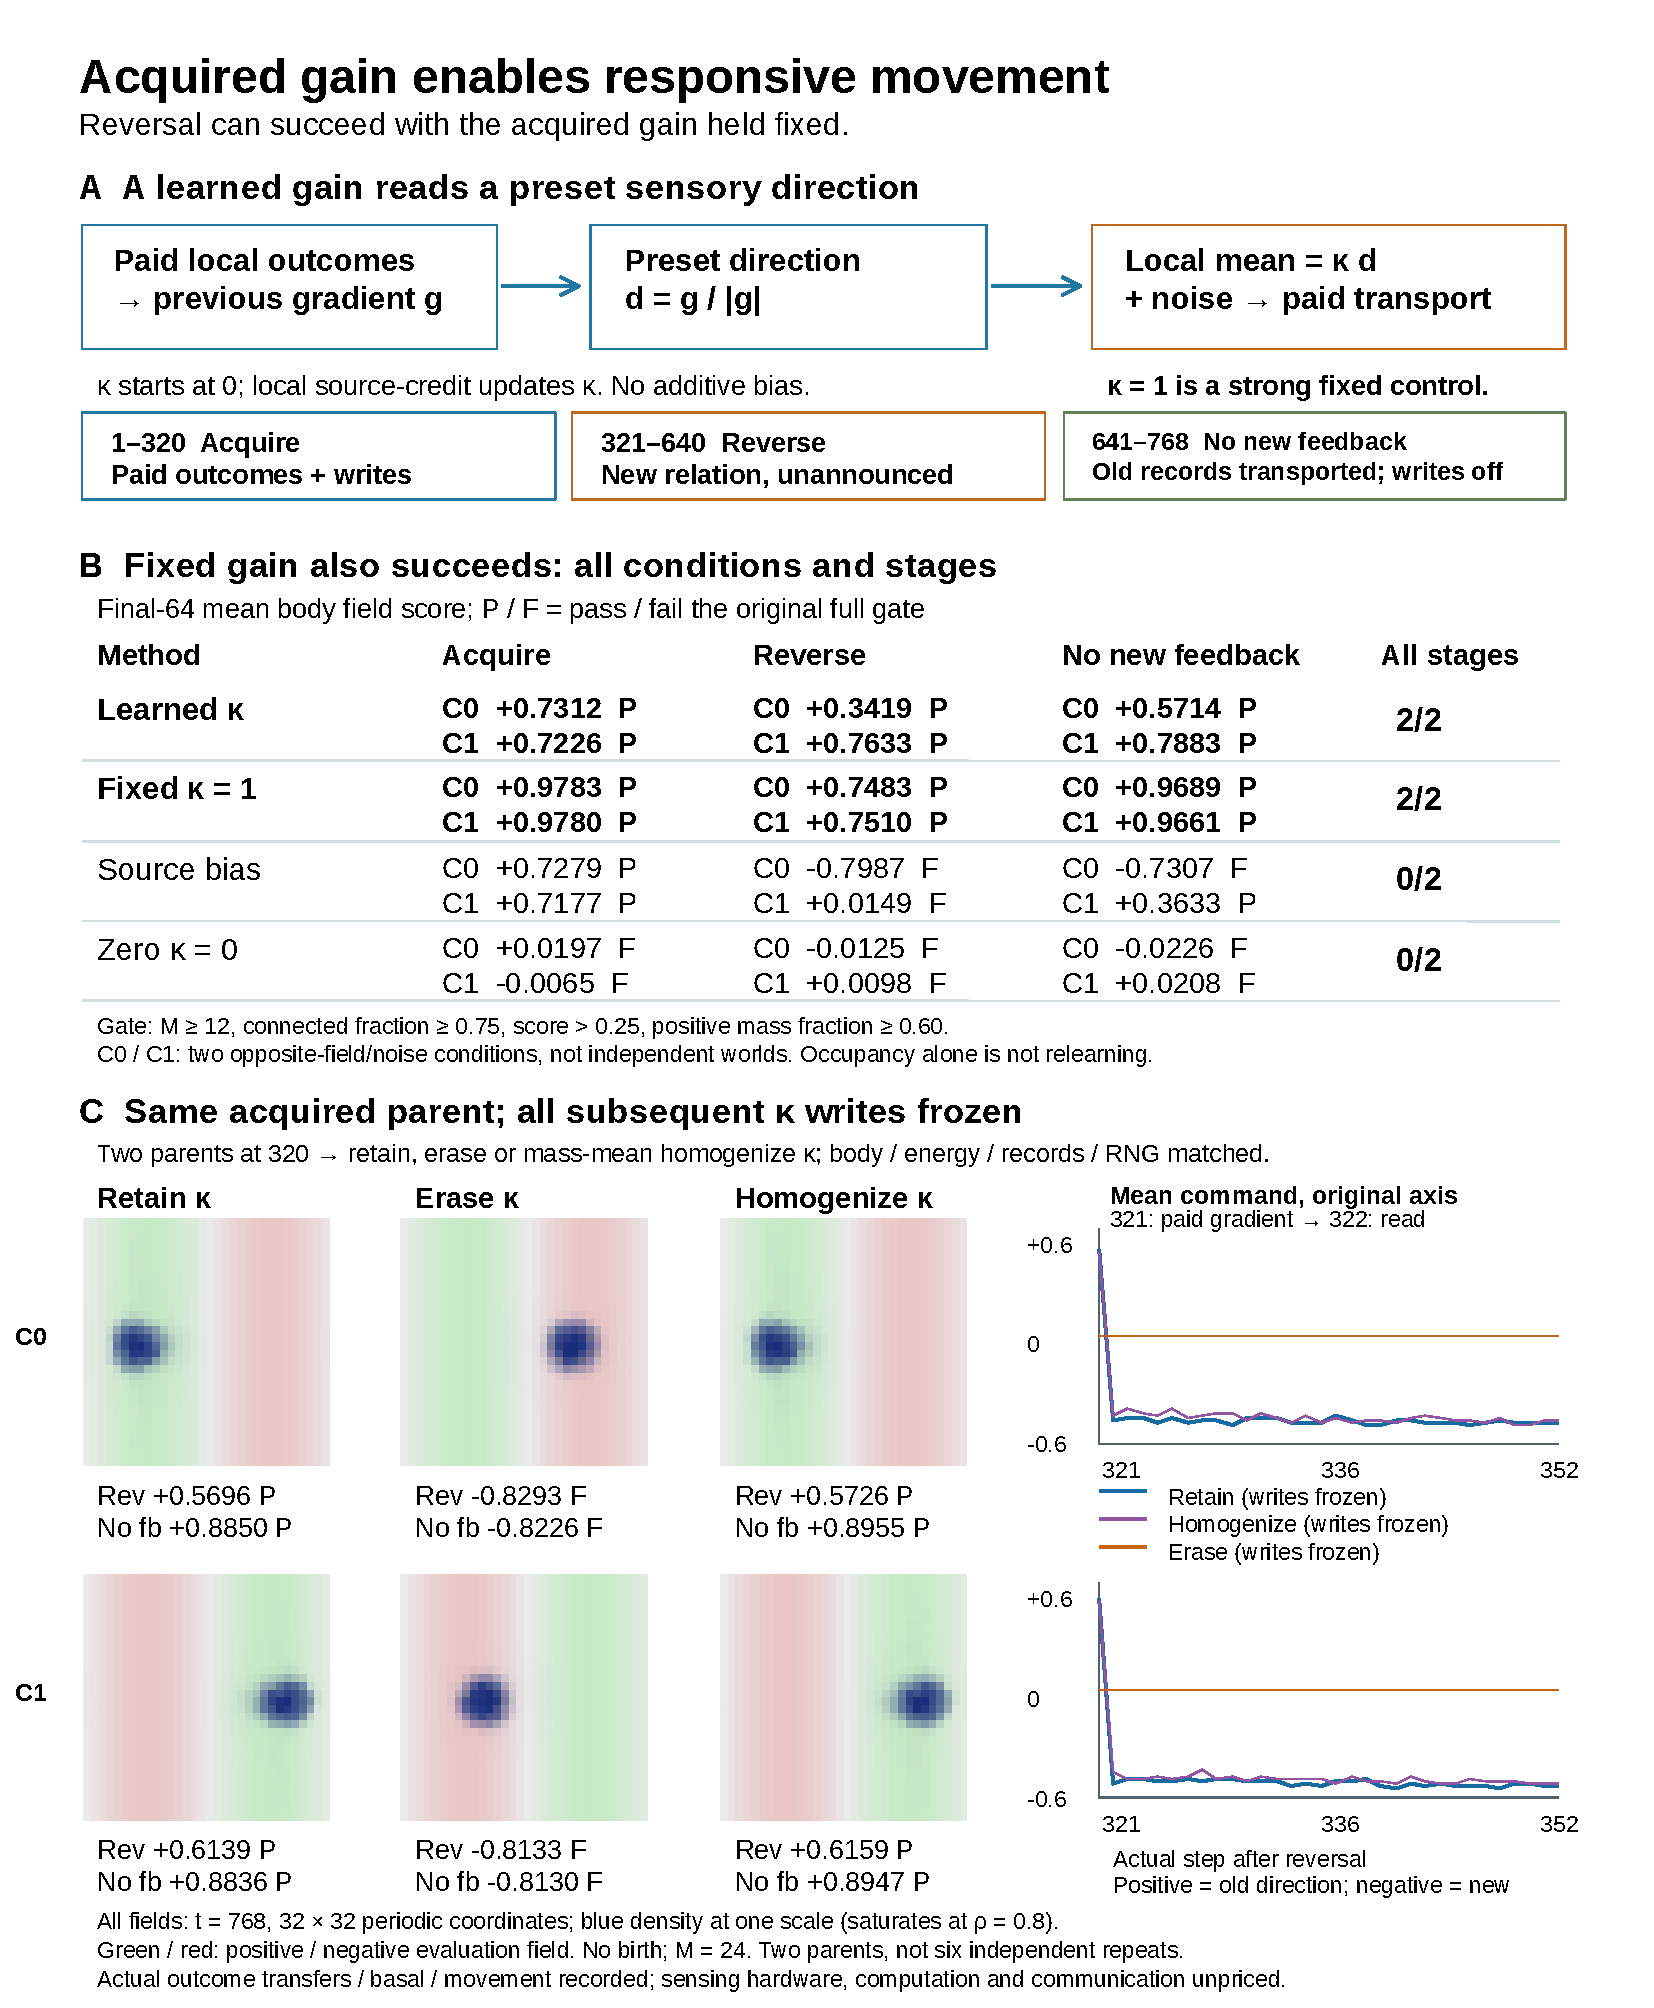
\includegraphics[width=\linewidth,height=0.69\textheight,keepaspectratio]{work/longform_v047/figures/acquired_gain_v0476/acquired_gain.pdf}
\captionsetup{font=footnotesize}
\caption{\textbf{Acquired response gain supports turning without a requirement to relearn the reversal.}
\textbf{a}, A standard local score rule learns an initially zero scalar gain multiplying the direction of a previous actually paid local gradient. Sensory direction and the actuator are supplied. Acquisition and unannounced reversal each last 320 updates; the final 128 add no new payments, observations or writes, while older legal records are transported and read.
\textbf{b}, All four methods and both seed--field conditions retain their final-64 field scores and original composite gates. Learned and fixed positive gain each pass all three phases in both conditions; bias and zero-gain controls do not. Passing the occupancy criterion is not by itself evidence of relearning. Physical costs are reported separately.
\textbf{c}, Two actual acquired parents at 320 supply retained, erased and mass-mean-homogenized gain continuations with gain writing frozen. Retention and homogenization pass both later phases; erasure fails. Curves show the actual mean commands at updates 321--352, not displacement; they change after the new paid observation despite frozen gain. The displayed fields are actual states at update 768 and use original periodic coordinates and a common density scale: blue opacity is $\min(\rho/0.8,1)$, with green/red indicating favourable/unfavourable evaluation fields. Scores under fields describe phase windows, not the displayed snapshot. The six futures are paired interventions from two parents. Homogenization preserves the scalar mean, not each nonlinear action, and global averaging is used only to construct the intervention. All paths remain mass 24 with no tissue birth. Local outcome transfers, basal and movement costs are recorded; computation, communication and sensing hardware have no separate tariff. These results establish a usable acquired response strength, not superiority to fixed positive gain, spatial-pattern necessity, or learning through regeneration.}
\label{fig:acquired-gain}
\end{figure}


\subsection*{Earlier protection-carriage process retained in full}
The original protection figure concerns a separate generative implementation. It is retained alongside, and does not supply an unmeasured life stage of, the predictive-maintenance experiment.
\begin{figure}[p]
\centering
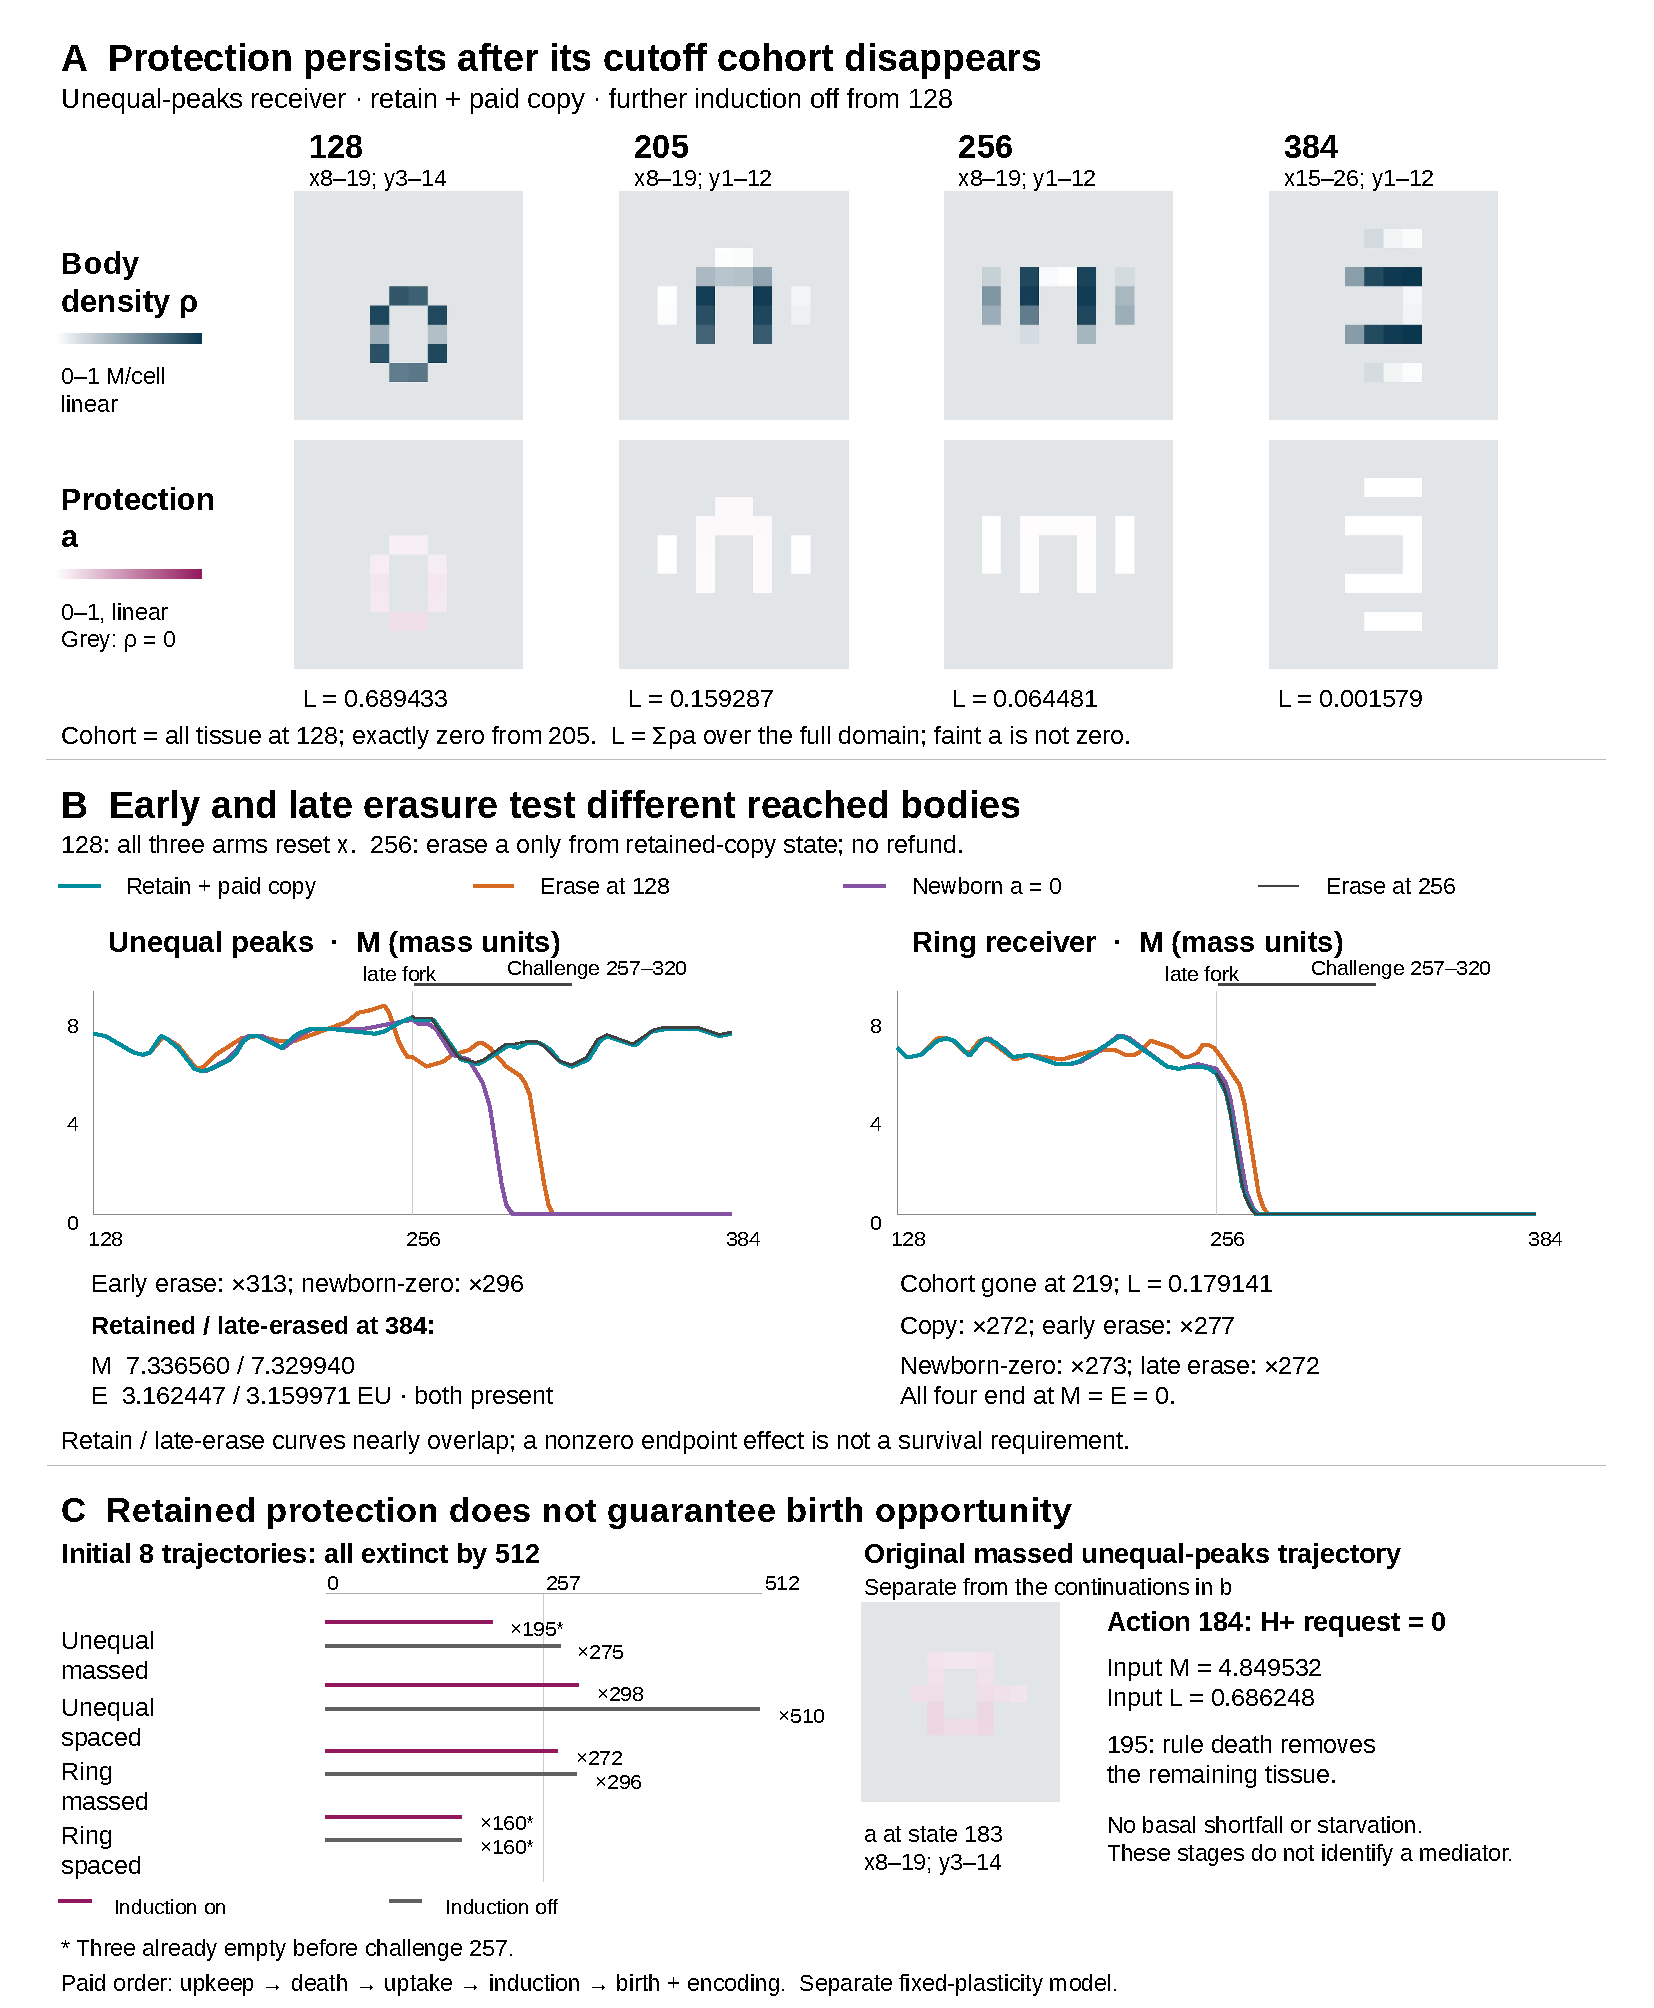
\includegraphics[width=0.95\linewidth]{figures/main/protection/paid_protection_renewal.pdf}
\caption{\textbf{Transmission across tissue replacement and the necessity of residual protection are different questions.}
\textbf{a,} Archived unequal-peaks fields under retained paid copying. All tissue present at cutoff 128 disappears by 205, while load $L=\sum\rho a$ remains nonzero. Each column shows density and protection in one labelled original-coordinate window; both use fixed linear 0--1 scales, with empty cells grey. Further induction is off.
\textbf{b,} Six early continuations and two late-erasure futures, including extinct tails. Early branches share each physical receiver and reset the fast sensor. Late erasure clears only protection at retained-copy state 256, without a refund; retained references are reused. Unequal peaks persist to 384 under both late conditions despite a quantitative difference. The ring loses its cutoff cohort but subsequently fails under all four conditions.
\textbf{c,} All eight original trajectories fail; three are empty before challenge. In the original massed unequal-peaks trajectory, positive birth opportunity disappears at 184 despite protection, before rule death empties the body at 195. This is a separate trajectory from b. Copying and erasure change costs and coupled development; these comparisons identify neither an information-only effect nor a mediator or general adaptation.}
\label{fig:paid-protection-renewal}
\end{figure}

\clearpage
\subsection*{Restricted-action and maintenance source coverage}
The full-precision transcription in \path{work/longform_v047/data/evidence_source_rows_v048.json} hashes nine original CSV/JSON inputs. Two additional registers, \path{local_history_source_rows_v048.json} and \path{physical_state_source_rows_v048.json} in the same directory, preserve eight and twenty-two inputs, respectively. The companion \path{integration_v048.json} identifies eight frozen synthesis handoffs: scalar-only action, motion-observing action, affine action maps, selected-action histories, conditional maintenance, strong physiology, material-carried history and physical response coefficients. These are separate protocols, not one concatenated life. Comparisons with additional directional or displacement observations do not enlarge the scalar-only capability. Tables below include failed gates, dependent continuations, actual costs and the original incomplete maintenance path. Their production invokes no simulator or parameter fit.
\subsection*{Scalar-consequence action learning}
The frozen final handoff is \path{scalar_actuator_relearning_20261019/direction_handoff.json}. Four actual batches total 10,880 native updates and 35.827098 worker seconds: ten life-zero paths and ten dependent branches. K is physical transport only; gradient, location and donor displacement are unavailable to the learner. These tables transcribe original outcomes without fitting, replay or filling failed phases.
\begingroup\scriptsize\setlength{\tabcolsep}{3pt}\setlength{\LTpre}{6pt}\setlength{\LTpost}{6pt}
\begin{longtable}{llllllll}
\caption{All life-zero scalar-feedback phases. B/C denotes batch and seed--actuator condition. B1: accumulated, context, fixed run/tumble and random policies; B2: response estimation. A/R/H denote acquisition, reward reversal and no-new-feedback aftereffect. Values are final-64 scores and favourable-half fractions; P/F retains the original complete gate. Conditions share designed fields and are not population replicates.}\label{tab:scalar-phases}\\
\toprule
B/C & Policy & Phase & $S$ & $p_+$ & $M$ & $E$ & Gate \\
\midrule
\endfirsthead
\toprule
B/C & Policy & Phase & $S$ & $p_+$ & $M$ & $E$ & Gate \\
\midrule
\endhead
1/0 & Accum. & A & 0.45880 & 0.93795 & 24.00000 & 141.47464 & P \\
1/0 & Accum. & R & -0.24106 & 0.29753 & 24.00000 & 112.52269 & F \\
1/0 & Accum. & H & 0.21602 & 0.72717 & 24.00000 & 108.42360 & F \\
1/0 & Context & A & 0.45548 & 0.93331 & 24.00000 & 141.42674 & P \\
1/0 & Context & R & -0.52429 & 0.22949 & 24.00000 & 109.25751 & F \\
1/0 & Context & H & -0.42793 & 0.26866 & 24.00000 & 105.24167 & F \\
1/0 & Run/tumble & A & 0.25860 & 0.80085 & 24.00000 & 139.26813 & P \\
1/0 & Run/tumble & R & -0.02739 & 0.44834 & 24.00000 & 123.41600 & F \\
1/0 & Run/tumble & H & 0.07212 & 0.57151 & 24.00000 & 119.38822 & F \\
1/0 & Random & A & 0.06567 & 0.58982 & 24.00000 & 135.68548 & F \\
1/0 & Random & R & -0.05110 & 0.38835 & 24.00000 & 123.26366 & F \\
1/0 & Random & H & -0.08689 & 0.32797 & 24.00000 & 119.28847 & F \\
1/1 & Accum. & A & 0.46246 & 0.91734 & 24.00000 & 140.77320 & P \\
1/1 & Accum. & R & -0.18498 & 0.22542 & 24.00000 & 113.37151 & F \\
1/1 & Accum. & H & 0.17726 & 0.65875 & 24.00000 & 109.27323 & F \\
1/1 & Context & A & 0.45859 & 0.91103 & 24.00000 & 140.71667 & P \\
1/1 & Context & R & -0.51626 & 0.10088 & 24.00000 & 107.40498 & F \\
1/1 & Context & H & -0.26544 & 0.22956 & 24.00000 & 103.35246 & F \\
1/1 & Run/tumble & A & 0.16078 & 0.65202 & 24.00000 & 136.68917 & F \\
1/1 & Run/tumble & R & -0.01925 & 0.44539 & 24.00000 & 123.34240 & F \\
1/1 & Run/tumble & H & 0.04742 & 0.52039 & 24.00000 & 119.29422 & F \\
1/1 & Random & A & -0.00848 & 0.45700 & 24.00000 & 133.50245 & F \\
1/1 & Random & R & 0.02761 & 0.52943 & 24.00000 & 124.42239 & F \\
1/1 & Random & H & 0.03695 & 0.54288 & 24.00000 & 120.44199 & F \\
2/0 & Response & A & 0.63550 & 0.96765 & 24.00000 & 146.48055 & P \\
2/0 & Response & R & 0.14684 & 0.61446 & 24.00000 & 125.44861 & F \\
2/0 & Response & H & 0.53410 & 0.91177 & 24.00000 & 121.30789 & P \\
2/1 & Response & A & 0.63274 & 0.96494 & 24.00000 & 145.69751 & P \\
2/1 & Response & R & 0.27984 & 0.78357 & 24.00000 & 128.45767 & P \\
2/1 & Response & H & 0.60963 & 0.95065 & 24.00000 & 124.31863 & P \\
\bottomrule
\end{longtable}
\begin{longtable}{llllllll}
\caption{Actual costs for all 46 scalar-feedback phase windows, including dependent continuations. B3 changes acquired content; B4 changes only the actuator. X denotes that actuator-change interval, not reward reversal. Gain and loss are completed outcome transfers; no separate sensor tariff is charged.}\label{tab:scalar-costs}\\
\toprule
B/C & Policy & Phase & Steps & Gain & Loss & Motor & Basal \\
\midrule
\endfirsthead
\toprule
B/C & Policy & Phase & Steps & Gain & Loss & Motor & Basal \\
\midrule
\endhead
1/0 & Accum. & A & 320 & 9.64906 & 2.17522 & 0.78320 & 9.21600 \\
1/0 & Accum. & R & 320 & 1.72337 & 20.40287 & 1.05645 & 9.21600 \\
1/0 & Accum. & H & 128 & 0.00000 & 0.00000 & 0.41269 & 3.68640 \\
1/0 & Context & A & 320 & 9.61796 & 2.19036 & 0.78486 & 9.21600 \\
1/0 & Context & R & 320 & 1.31484 & 23.40674 & 0.86133 & 9.21600 \\
1/0 & Context & H & 128 & 0.00000 & 0.00000 & 0.32943 & 3.68640 \\
1/0 & Run/tumble & A & 320 & 8.06814 & 2.70261 & 0.88141 & 9.21600 \\
1/0 & Run/tumble & R & 320 & 3.14939 & 8.89969 & 0.88583 & 9.21600 \\
1/0 & Run/tumble & H & 128 & 0.00000 & 0.00000 & 0.34138 & 3.68640 \\
1/0 & Random & A & 320 & 5.15571 & 3.53303 & 0.72120 & 9.21600 \\
1/0 & Random & R & 320 & 2.82530 & 5.29983 & 0.73130 & 9.21600 \\
1/0 & Random & H & 128 & 0.00000 & 0.00000 & 0.28879 & 3.68640 \\
1/1 & Accum. & A & 320 & 9.36770 & 2.57411 & 0.80439 & 9.21600 \\
1/1 & Accum. & R & 320 & 1.41087 & 18.59952 & 0.99704 & 9.21600 \\
1/1 & Accum. & H & 128 & 0.00000 & 0.00000 & 0.41188 & 3.68640 \\
1/1 & Context & A & 320 & 9.33387 & 2.59579 & 0.80541 & 9.21600 \\
1/1 & Context & R & 320 & 1.03790 & 24.25615 & 0.87744 & 9.21600 \\
1/1 & Context & H & 128 & 0.00000 & 0.00000 & 0.36612 & 3.68640 \\
1/1 & Run/tumble & A & 320 & 6.70004 & 3.90077 & 0.89410 & 9.21600 \\
1/1 & Run/tumble & R & 320 & 4.76012 & 7.98483 & 0.90606 & 9.21600 \\
1/1 & Run/tumble & H & 128 & 0.00000 & 0.00000 & 0.36178 & 3.68640 \\
1/1 & Random & A & 320 & 4.15902 & 4.71184 & 0.72872 & 9.21600 \\
1/1 & Random & R & 320 & 4.61328 & 3.74541 & 0.73194 & 9.21600 \\
1/1 & Random & H & 128 & 0.00000 & 0.00000 & 0.29400 & 3.68640 \\
2/0 & Response & A & 320 & 14.13818 & 1.42393 & 1.01770 & 9.21600 \\
2/0 & Response & R & 320 & 3.59591 & 14.31667 & 1.09518 & 9.21600 \\
2/0 & Response & H & 128 & 0.00000 & 0.00000 & 0.45432 & 3.68640 \\
2/1 & Response & A & 320 & 13.73607 & 1.79897 & 1.02359 & 9.21600 \\
2/1 & Response & R & 320 & 4.64699 & 11.57446 & 1.09636 & 9.21600 \\
2/1 & Response & H & 128 & 0.00000 & 0.00000 & 0.45264 & 3.68640 \\
3/0 & Clear & H & 128 & 0.00000 & 0.00000 & 0.30716 & 3.68640 \\
3/0 & Rotate & H & 128 & 0.00000 & 0.00000 & 0.45566 & 3.68640 \\
3/1 & Clear & H & 128 & 0.00000 & 0.00000 & 0.30467 & 3.68640 \\
3/1 & Rotate & H & 128 & 0.00000 & 0.00000 & 0.45287 & 3.68640 \\
4/0 & Continue & X & 320 & 29.72727 & 0.08580 & 0.99902 & 9.21600 \\
4/0 & Continue & H & 128 & 0.00000 & 0.00000 & 0.42308 & 3.68640 \\
4/0 & Frozen & X & 320 & 10.75098 & 4.85627 & 1.05909 & 9.21600 \\
4/0 & Frozen & H & 128 & 0.00000 & 0.00000 & 0.42824 & 3.68640 \\
4/0 & Run/tumble & X & 320 & 26.62353 & 0.24493 & 0.87433 & 9.21600 \\
4/0 & Run/tumble & H & 128 & 0.00000 & 0.00000 & 0.32933 & 3.68640 \\
4/1 & Continue & X & 320 & 29.40942 & 0.12737 & 0.97053 & 9.21600 \\
4/1 & Continue & H & 128 & 0.00000 & 0.00000 & 0.41235 & 3.68640 \\
4/1 & Frozen & X & 320 & 10.54381 & 5.96074 & 1.05363 & 9.21600 \\
4/1 & Frozen & H & 128 & 0.00000 & 0.00000 & 0.43361 & 3.68640 \\
4/1 & Run/tumble & X & 320 & 26.67450 & 0.30702 & 0.87516 & 9.21600 \\
4/1 & Run/tumble & H & 128 & 0.00000 & 0.00000 & 0.33494 & 3.68640 \\
\bottomrule
\end{longtable}
\begin{longtable}{llllllll}
\caption{Phase-end physical accounts. Body-time is the integral of living mass over actual updates; zero unpaid/death entries are recorded values. Mass and energy are stocks, not sums.}\label{tab:scalar-physical}\\
\toprule
B/C & Policy & Phase & $M$ & $E$ & Unpaid & Deleted & Body-time \\
\midrule
\endfirsthead
\toprule
B/C & Policy & Phase & $M$ & $E$ & Unpaid & Deleted & Body-time \\
\midrule
\endhead
1/0 & Accum. & A & 24.00000 & 141.47464 & 0.00000 & 0.00000 & 7680.00000 \\
1/0 & Accum. & R & 24.00000 & 112.52269 & 0.00000 & 0.00000 & 7680.00000 \\
1/0 & Accum. & H & 24.00000 & 108.42360 & 0.00000 & 0.00000 & 3072.00000 \\
1/0 & Context & A & 24.00000 & 141.42674 & 0.00000 & 0.00000 & 7680.00000 \\
1/0 & Context & R & 24.00000 & 109.25751 & 0.00000 & 0.00000 & 7680.00000 \\
1/0 & Context & H & 24.00000 & 105.24167 & 0.00000 & 0.00000 & 3072.00000 \\
1/0 & Run/tumble & A & 24.00000 & 139.26813 & 0.00000 & 0.00000 & 7680.00000 \\
1/0 & Run/tumble & R & 24.00000 & 123.41600 & 0.00000 & 0.00000 & 7680.00000 \\
1/0 & Run/tumble & H & 24.00000 & 119.38822 & 0.00000 & 0.00000 & 3072.00000 \\
1/0 & Random & A & 24.00000 & 135.68548 & 0.00000 & 0.00000 & 7680.00000 \\
1/0 & Random & R & 24.00000 & 123.26366 & 0.00000 & 0.00000 & 7680.00000 \\
1/0 & Random & H & 24.00000 & 119.28847 & 0.00000 & 0.00000 & 3072.00000 \\
1/1 & Accum. & A & 24.00000 & 140.77320 & 0.00000 & 0.00000 & 7680.00000 \\
1/1 & Accum. & R & 24.00000 & 113.37151 & 0.00000 & 0.00000 & 7680.00000 \\
1/1 & Accum. & H & 24.00000 & 109.27323 & 0.00000 & 0.00000 & 3072.00000 \\
1/1 & Context & A & 24.00000 & 140.71667 & 0.00000 & 0.00000 & 7680.00000 \\
1/1 & Context & R & 24.00000 & 107.40498 & 0.00000 & 0.00000 & 7680.00000 \\
1/1 & Context & H & 24.00000 & 103.35246 & 0.00000 & 0.00000 & 3072.00000 \\
1/1 & Run/tumble & A & 24.00000 & 136.68917 & 0.00000 & 0.00000 & 7680.00000 \\
1/1 & Run/tumble & R & 24.00000 & 123.34240 & 0.00000 & 0.00000 & 7680.00000 \\
1/1 & Run/tumble & H & 24.00000 & 119.29422 & 0.00000 & 0.00000 & 3072.00000 \\
1/1 & Random & A & 24.00000 & 133.50245 & 0.00000 & 0.00000 & 7680.00000 \\
1/1 & Random & R & 24.00000 & 124.42239 & 0.00000 & 0.00000 & 7680.00000 \\
1/1 & Random & H & 24.00000 & 120.44199 & 0.00000 & 0.00000 & 3072.00000 \\
2/0 & Response & A & 24.00000 & 146.48055 & 0.00000 & 0.00000 & 7680.00000 \\
2/0 & Response & R & 24.00000 & 125.44861 & 0.00000 & 0.00000 & 7680.00000 \\
2/0 & Response & H & 24.00000 & 121.30789 & 0.00000 & 0.00000 & 3072.00000 \\
2/1 & Response & A & 24.00000 & 145.69751 & 0.00000 & 0.00000 & 7680.00000 \\
2/1 & Response & R & 24.00000 & 128.45767 & 0.00000 & 0.00000 & 7680.00000 \\
2/1 & Response & H & 24.00000 & 124.31863 & 0.00000 & 0.00000 & 3072.00000 \\
3/0 & Clear & H & 24.00000 & 121.45505 & 0.00000 & 0.00000 & 3072.00000 \\
3/0 & Rotate & H & 24.00000 & 121.30655 & 0.00000 & 0.00000 & 3072.00000 \\
3/1 & Clear & H & 24.00000 & 124.46660 & 0.00000 & 0.00000 & 3072.00000 \\
3/1 & Rotate & H & 24.00000 & 124.31840 & 0.00000 & 0.00000 & 3072.00000 \\
4/0 & Continue & X & 24.00000 & 165.90701 & 0.00000 & 0.00000 & 7680.00000 \\
4/0 & Continue & H & 24.00000 & 161.79753 & 0.00000 & 0.00000 & 3072.00000 \\
4/0 & Frozen & X & 24.00000 & 142.10017 & 0.00000 & 0.00000 & 7680.00000 \\
4/0 & Frozen & H & 24.00000 & 137.98553 & 0.00000 & 0.00000 & 3072.00000 \\
4/0 & Run/tumble & X & 24.00000 & 162.76882 & 0.00000 & 0.00000 & 7680.00000 \\
4/0 & Run/tumble & H & 24.00000 & 158.75309 & 0.00000 & 0.00000 & 3072.00000 \\
4/1 & Continue & X & 24.00000 & 164.79303 & 0.00000 & 0.00000 & 7680.00000 \\
4/1 & Continue & H & 24.00000 & 160.69428 & 0.00000 & 0.00000 & 3072.00000 \\
4/1 & Frozen & X & 24.00000 & 140.01095 & 0.00000 & 0.00000 & 7680.00000 \\
4/1 & Frozen & H & 24.00000 & 135.89095 & 0.00000 & 0.00000 & 3072.00000 \\
4/1 & Run/tumble & X & 24.00000 & 161.97383 & 0.00000 & 0.00000 & 7680.00000 \\
4/1 & Run/tumble & H & 24.00000 & 157.95249 & 0.00000 & 0.00000 & 3072.00000 \\
\bottomrule
\end{longtable}
\begin{longtable}{lllllll}
\caption{Actual 640-step parents and their no-feedback content interventions. Retained tails are recorded references from B2, not additional executions. Clearing and rotation are four new dependent branches; norm preservation is not command or expense matching.}\label{tab:scalar-content}\\
\toprule
Parent & Content & $S$ & $p_+$ & $E$ & Motor & Gate \\
\midrule
\endfirsthead
\toprule
Parent & Content & $S$ & $p_+$ & $E$ & Motor & Gate \\
\midrule
\endhead
0 & Retained (recorded) & 0.53410 & 0.91177 & 121.30789 & 0.45432 & P \\
0 & Clear & 0.22435 & 0.69697 & 121.45505 & 0.30716 & F \\
0 & Rotate & 0.14044 & 0.61550 & 121.30655 & 0.45566 & F \\
1 & Retained (recorded) & 0.60963 & 0.95065 & 124.31863 & 0.45264 & P \\
1 & Clear & 0.34531 & 0.80976 & 124.46660 & 0.30467 & P \\
1 & Rotate & 0.19537 & 0.62192 & 124.31840 & 0.45287 & F \\
\bottomrule
\end{longtable}
\begin{longtable}{llllllll}
\caption{Actuator-only change from two actual 320-step parents. X lasts 320 paid steps and H lasts 128 steps without new outcomes or writes. The fixed run/tumble control is endowed with the same initial acquired direction. Six continuations are paired branches.}\label{tab:scalar-actuator}\\
\toprule
B/C & Policy & Phase & $S$ & $p_+$ & $M$ & $E$ & Gate \\
\midrule
\endfirsthead
\toprule
B/C & Policy & Phase & $S$ & $p_+$ & $M$ & $E$ & Gate \\
\midrule
\endhead
4/0 & Continue & X & 0.88986 & 0.99463 & 24.00000 & 165.90701 & P \\
4/0 & Continue & H & 0.85625 & 0.99860 & 24.00000 & 161.79753 & P \\
4/0 & Frozen & X & -0.23287 & 0.30229 & 24.00000 & 142.10017 & F \\
4/0 & Frozen & H & -0.25315 & 0.34688 & 24.00000 & 137.98553 & F \\
4/0 & Run/tumble & X & 0.71258 & 0.95895 & 24.00000 & 162.76882 & P \\
4/0 & Run/tumble & H & 0.71991 & 0.95358 & 24.00000 & 158.75309 & P \\
4/1 & Continue & X & 0.86846 & 0.99443 & 24.00000 & 164.79303 & P \\
4/1 & Continue & H & 0.76574 & 0.99779 & 24.00000 & 160.69428 & P \\
4/1 & Frozen & X & -0.29387 & 0.30623 & 24.00000 & 140.01095 & F \\
4/1 & Frozen & H & -0.28662 & 0.30342 & 24.00000 & 135.89095 & F \\
4/1 & Run/tumble & X & 0.70764 & 0.95810 & 24.00000 & 161.97383 & P \\
4/1 & Run/tumble & H & 0.72083 & 0.95011 & 24.00000 & 157.95249 & P \\
\bottomrule
\end{longtable}
\endgroup

\subsection*{Action learning with additional motion and gradient information}
Batch key: K1, original action-map learning; K2, reward versus execution changes separated by the policy name; K3, acquired action-map content; K4, material versus lattice storage; A1, affine learning under reward reversal; A2, affine execution-only change. Policy codes: p1: actuator frozen; p2: actuator write; p3: carried; p4: erase frozen; p5: euler; p6: frozen; p7: iv; p8: nlms; p9: nlms frozen; p10: nlms write; p11: reflex; p12: reward clear; p13: reward frozen; p14: reward homogeneous; p15: reward rotated; p16: reward write. The four transport batches total 16,831 actual updates; the affine sequence totals 7,936. Source-specific observations, methods and independent versus parent-continuation status remain distinct.
\begingroup\scriptsize\setlength{\tabcolsep}{3pt}\setlength{\LTpre}{6pt}\setlength{\LTpost}{6pt}
\begin{longtable}{llllllll}
\caption{All 102 phase windows under richer information interfaces. K batches expose donor displacement and/or a legally recorded gradient; A batches compare affine action-map estimation. A/C/H denote acquisition, the source-defined changed relation and aftereffect. The source register retains which relation changed. These windows are not pooled with scalar-only capability.}\label{tab:rich-action-phases}\\
\toprule
B/C & Policy & Phase & $S$ & $p_+$ & $M$ & $E$ & Gate \\
\midrule
\endfirsthead
\toprule
B/C & Policy & Phase & $S$ & $p_+$ & $M$ & $E$ & Gate \\
\midrule
\endhead
K1/0 & p3 & A & 0.94933 & 0.99972 & 24.00000 & 159.28075 & P \\
K1/0 & p3 & C & 0.21683 & 0.77010 & 24.00000 & 133.91218 & F \\
K1/0 & p3 & H & 0.69253 & 0.98172 & 24.00000 & 129.76632 & P \\
K1/0 & p5 & A & 0.94850 & 0.99965 & 24.00000 & 159.18918 & P \\
K1/0 & p5 & C & 0.19040 & 0.75158 & 24.00000 & 133.01309 & F \\
K1/0 & p5 & H & 0.67706 & 0.98140 & 24.00000 & 128.86838 & P \\
K1/0 & p11 & A & 0.02400 & 0.55401 & 24.00000 & 134.38716 & F \\
K1/0 & p11 & C & 0.82578 & 0.99177 & 24.00000 & 143.62804 & P \\
K1/0 & p11 & H & 0.87617 & 0.99857 & 24.00000 & 139.50805 & P \\
K1/0 & p6 & C & -0.96059 & 0.00027 & 24.00000 & 111.54835 & F \\
K1/0 & p6 & H & -0.90281 & 0.00021 & 24.00000 & 107.39140 & F \\
K1/0 & p4 & C & -0.93405 & 0.00061 & 24.00000 & 113.15428 & F \\
K1/0 & p4 & H & -0.93191 & 0.00103 & 24.00000 & 109.12761 & F \\
K1/1 & p3 & A & 0.94915 & 0.99970 & 24.00000 & 159.37075 & P \\
K1/1 & p3 & C & 0.20039 & 0.75542 & 24.00000 & 133.77382 & F \\
K1/1 & p3 & H & 0.66627 & 0.98074 & 24.00000 & 129.62989 & P \\
K1/1 & p5 & A & 0.94652 & 0.99963 & 24.00000 & 159.19336 & P \\
K1/1 & p5 & C & 0.19422 & 0.74181 & 24.00000 & 133.21814 & F \\
K1/1 & p5 & H & 0.67858 & 0.97981 & 24.00000 & 129.07349 & P \\
K1/1 & p11 & A & -0.03259 & 0.42145 & 24.00000 & 132.54621 & F \\
K1/1 & p11 & C & 0.87549 & 0.99161 & 24.00000 & 143.38261 & P \\
K1/1 & p11 & H & 0.87035 & 0.99866 & 24.00000 & 139.26645 & P \\
K1/1 & p6 & C & -0.96034 & 0.00024 & 24.00000 & 111.65950 & F \\
K1/1 & p6 & H & -0.89732 & 0.00032 & 24.00000 & 107.50429 & F \\
K1/1 & p4 & C & -0.93144 & 0.00063 & 24.00000 & 113.31630 & F \\
K1/1 & p4 & H & -0.92873 & 0.00104 & 24.00000 & 109.28697 & F \\
K2/0 & p16 & C & 0.38941 & 0.88550 & 24.00000 & 138.69087 & P \\
K2/0 & p16 & H & 0.81429 & 0.99463 & 24.00000 & 134.50368 & P \\
K2/0 & p13 & C & 0.38329 & 0.87859 & 24.00000 & 138.55157 & P \\
K2/0 & p13 & H & 0.81175 & 0.99385 & 24.00000 & 134.36321 & P \\
K2/0 & p12 & C & -0.93065 & 0.00064 & 24.00000 & 113.24371 & F \\
K2/0 & p12 & H & -0.92749 & 0.00114 & 24.00000 & 109.19920 & F \\
K2/0 & p2 & C & 0.96323 & 0.99955 & 24.00000 & 185.12576 & P \\
K2/0 & p2 & H & 0.96215 & 0.99960 & 24.00000 & 180.68298 & P \\
K2/0 & p1 & C & 0.04212 & 0.56127 & 24.00000 & 168.27726 & F \\
K2/0 & p1 & H & -0.35850 & 0.11793 & 24.00000 & 164.14321 & F \\
K2/1 & p16 & C & 0.39047 & 0.88480 & 24.00000 & 138.70146 & P \\
K2/1 & p16 & H & 0.81624 & 0.99466 & 24.00000 & 134.51142 & P \\
K2/1 & p13 & C & 0.38372 & 0.87944 & 24.00000 & 138.56095 & P \\
K2/1 & p13 & H & 0.81271 & 0.99385 & 24.00000 & 134.37287 & P \\
K2/1 & p12 & C & -0.93175 & 0.00065 & 24.00000 & 113.28443 & F \\
K2/1 & p12 & H & -0.92926 & 0.00113 & 24.00000 & 109.24046 & F \\
K2/1 & p2 & C & 0.96314 & 0.99960 & 24.00000 & 185.20316 & P \\
K2/1 & p2 & H & 0.96260 & 0.99965 & 24.00000 & 180.76016 & P \\
K2/1 & p1 & C & 0.05639 & 0.59981 & 24.00000 & 168.74740 & F \\
K2/1 & p1 & H & -0.33598 & 0.13769 & 24.00000 & 164.61377 & F \\
K3/0 & p15 & C & -0.90899 & 0.00108 & 24.00000 & 113.42487 & F \\
K3/0 & p15 & H & -0.73371 & 0.00577 & 24.00000 & 109.27566 & F \\
K3/0 & p14 & C & 0.40399 & 0.89174 & 24.00000 & 138.92671 & P \\
K3/0 & p14 & H & 0.82881 & 0.99518 & 24.00000 & 134.73552 & P \\
K3/1 & p15 & C & -0.90401 & 0.00123 & 24.00000 & 113.57698 & F \\
K3/1 & p15 & H & -0.72583 & 0.00672 & 24.00000 & 109.42477 & F \\
K3/1 & p14 & C & 0.40358 & 0.88979 & 24.00000 & 138.89498 & P \\
K3/1 & p14 & H & 0.83003 & 0.99512 & 24.00000 & 134.70335 & P \\
K4/0 & p3 & A & 0.93448 & 0.99957 & 24.00000 & 158.22866 & P \\
K4/0 & p3 & C & 0.06670 & 0.58987 & 24.00000 & 130.59803 & F \\
K4/0 & p3 & H & 0.55812 & 0.96157 & 24.00000 & 126.51998 & P \\
K4/0 & p5 & A & 0.93433 & 0.99950 & 24.00000 & 158.05782 & P \\
K4/0 & p5 & C & 0.06004 & 0.59160 & 24.00000 & 130.37349 & F \\
K4/0 & p5 & H & 0.53307 & 0.96459 & 24.00000 & 126.29605 & P \\
K4/0 & p11 & A & 0.00749 & 0.53795 & 24.00000 & 134.33014 & F \\
K4/0 & p11 & C & 0.00385 & 0.47367 & 24.00000 & 123.87893 & F \\
K4/0 & p11 & H & 0.02549 & 0.58550 & 24.00000 & 119.81791 & F \\
K4/1 & p3 & A & 0.93273 & 0.99957 & 24.00000 & 158.10195 & P \\
K4/1 & p3 & C & 0.07815 & 0.60340 & 24.00000 & 130.74491 & F \\
K4/1 & p3 & H & 0.56955 & 0.96217 & 24.00000 & 126.66610 & P \\
K4/1 & p5 & A & 0.93221 & 0.99953 & 24.00000 & 157.95787 & P \\
K4/1 & p5 & C & 0.06832 & 0.60329 & 24.00000 & 130.51243 & F \\
K4/1 & p5 & H & 0.53753 & 0.96508 & 24.00000 & 126.43434 & P \\
K4/1 & p11 & A & 0.00037 & 0.46624 & 24.00000 & 133.81011 & F \\
A1/0 & p7 & A & 0.95108 & 0.99971 & 24.00000 & 159.40446 & P \\
A1/0 & p7 & C & 0.19249 & 0.74549 & 24.00000 & 133.45013 & F \\
A1/0 & p7 & H & 0.67026 & 0.97917 & 24.00000 & 129.30727 & P \\
A1/0 & p8 & A & 0.94950 & 0.99968 & 24.00000 & 159.33824 & P \\
A1/0 & p8 & C & 0.22136 & 0.76685 & 24.00000 & 134.21724 & F \\
A1/0 & p8 & H & 0.70243 & 0.98168 & 24.00000 & 130.07317 & P \\
A1/1 & p7 & A & 0.94995 & 0.99969 & 24.00000 & 159.29931 & P \\
A1/1 & p7 & C & 0.19193 & 0.74743 & 24.00000 & 133.40351 & F \\
A1/1 & p7 & H & 0.66561 & 0.97954 & 24.00000 & 129.26075 & P \\
A1/1 & p8 & A & 0.94912 & 0.99969 & 24.00000 & 159.26846 & P \\
A1/1 & p8 & C & 0.23021 & 0.77561 & 24.00000 & 134.49195 & F \\
A1/1 & p8 & H & 0.70555 & 0.98260 & 24.00000 & 130.34755 & P \\
A1/2 & p7 & A & 0.93569 & 0.99960 & 24.00000 & 158.27926 & P \\
A1/2 & p7 & C & 0.07745 & 0.60323 & 24.00000 & 130.88750 & F \\
A1/2 & p7 & H & 0.56958 & 0.96315 & 24.00000 & 126.80718 & P \\
A1/2 & p8 & A & 0.93468 & 0.99959 & 24.00000 & 158.28218 & P \\
A1/2 & p8 & C & 0.07831 & 0.60378 & 24.00000 & 130.95108 & F \\
A1/2 & p8 & H & 0.56951 & 0.96254 & 24.00000 & 126.87058 & P \\
A1/3 & p7 & A & 0.93446 & 0.99958 & 24.00000 & 158.17924 & P \\
A1/3 & p7 & C & 0.07321 & 0.59597 & 24.00000 & 130.75964 & F \\
A1/3 & p7 & H & 0.56321 & 0.96316 & 24.00000 & 126.67930 & P \\
A1/3 & p8 & A & 0.93434 & 0.99959 & 24.00000 & 158.22586 & P \\
A1/3 & p8 & C & 0.07104 & 0.59383 & 24.00000 & 130.78735 & F \\
A1/3 & p8 & H & 0.55808 & 0.96295 & 24.00000 & 126.70686 & P \\
A2/0 & p10 & C & 0.96317 & 0.99960 & 24.00000 & 185.19126 & P \\
A2/0 & p10 & H & 0.96246 & 0.99964 & 24.00000 & 180.74585 & P \\
A2/0 & p9 & C & 0.09399 & 0.64005 & 24.00000 & 169.36338 & F \\
A2/0 & p9 & H & -0.29499 & 0.16208 & 24.00000 & 165.22993 & F \\
A2/1 & p10 & C & 0.96352 & 0.99965 & 24.00000 & 185.09722 & P \\
A2/1 & p10 & H & 0.96328 & 0.99967 & 24.00000 & 180.64496 & P \\
A2/1 & p9 & C & 0.04317 & 0.57673 & 24.00000 & 168.37947 & F \\
A2/1 & p9 & H & -0.36112 & 0.11635 & 24.00000 & 164.24528 & F \\
\bottomrule
\end{longtable}
\begin{longtable}{llllllll}
\caption{Whole-phase actual costs for the richer-information comparisons. Steps count the original actual updates. The richer observations and matrix arithmetic are not physically priced by these expense columns.}\label{tab:rich-action-costs}\\
\toprule
B/C & Policy & Phase & Steps & Gain & Loss & Motor & Basal \\
\midrule
\endfirsthead
\toprule
B/C & Policy & Phase & Steps & Gain & Loss & Motor & Basal \\
\midrule
\endhead
K1/0 & p3 & A & 320 & 26.39743 & 0.50659 & 1.39408 & 9.21600 \\
K1/0 & p3 & C & 320 & 2.70516 & 17.75391 & 1.10382 & 9.21600 \\
K1/0 & p3 & H & 128 & 0.00000 & 0.00000 & 0.45946 & 3.68640 \\
K1/0 & p5 & A & 320 & 26.31055 & 0.51270 & 1.39266 & 9.21600 \\
K1/0 & p5 & C & 320 & 2.41364 & 18.27198 & 1.10175 & 9.21600 \\
K1/0 & p5 & H & 128 & 0.00000 & 0.00000 & 0.45831 & 3.68640 \\
K1/0 & p11 & A & 320 & 4.81041 & 4.00633 & 1.20092 & 9.21600 \\
K1/0 & p11 & C & 320 & 20.57787 & 1.00962 & 1.11137 & 9.21600 \\
K1/0 & p11 & H & 128 & 0.00000 & 0.00000 & 0.43359 & 3.68640 \\
K1/0 & p6 & C & 320 & 0.00012 & 36.84450 & 1.67203 & 9.21600 \\
K1/0 & p6 & H & 128 & 0.00000 & 0.00000 & 0.47055 & 3.68640 \\
K1/0 & p4 & C & 320 & 0.00032 & 36.03655 & 0.87424 & 9.21600 \\
K1/0 & p4 & H & 128 & 0.00000 & 0.00000 & 0.34027 & 3.68640 \\
K1/1 & p3 & A & 320 & 26.48590 & 0.50096 & 1.39819 & 9.21600 \\
K1/1 & p3 & C & 320 & 2.55966 & 17.84380 & 1.09679 & 9.21600 \\
K1/1 & p3 & H & 128 & 0.00000 & 0.00000 & 0.45753 & 3.68640 \\
K1/1 & p5 & A & 320 & 26.33795 & 0.52823 & 1.40036 & 9.21600 \\
K1/1 & p5 & C & 320 & 2.48914 & 18.15218 & 1.09618 & 9.21600 \\
K1/1 & p5 & H & 128 & 0.00000 & 0.00000 & 0.45825 & 3.68640 \\
K1/1 & p11 & A & 320 & 3.90617 & 4.95182 & 1.19214 & 9.21600 \\
K1/1 & p11 & C & 320 & 21.90512 & 0.73634 & 1.11638 & 9.21600 \\
K1/1 & p11 & H & 128 & 0.00000 & 0.00000 & 0.42976 & 3.68640 \\
K1/1 & p6 & C & 320 & 0.00004 & 36.83947 & 1.65582 & 9.21600 \\
K1/1 & p6 & H & 128 & 0.00000 & 0.00000 & 0.46881 & 3.68640 \\
K1/1 & p4 & C & 320 & 0.00045 & 35.96875 & 0.87015 & 9.21600 \\
K1/1 & p4 & H & 128 & 0.00000 & 0.00000 & 0.34292 & 3.68640 \\
K2/0 & p16 & C & 320 & 4.65823 & 14.83187 & 1.20024 & 9.21600 \\
K2/0 & p16 & H & 128 & 0.00000 & 0.00000 & 0.50079 & 3.68640 \\
K2/0 & p13 & C & 320 & 4.58625 & 14.89824 & 1.20118 & 9.21600 \\
K2/0 & p13 & H & 128 & 0.00000 & 0.00000 & 0.50197 & 3.68640 \\
K2/0 & p12 & C & 320 & 0.00039 & 35.91618 & 0.90526 & 9.21600 \\
K2/0 & p12 & H & 128 & 0.00000 & 0.00000 & 0.35811 & 3.68640 \\
K2/0 & p2 & C & 320 & 36.85872 & 0.00018 & 1.79754 & 9.21600 \\
K2/0 & p2 & H & 128 & 0.00000 & 0.00000 & 0.75638 & 3.68640 \\
K2/0 & p1 & C & 320 & 20.30255 & 1.00923 & 1.08081 & 9.21600 \\
K2/0 & p1 & H & 128 & 0.00000 & 0.00000 & 0.44765 & 3.68640 \\
K2/1 & p16 & C & 320 & 4.64428 & 14.89751 & 1.20005 & 9.21600 \\
K2/1 & p16 & H & 128 & 0.00000 & 0.00000 & 0.50364 & 3.68640 \\
K2/1 & p13 & C & 320 & 4.56015 & 14.95324 & 1.20070 & 9.21600 \\
K2/1 & p13 & H & 128 & 0.00000 & 0.00000 & 0.50168 & 3.68640 \\
K2/1 & p12 & C & 320 & 0.00041 & 35.96333 & 0.90740 & 9.21600 \\
K2/1 & p12 & H & 128 & 0.00000 & 0.00000 & 0.35757 & 3.68640 \\
K2/1 & p2 & C & 320 & 36.85080 & 0.00004 & 1.80235 & 9.21600 \\
K2/1 & p2 & H & 128 & 0.00000 & 0.00000 & 0.75659 & 3.68640 \\
K2/1 & p1 & C & 320 & 20.64149 & 0.96756 & 1.08129 & 9.21600 \\
K2/1 & p1 & H & 128 & 0.00000 & 0.00000 & 0.44722 & 3.68640 \\
K3/0 & p15 & C & 320 & 0.00050 & 35.45280 & 1.18758 & 9.21600 \\
K3/0 & p15 & H & 128 & 0.00000 & 0.00000 & 0.46281 & 3.68640 \\
K3/0 & p14 & C & 320 & 4.81839 & 14.75327 & 1.20317 & 9.21600 \\
K3/0 & p14 & H & 128 & 0.00000 & 0.00000 & 0.50478 & 3.68640 \\
K3/1 & p15 & C & 320 & 0.00073 & 35.39149 & 1.18702 & 9.21600 \\
K3/1 & p15 & H & 128 & 0.00000 & 0.00000 & 0.46581 & 3.68640 \\
K3/1 & p14 & C & 320 & 4.78609 & 14.84308 & 1.20278 & 9.21600 \\
K3/1 & p14 & H & 128 & 0.00000 & 0.00000 & 0.50523 & 3.68640 \\
K4/0 & p3 & A & 320 & 25.13390 & 0.52566 & 1.16358 & 9.21600 \\
K4/0 & p3 & C & 320 & 1.47080 & 18.97580 & 0.90964 & 9.21600 \\
K4/0 & p3 & H & 128 & 0.00000 & 0.00000 & 0.39164 & 3.68640 \\
K4/0 & p5 & A & 320 & 24.98344 & 0.53811 & 1.17151 & 9.21600 \\
K4/0 & p5 & C & 320 & 1.39791 & 18.95873 & 0.90750 & 9.21600 \\
K4/0 & p5 & H & 128 & 0.00000 & 0.00000 & 0.39104 & 3.68640 \\
K4/0 & p11 & A & 320 & 4.17110 & 3.65172 & 0.97324 & 9.21600 \\
K4/0 & p11 & C & 320 & 3.53836 & 3.82051 & 0.95306 & 9.21600 \\
K4/0 & p11 & H & 128 & 0.00000 & 0.00000 & 0.37462 & 3.68640 \\
K4/1 & p3 & A & 320 & 25.02951 & 0.54610 & 1.16545 & 9.21600 \\
K4/1 & p3 & C & 320 & 1.53465 & 18.76284 & 0.91285 & 9.21600 \\
K4/1 & p3 & H & 128 & 0.00000 & 0.00000 & 0.39241 & 3.68640 \\
K4/1 & p5 & A & 320 & 24.88910 & 0.54825 & 1.16698 & 9.21600 \\
K4/1 & p5 & C & 320 & 1.43556 & 18.75715 & 0.90785 & 9.21600 \\
K4/1 & p5 & H & 128 & 0.00000 & 0.00000 & 0.39169 & 3.68640 \\
K4/1 & p11 & A & 319 & 10.64716 & 10.59116 & 1.05870 & 9.18720 \\
A1/0 & p7 & A & 320 & 26.50833 & 0.49024 & 1.39763 & 9.21600 \\
A1/0 & p7 & C & 320 & 2.49636 & 18.12968 & 1.10501 & 9.21600 \\
A1/0 & p7 & H & 128 & 0.00000 & 0.00000 & 0.45646 & 3.68640 \\
A1/0 & p8 & A & 320 & 26.44551 & 0.49206 & 1.39921 & 9.21600 \\
A1/0 & p8 & C & 320 & 2.76492 & 17.57241 & 1.09751 & 9.21600 \\
A1/0 & p8 & H & 128 & 0.00000 & 0.00000 & 0.45767 & 3.68640 \\
A1/1 & p7 & A & 320 & 26.40900 & 0.49150 & 1.40219 & 9.21600 \\
A1/1 & p7 & C & 320 & 2.47245 & 18.05344 & 1.09881 & 9.21600 \\
A1/1 & p7 & H & 128 & 0.00000 & 0.00000 & 0.45636 & 3.68640 \\
A1/1 & p8 & A & 320 & 26.37025 & 0.48667 & 1.39912 & 9.21600 \\
A1/1 & p8 & C & 320 & 2.84311 & 17.31390 & 1.08972 & 9.21600 \\
A1/1 & p8 & H & 128 & 0.00000 & 0.00000 & 0.45800 & 3.68640 \\
A1/2 & p7 & A & 320 & 25.18546 & 0.52527 & 1.16494 & 9.21600 \\
A1/2 & p7 & C & 320 & 1.54590 & 18.80860 & 0.91306 & 9.21600 \\
A1/2 & p7 & H & 128 & 0.00000 & 0.00000 & 0.39391 & 3.68640 \\
A1/2 & p8 & A & 320 & 25.18742 & 0.51839 & 1.17085 & 9.21600 \\
A1/2 & p8 & C & 320 & 1.55628 & 18.75829 & 0.91309 & 9.21600 \\
A1/2 & p8 & H & 128 & 0.00000 & 0.00000 & 0.39409 & 3.68640 \\
A1/3 & p7 & A & 320 & 25.07533 & 0.51803 & 1.16207 & 9.21600 \\
A1/3 & p7 & C & 320 & 1.51465 & 18.80602 & 0.91222 & 9.21600 \\
A1/3 & p7 & H & 128 & 0.00000 & 0.00000 & 0.39394 & 3.68640 \\
A1/3 & p8 & A & 320 & 25.12034 & 0.51190 & 1.16659 & 9.21600 \\
A1/3 & p8 & C & 320 & 1.50047 & 18.81162 & 0.91136 & 9.21600 \\
A1/3 & p8 & H & 128 & 0.00000 & 0.00000 & 0.39409 & 3.68640 \\
A2/0 & p10 & C & 320 & 36.88781 & 0.00003 & 1.81876 & 9.21600 \\
A2/0 & p10 & H & 128 & 0.00000 & 0.00000 & 0.75902 & 3.68640 \\
A2/0 & p9 & C & 320 & 21.14770 & 0.82391 & 1.08265 & 9.21600 \\
A2/0 & p9 & H & 128 & 0.00000 & 0.00000 & 0.44705 & 3.68640 \\
A2/1 & p10 & C & 320 & 36.87400 & 0.00000 & 1.82924 & 9.21600 \\
A2/1 & p10 & H & 128 & 0.00000 & 0.00000 & 0.76586 & 3.68640 \\
A2/1 & p9 & C & 320 & 20.44527 & 1.03584 & 1.08242 & 9.21600 \\
A2/1 & p9 & H & 128 & 0.00000 & 0.00000 & 0.44779 & 3.68640 \\
\bottomrule
\end{longtable}
\begin{longtable}{llllllll}
\caption{Recorded physical qualification of the richer-information phases. A dash means the column is absent from that batch summary, not zero or failed survival. The connected fraction in K is a separate condition from survival; fixed-reflex fragmentation must not be called extinction.}\label{tab:rich-action-physical}\\
\toprule
B/C & Policy & Phase & Connected & Unpaid & Deleted & Body-time & Alive \\
\midrule
\endfirsthead
\toprule
B/C & Policy & Phase & Connected & Unpaid & Deleted & Body-time & Alive \\
\midrule
\endhead
K1/0 & p3 & A & 0.99737 & 0.00000 & 0.00000 & 7680.00000 & P \\
K1/0 & p3 & C & 0.99983 & 0.00000 & 0.00000 & 7680.00000 & P \\
K1/0 & p3 & H & 0.99710 & 0.00000 & 0.00000 & 3072.00000 & P \\
K1/0 & p5 & A & 0.99723 & 0.00000 & 0.00000 & 7680.00000 & P \\
K1/0 & p5 & C & 0.99988 & 0.00000 & 0.00000 & 7680.00000 & P \\
K1/0 & p5 & H & 0.99725 & 0.00000 & 0.00000 & 3072.00000 & P \\
K1/0 & p11 & A & 0.99340 & 0.00000 & 0.00000 & 7680.00000 & P \\
K1/0 & p11 & C & 0.99424 & 0.00000 & 0.00000 & 7680.00000 & P \\
K1/0 & p11 & H & 0.99762 & 0.00000 & 0.00000 & 3072.00000 & P \\
K1/0 & p6 & C & 0.99910 & 0.00000 & 0.00000 & 7680.00000 & P \\
K1/0 & p6 & H & 0.99912 & 0.00000 & 0.00000 & 3072.00000 & P \\
K1/0 & p4 & C & 0.99588 & 0.00000 & 0.00000 & 7680.00000 & P \\
K1/0 & p4 & H & 0.99528 & 0.00000 & 0.00000 & 3072.00000 & P \\
K1/1 & p3 & A & 0.99709 & 0.00000 & 0.00000 & 7680.00000 & P \\
K1/1 & p3 & C & 0.99978 & 0.00000 & 0.00000 & 7680.00000 & P \\
K1/1 & p3 & H & 0.99716 & 0.00000 & 0.00000 & 3072.00000 & P \\
K1/1 & p5 & A & 0.99686 & 0.00000 & 0.00000 & 7680.00000 & P \\
K1/1 & p5 & C & 0.99982 & 0.00000 & 0.00000 & 7680.00000 & P \\
K1/1 & p5 & H & 0.99713 & 0.00000 & 0.00000 & 3072.00000 & P \\
K1/1 & p11 & A & 0.99557 & 0.00000 & 0.00000 & 7680.00000 & P \\
K1/1 & p11 & C & 0.99397 & 0.00000 & 0.00000 & 7680.00000 & P \\
K1/1 & p11 & H & 0.99738 & 0.00000 & 0.00000 & 3072.00000 & P \\
K1/1 & p6 & C & 0.99911 & 0.00000 & 0.00000 & 7680.00000 & P \\
K1/1 & p6 & H & 0.99899 & 0.00000 & 0.00000 & 3072.00000 & P \\
K1/1 & p4 & C & 0.99576 & 0.00000 & 0.00000 & 7680.00000 & P \\
K1/1 & p4 & H & 0.99527 & 0.00000 & 0.00000 & 3072.00000 & P \\
K2/0 & p16 & C & 0.99968 & 0.00000 & 0.00000 & 7680.00000 & P \\
K2/0 & p16 & H & 0.99556 & 0.00000 & 0.00000 & 3072.00000 & P \\
K2/0 & p13 & C & 0.99965 & 0.00000 & 0.00000 & 7680.00000 & P \\
K2/0 & p13 & H & 0.99534 & 0.00000 & 0.00000 & 3072.00000 & P \\
K2/0 & p12 & C & 0.99577 & 0.00000 & 0.00000 & 7680.00000 & P \\
K2/0 & p12 & H & 0.99527 & 0.00000 & 0.00000 & 3072.00000 & P \\
K2/0 & p2 & C & 0.99928 & 0.00000 & 0.00000 & 7680.00000 & P \\
K2/0 & p2 & H & 0.99928 & 0.00000 & 0.00000 & 3072.00000 & P \\
K2/0 & p1 & C & 0.99993 & 0.00000 & 0.00000 & 7680.00000 & P \\
K2/0 & p1 & H & 0.99970 & 0.00000 & 0.00000 & 3072.00000 & P \\
K2/1 & p16 & C & 0.99970 & 0.00000 & 0.00000 & 7680.00000 & P \\
K2/1 & p16 & H & 0.99522 & 0.00000 & 0.00000 & 3072.00000 & P \\
K2/1 & p13 & C & 0.99971 & 0.00000 & 0.00000 & 7680.00000 & P \\
K2/1 & p13 & H & 0.99510 & 0.00000 & 0.00000 & 3072.00000 & P \\
K2/1 & p12 & C & 0.99597 & 0.00000 & 0.00000 & 7680.00000 & P \\
K2/1 & p12 & H & 0.99528 & 0.00000 & 0.00000 & 3072.00000 & P \\
K2/1 & p2 & C & 0.99925 & 0.00000 & 0.00000 & 7680.00000 & P \\
K2/1 & p2 & H & 0.99926 & 0.00000 & 0.00000 & 3072.00000 & P \\
K2/1 & p1 & C & 0.99994 & 0.00000 & 0.00000 & 7680.00000 & P \\
K2/1 & p1 & H & 0.99983 & 0.00000 & 0.00000 & 3072.00000 & P \\
K3/0 & p15 & C & 0.99630 & 0.00000 & 0.00000 & 7680.00000 & P \\
K3/0 & p15 & H & 0.99924 & 0.00000 & 0.00000 & 3072.00000 & P \\
K3/0 & p14 & C & 0.99967 & 0.00000 & 0.00000 & 7680.00000 & P \\
K3/0 & p14 & H & 0.99502 & 0.00000 & 0.00000 & 3072.00000 & P \\
K3/1 & p15 & C & 0.99617 & 0.00000 & 0.00000 & 7680.00000 & P \\
K3/1 & p15 & H & 0.99929 & 0.00000 & 0.00000 & 3072.00000 & P \\
K3/1 & p14 & C & 0.99970 & 0.00000 & 0.00000 & 7680.00000 & P \\
K3/1 & p14 & H & 0.99503 & 0.00000 & 0.00000 & 3072.00000 & P \\
K4/0 & p3 & A & 0.99657 & 0.00000 & 0.00000 & 7680.00000 & P \\
K4/0 & p3 & C & 0.99967 & 0.00000 & 0.00000 & 7680.00000 & P \\
K4/0 & p3 & H & 0.99865 & 0.00000 & 0.00000 & 3072.00000 & P \\
K4/0 & p5 & A & 0.99691 & 0.00000 & 0.00000 & 7680.00000 & P \\
K4/0 & p5 & C & 0.99966 & 0.00000 & 0.00000 & 7680.00000 & P \\
K4/0 & p5 & H & 0.99896 & 0.00000 & 0.00000 & 3072.00000 & P \\
K4/0 & p11 & A & 0.99338 & 0.00000 & 0.00000 & 7680.00000 & P \\
K4/0 & p11 & C & 0.97310 & 0.00000 & 0.00000 & 7680.00000 & P \\
K4/0 & p11 & H & 0.99208 & 0.00000 & 0.00000 & 3072.00000 & P \\
K4/1 & p3 & A & 0.99697 & 0.00000 & 0.00000 & 7680.00000 & P \\
K4/1 & p3 & C & 0.99966 & 0.00000 & 0.00000 & 7680.00000 & P \\
K4/1 & p3 & H & 0.99872 & 0.00000 & 0.00000 & 3072.00000 & P \\
K4/1 & p5 & A & 0.99698 & 0.00000 & 0.00000 & 7680.00000 & P \\
K4/1 & p5 & C & 0.99972 & 0.00000 & 0.00000 & 7680.00000 & P \\
K4/1 & p5 & H & 0.99883 & 0.00000 & 0.00000 & 3072.00000 & P \\
K4/1 & p11 & A & 0.66172 & 0.00000 & 0.00000 & 7656.00000 & F \\
A1/0 & p7 & A & -- & 0.00000 & 0.00000 & 7680.00000 & P \\
A1/0 & p7 & C & -- & 0.00000 & 0.00000 & 7680.00000 & P \\
A1/0 & p7 & H & -- & 0.00000 & 0.00000 & 3072.00000 & P \\
A1/0 & p8 & A & -- & 0.00000 & 0.00000 & 7680.00000 & P \\
A1/0 & p8 & C & -- & 0.00000 & 0.00000 & 7680.00000 & P \\
A1/0 & p8 & H & -- & 0.00000 & 0.00000 & 3072.00000 & P \\
A1/1 & p7 & A & -- & 0.00000 & 0.00000 & 7680.00000 & P \\
A1/1 & p7 & C & -- & 0.00000 & 0.00000 & 7680.00000 & P \\
A1/1 & p7 & H & -- & 0.00000 & 0.00000 & 3072.00000 & P \\
A1/1 & p8 & A & -- & 0.00000 & 0.00000 & 7680.00000 & P \\
A1/1 & p8 & C & -- & 0.00000 & 0.00000 & 7680.00000 & P \\
A1/1 & p8 & H & -- & 0.00000 & 0.00000 & 3072.00000 & P \\
A1/2 & p7 & A & -- & 0.00000 & 0.00000 & 7680.00000 & P \\
A1/2 & p7 & C & -- & 0.00000 & 0.00000 & 7680.00000 & P \\
A1/2 & p7 & H & -- & 0.00000 & 0.00000 & 3072.00000 & P \\
A1/2 & p8 & A & -- & 0.00000 & 0.00000 & 7680.00000 & P \\
A1/2 & p8 & C & -- & 0.00000 & 0.00000 & 7680.00000 & P \\
A1/2 & p8 & H & -- & 0.00000 & 0.00000 & 3072.00000 & P \\
A1/3 & p7 & A & -- & 0.00000 & 0.00000 & 7680.00000 & P \\
A1/3 & p7 & C & -- & 0.00000 & 0.00000 & 7680.00000 & P \\
A1/3 & p7 & H & -- & 0.00000 & 0.00000 & 3072.00000 & P \\
A1/3 & p8 & A & -- & 0.00000 & 0.00000 & 7680.00000 & P \\
A1/3 & p8 & C & -- & 0.00000 & 0.00000 & 7680.00000 & P \\
A1/3 & p8 & H & -- & 0.00000 & 0.00000 & 3072.00000 & P \\
A2/0 & p10 & C & -- & 0.00000 & 0.00000 & 7680.00000 & P \\
A2/0 & p10 & H & -- & 0.00000 & 0.00000 & 3072.00000 & P \\
A2/0 & p9 & C & -- & 0.00000 & 0.00000 & 7680.00000 & P \\
A2/0 & p9 & H & -- & 0.00000 & 0.00000 & 3072.00000 & P \\
A2/1 & p10 & C & -- & 0.00000 & 0.00000 & 7680.00000 & P \\
A2/1 & p10 & H & -- & 0.00000 & 0.00000 & 3072.00000 & P \\
A2/1 & p9 & C & -- & 0.00000 & 0.00000 & 7680.00000 & P \\
A2/1 & p9 & H & -- & 0.00000 & 0.00000 & 3072.00000 & P \\
\bottomrule
\end{longtable}
\endgroup

\subsection*{Literal and filtered history controls}
The nine continuous paths comprise 7,128 actual updates; eighteen dependent content interventions add 108. The latter completed their physical work but failed an internal 8 MiB packaging assertion at approximately 10.03 MB, below the project's 128 MiB limit. Their recovered recorded results are used without rerun; the job is not represented as a successful wrapper exit. Total worker time is 10.552385 seconds.
\begingroup\scriptsize\setlength{\tabcolsep}{3pt}\setlength{\LTpre}{6pt}\setlength{\LTpost}{6pt}
\begin{longtable}{lllllll}
\caption{All 36 history-learning stages. Seeds 0--2 are 202610199721--202610199723, shared across the three methods. Each of nine continuous paths supplies four stages.}\label{tab:history-stages}\\
\toprule
Seed & Readout & Stage & Correct & Episodes & $E_{end}$ & Signed move \\
\midrule
\endfirsthead
\toprule
Seed & Readout & Stage & Correct & Episodes & $E_{end}$ & Signed move \\
\midrule
\endhead
0 & Literal & A & 18 & 24 & 65.05668 & 6.20426 \\
0 & Literal & H & 12 & 12 & 62.98564 & 6.07306 \\
0 & Literal & C & 12 & 24 & 53.10955 & 0.22699 \\
0 & Literal & HC & 12 & 12 & 51.04947 & 5.86087 \\
0 & Filtered & A & 21 & 24 & 66.44494 & 9.28288 \\
0 & Filtered & H & 12 & 12 & 64.36717 & 6.01016 \\
0 & Filtered & C & 18 & 24 & 57.34506 & 5.79687 \\
0 & Filtered & HC & 12 & 12 & 55.27877 & 5.78962 \\
0 & Body readout & A & 11 & 24 & 61.60151 & -1.03485 \\
0 & Body readout & H & 5 & 12 & 56.18642 & -0.97866 \\
0 & Body readout & C & 13 & 24 & 46.78967 & 1.00281 \\
0 & Body readout & HC & 8 & 12 & 42.81112 & 1.92796 \\
1 & Literal & A & 18 & 24 & 65.04942 & 6.23742 \\
1 & Literal & H & 12 & 12 & 62.97188 & 6.10287 \\
1 & Literal & C & 12 & 24 & 53.06316 & 0.06955 \\
1 & Literal & HC & 12 & 12 & 50.99178 & 5.97483 \\
1 & Filtered & A & 21 & 24 & 66.44040 & 9.28821 \\
1 & Filtered & H & 12 & 12 & 64.35977 & 5.99645 \\
1 & Filtered & C & 18 & 24 & 57.32632 & 5.95765 \\
1 & Filtered & HC & 12 & 12 & 55.25413 & 5.87864 \\
1 & Body readout & A & 12 & 24 & 62.08055 & 0.12961 \\
1 & Body readout & H & 5 & 12 & 56.65039 & -1.00043 \\
1 & Body readout & C & 9 & 24 & 45.30551 & -2.88229 \\
1 & Body readout & HC & 6 & 12 & 40.35288 & -0.00024 \\
2 & Literal & A & 18 & 24 & 65.05367 & 6.34841 \\
2 & Literal & H & 12 & 12 & 62.97794 & 6.00466 \\
2 & Literal & C & 12 & 24 & 53.07760 & -0.42245 \\
2 & Literal & HC & 12 & 12 & 51.01084 & 5.83897 \\
2 & Filtered & A & 21 & 24 & 66.43916 & 9.40026 \\
2 & Filtered & H & 12 & 12 & 64.35711 & 5.95416 \\
2 & Filtered & C & 18 & 24 & 57.32790 & 5.76016 \\
2 & Filtered & HC & 12 & 12 & 55.25642 & 5.87650 \\
2 & Body readout & A & 12 & 24 & 62.07464 & 0.02093 \\
2 & Body readout & H & 9 & 12 & 58.55977 & 2.98598 \\
2 & Body readout & C & 12 & 24 & 48.65910 & -0.01282 \\
2 & Body readout & HC & 3 & 12 & 42.26660 & -2.89651 \\
\bottomrule
\end{longtable}
\begin{longtable}{lllllllll}
\caption{Actual expenses in all history-learning stages. Sensor and feedback fees here are explicit task tariffs, unlike the scalar action model. These comparisons do not assign a full physical cost to central table lookup or table capacity.}\label{tab:history-costs}\\
\toprule
Seed & Readout & Stage & Motor & Basal & Sensor & Outcome fee & Gain & Loss \\
\midrule
\endfirsthead
\toprule
Seed & Readout & Stage & Motor & Basal & Sensor & Outcome fee & Gain & Loss \\
\midrule
\endhead
0 & Literal & A & 0.95292 & 7.60320 & 0.69120 & 0.57600 & 4.32000 & 1.44000 \\
0 & Literal & H & 0.51584 & 3.80160 & 0.34560 & 0.28800 & 2.88000 & 0.00000 \\
0 & Literal & C & 1.00569 & 7.60320 & 0.69120 & 0.57600 & 2.88000 & 2.88000 \\
0 & Literal & HC & 0.50488 & 3.80160 & 0.34560 & 0.28800 & 2.88000 & 0.00000 \\
0 & Filtered & A & 1.00466 & 7.60320 & 0.69120 & 0.57600 & 5.04000 & 0.72000 \\
0 & Filtered & H & 0.52258 & 3.80160 & 0.34560 & 0.28800 & 2.88000 & 0.00000 \\
0 & Filtered & C & 1.03170 & 7.60320 & 0.69120 & 0.57600 & 4.32000 & 1.44000 \\
0 & Filtered & HC & 0.51110 & 3.80160 & 0.34560 & 0.28800 & 2.88000 & 0.00000 \\
0 & Body readout & A & 1.04809 & 7.60320 & 0.69120 & 0.57600 & 2.64000 & 3.12000 \\
0 & Body readout & H & 0.49989 & 3.80160 & 0.34560 & 0.28800 & 1.20000 & 1.68000 \\
0 & Body readout & C & 1.00635 & 7.60320 & 0.69120 & 0.57600 & 3.12000 & 2.64000 \\
0 & Body readout & HC & 0.50335 & 3.80160 & 0.34560 & 0.28800 & 1.92000 & 0.96000 \\
1 & Literal & A & 0.96018 & 7.60320 & 0.69120 & 0.57600 & 4.32000 & 1.44000 \\
1 & Literal & H & 0.52234 & 3.80160 & 0.34560 & 0.28800 & 2.88000 & 0.00000 \\
1 & Literal & C & 1.03832 & 7.60320 & 0.69120 & 0.57600 & 2.88000 & 2.88000 \\
1 & Literal & HC & 0.51618 & 3.80160 & 0.34560 & 0.28800 & 2.88000 & 0.00000 \\
1 & Filtered & A & 1.00920 & 7.60320 & 0.69120 & 0.57600 & 5.04000 & 0.72000 \\
1 & Filtered & H & 0.52543 & 3.80160 & 0.34560 & 0.28800 & 2.88000 & 0.00000 \\
1 & Filtered & C & 1.04305 & 7.60320 & 0.69120 & 0.57600 & 4.32000 & 1.44000 \\
1 & Filtered & HC & 0.51699 & 3.80160 & 0.34560 & 0.28800 & 2.88000 & 0.00000 \\
1 & Body readout & A & 1.04905 & 7.60320 & 0.69120 & 0.57600 & 2.88000 & 2.88000 \\
1 & Body readout & H & 0.51496 & 3.80160 & 0.34560 & 0.28800 & 1.20000 & 1.68000 \\
1 & Body readout & C & 1.03448 & 7.60320 & 0.69120 & 0.57600 & 2.16000 & 3.60000 \\
1 & Body readout & HC & 0.51743 & 3.80160 & 0.34560 & 0.28800 & 1.44000 & 1.44000 \\
2 & Literal & A & 0.95593 & 7.60320 & 0.69120 & 0.57600 & 4.32000 & 1.44000 \\
2 & Literal & H & 0.52053 & 3.80160 & 0.34560 & 0.28800 & 2.88000 & 0.00000 \\
2 & Literal & C & 1.02994 & 7.60320 & 0.69120 & 0.57600 & 2.88000 & 2.88000 \\
2 & Literal & HC & 0.51156 & 3.80160 & 0.34560 & 0.28800 & 2.88000 & 0.00000 \\
2 & Filtered & A & 1.01044 & 7.60320 & 0.69120 & 0.57600 & 5.04000 & 0.72000 \\
2 & Filtered & H & 0.52685 & 3.80160 & 0.34560 & 0.28800 & 2.88000 & 0.00000 \\
2 & Filtered & C & 1.03880 & 7.60320 & 0.69120 & 0.57600 & 4.32000 & 1.44000 \\
2 & Filtered & HC & 0.51628 & 3.80160 & 0.34560 & 0.28800 & 2.88000 & 0.00000 \\
2 & Body readout & A & 1.05496 & 7.60320 & 0.69120 & 0.57600 & 2.88000 & 2.88000 \\
2 & Body readout & H & 0.51967 & 3.80160 & 0.34560 & 0.28800 & 2.16000 & 0.72000 \\
2 & Body readout & C & 1.03027 & 7.60320 & 0.69120 & 0.57600 & 2.88000 & 2.88000 \\
2 & Body readout & HC & 0.51730 & 3.80160 & 0.34560 & 0.28800 & 0.72000 & 2.16000 \\
\bottomrule
\end{longtable}
\begin{longtable}{llllllll}
\caption{All eighteen same-parent history-content interventions. Trial identifies the completed parent. Original and swapped commands/correctness are paired counterfactual tests; they are not independent acquisitions. Body readout commands did not change in any of its six interventions.}\label{tab:history-content}\\
\toprule
Seed & Readout & Trial & Old cmd & New cmd & Old correct & New correct & New $\Delta x$ \\
\midrule
\endfirsthead
\toprule
Seed & Readout & Trial & Old cmd & New cmd & Old correct & New correct & New $\Delta x$ \\
\midrule
\endhead
0 & Literal & 24 & 1 & -1 & P & F & -0.52072 \\
0 & Literal & 60 & 1 & -1 & P & F & -0.49666 \\
0 & Filtered & 24 & 1 & -1 & P & F & -0.51229 \\
0 & Filtered & 60 & 1 & -1 & P & F & -0.48765 \\
0 & Body readout & 24 & 1 & 1 & P & P & 0.45176 \\
0 & Body readout & 60 & 1 & 1 & P & P & 0.46702 \\
1 & Literal & 24 & 1 & -1 & P & F & -0.54741 \\
1 & Literal & 60 & 1 & -1 & P & F & -0.51062 \\
1 & Filtered & 24 & 1 & -1 & P & F & -0.53168 \\
1 & Filtered & 60 & 1 & -1 & P & F & -0.49959 \\
1 & Body readout & 24 & 1 & 1 & P & P & 0.47678 \\
1 & Body readout & 60 & -1 & -1 & F & F & -0.51254 \\
2 & Literal & 24 & 1 & -1 & P & F & -0.53527 \\
2 & Literal & 60 & 1 & -1 & P & F & -0.49502 \\
2 & Filtered & 24 & 1 & -1 & P & F & -0.52936 \\
2 & Filtered & 60 & 1 & -1 & P & F & -0.50027 \\
2 & Body readout & 24 & 1 & 1 & P & P & 0.47650 \\
2 & Body readout & 60 & -1 & -1 & F & F & -0.51434 \\
\bottomrule
\end{longtable}
\begin{longtable}{lllllllll}
\caption{Physical values for the content interventions. Original pre-assay energy is not a post-assay endpoint. Each continuation has six actual updates.}\label{tab:history-content-costs}\\
\toprule
Seed & Readout & Trial & Old motor & New motor & Basal & Old pre-$E$ & New $E$ & $M$ \\
\midrule
\endfirsthead
\toprule
Seed & Readout & Trial & Old motor & New motor & Basal & Old pre-$E$ & New $E$ & $M$ \\
\midrule
\endhead
0 & Literal & 24 & 0.03624 & 0.04324 & 0.17280 & 64.67186 & 64.66487 & 24.00000 \\
0 & Literal & 60 & 0.03670 & 0.04132 & 0.17280 & 52.72465 & 52.72002 & 24.00000 \\
0 & Filtered & 24 & 0.03696 & 0.04355 & 0.17280 & 66.05939 & 66.05281 & 24.00000 \\
0 & Filtered & 60 & 0.03746 & 0.04171 & 0.17280 & 56.95937 & 56.95512 & 24.00000 \\
0 & Body readout & 24 & 0.03822 & 0.03822 & 0.17280 & 61.21575 & 61.21575 & 24.00000 \\
0 & Body readout & 60 & 0.03793 & 0.03793 & 0.17280 & 46.40370 & 46.40370 & 24.00000 \\
1 & Literal & 24 & 0.03313 & 0.04405 & 0.17280 & 64.66652 & 64.65560 & 24.00000 \\
1 & Literal & 60 & 0.03689 & 0.04284 & 0.17280 & 52.67766 & 52.67172 & 24.00000 \\
1 & Filtered & 24 & 0.03484 & 0.04404 & 0.17280 & 66.05627 & 66.04706 & 24.00000 \\
1 & Filtered & 60 & 0.03736 & 0.04262 & 0.17280 & 56.94042 & 56.93516 & 24.00000 \\
1 & Body readout & 24 & 0.03769 & 0.03769 & 0.17280 & 61.69446 & 61.69446 & 24.00000 \\
1 & Body readout & 60 & 0.04300 & 0.04300 & 0.17280 & 44.91379 & 44.91379 & 24.00000 \\
2 & Literal & 24 & 0.03524 & 0.04388 & 0.17280 & 64.66975 & 64.66112 & 24.00000 \\
2 & Literal & 60 & 0.03725 & 0.04199 & 0.17280 & 52.69196 & 52.68722 & 24.00000 \\
2 & Filtered & 24 & 0.03616 & 0.04415 & 0.17280 & 66.05430 & 66.04630 & 24.00000 \\
2 & Filtered & 60 & 0.03708 & 0.04252 & 0.17280 & 56.94230 & 56.93686 & 24.00000 \\
2 & Body readout & 24 & 0.03879 & 0.03879 & 0.17280 & 61.68735 & 61.68735 & 24.00000 \\
2 & Body readout & 60 & 0.04288 & 0.04288 & 0.17280 & 48.26714 & 48.26714 & 24.00000 \\
\bottomrule
\end{longtable}
\endgroup

\subsection*{Conditional maintenance and strong physiological controls}
The first three batches record 7,488 actual updates and 165.220128 worker seconds. Strong physiology and contact timing add 3,072 actual updates and 103.915548 worker seconds. The latter futures derive from complete actual parents; they do not constitute independent reacquisitions. Full-precision source rows accompany these tables. The original missing tail and the unequal initial purchase control are retained.
\begingroup\scriptsize\setlength{\tabcolsep}{3pt}\setlength{\LTpre}{6pt}\setlength{\LTpost}{6pt}
\begin{longtable}{lllllll}
\caption{Equal realized purchase: all six 96-step continuations from two actual acquired parents. Injury is removed mass, uptake is completed resource intake, and reserve is synthesized protective material. Equal synthesis does not imply equal holding, copying, movement or birth costs.}\label{tab:maintenance-equal}\\
\toprule
Parent & Content & Injury & Uptake & Reserve & $M$ & $E$ \\
\midrule
\endfirsthead
\toprule
Parent & Content & Injury & Uptake & Reserve & $M$ & $E$ \\
\midrule
\endhead
g0 & keep & 4.53509 & 82.84023 & 12.16053 & 89.56978 & 90.61563 \\
g0 & pooled & 5.43517 & 82.29240 & 12.16053 & 88.75063 & 90.73901 \\
g0 & swapped & 6.69137 & 81.85874 & 12.16053 & 87.65766 & 90.02519 \\
g1 & keep & 6.74210 & 78.68940 & 12.03115 & 84.13334 & 75.94514 \\
g1 & pooled & 7.10679 & 78.53484 & 12.03115 & 84.00890 & 75.74520 \\
g1 & swapped & 7.71390 & 78.35946 & 12.03115 & 83.79114 & 75.19868 \\
\bottomrule
\end{longtable}
\begin{longtable}{llllllll}
\caption{Equal-purchase costs and material flows. Holding/copy columns denote predictor expenses, distinct from reserve fees. These are original measured aggregates.}\label{tab:maintenance-equal-costs}\\
\toprule
Parent & Content & Reserve fee & Pred. hold & Pred. copy & Motor & Birth & Rule death \\
\midrule
\endfirsthead
\toprule
Parent & Content & Reserve fee & Pred. hold & Pred. copy & Motor & Birth & Rule death \\
\midrule
\endhead
g0 & keep & 3.75679 & 0.83068 & 0.08970 & 12.94637 & 63.05454 & 41.47442 \\
g0 & pooled & 3.78205 & 0.82498 & 0.08973 & 13.27291 & 62.16752 & 41.19263 \\
g0 & swapped & 3.80556 & 0.82056 & 0.08962 & 13.24408 & 61.71989 & 40.97393 \\
g1 & keep & 3.72657 & 0.78835 & 0.08113 & 9.69968 & 62.93503 & 39.33621 \\
g1 & pooled & 3.73579 & 0.78674 & 0.08100 & 9.67248 & 62.99200 & 39.25602 \\
g1 & swapped & 3.74658 & 0.78492 & 0.08077 & 9.50865 & 63.22519 & 39.16573 \\
\bottomrule
\end{longtable}
\begin{longtable}{lllllll}
\caption{All strong-physiology policies and their stable, changed and whole-path windows. Each of two actual acquired parents supplies six dependent futures. Stable/changed last 96 updates each; all is their 192-step union, not an additional execution. Fixed0 and fixed1 are both retained.}\label{tab:maintenance-strong}\\
\toprule
Parent/policy & Window & Injury & Absorbed & Uptake & $M$ & $E$ \\
\midrule
\endfirsthead
\toprule
Parent/policy & Window & Injury & Absorbed & Uptake & $M$ & $E$ \\
\midrule
\endhead
g0\_fixed0 & stable & 5.97504 & 7.22144 & 81.89108 & 88.75891 & 87.97480 \\
g0\_fixed0 & changed & 9.45809 & 5.16395 & 87.27516 & 95.84890 & 98.53594 \\
g0\_fixed0 & all & 15.43313 & 12.38539 & 169.16624 & 95.84890 & 98.53594 \\
g0\_fixed1 & stable & 8.58496 & 4.48099 & 80.96021 & 86.77463 & 85.17765 \\
g0\_fixed1 & changed & 6.26300 & 8.20761 & 87.50260 & 97.55240 & 98.97246 \\
g0\_fixed1 & all & 14.84796 & 12.68860 & 168.46282 & 97.55240 & 98.97246 \\
g0\_freeze & stable & 6.25389 & 6.91630 & 81.85457 & 88.46722 & 87.93198 \\
g0\_freeze & changed & 8.97688 & 5.64393 & 87.36183 & 95.87069 & 99.53592 \\
g0\_freeze & all & 15.23077 & 12.56023 & 169.21640 & 95.87069 & 99.53592 \\
g0\_instant & stable & 7.01137 & 6.12868 & 81.55667 & 87.88274 & 86.96201 \\
g0\_instant & changed & 7.58385 & 7.05982 & 87.54656 & 96.71483 & 99.96344 \\
g0\_instant & all & 14.59523 & 13.18849 & 169.10323 & 96.71483 & 99.96344 \\
g0\_keep & stable & 6.25562 & 6.91849 & 81.83199 & 88.48415 & 87.86142 \\
g0\_keep & changed & 8.15371 & 6.33816 & 87.65532 & 97.05454 & 99.24553 \\
g0\_keep & all & 14.40933 & 13.25665 & 169.48731 & 97.05454 & 99.24553 \\
g0\_uniform & stable & 7.37265 & 5.75410 & 81.44143 & 87.57006 & 86.64445 \\
g0\_uniform & changed & 7.78928 & 6.80877 & 87.26786 & 96.27281 & 99.58626 \\
g0\_uniform & all & 15.16193 & 12.56287 & 168.70928 & 96.27281 & 99.58626 \\
g1\_fixed0 & stable & 11.31653 & 6.27311 & 77.96146 & 80.69748 & 71.16066 \\
g1\_fixed0 & changed & 4.44658 & 6.35885 & 81.81355 & 91.36277 & 84.22828 \\
g1\_fixed0 & all & 15.76311 & 12.63197 & 159.77501 & 91.36277 & 84.22828 \\
g1\_fixed1 & stable & 9.82195 & 7.94023 & 78.42042 & 81.11200 & 72.12991 \\
g1\_fixed1 & changed & 5.86574 & 4.82013 & 81.20158 & 89.87750 & 84.07458 \\
g1\_fixed1 & all & 15.68769 & 12.76036 & 159.62200 & 89.87750 & 84.07458 \\
g1\_freeze & stable & 9.81973 & 7.91896 & 78.39173 & 81.19518 & 72.43121 \\
g1\_freeze & changed & 5.80319 & 4.90911 & 81.41061 & 90.06211 & 85.04418 \\
g1\_freeze & all & 15.62292 & 12.82807 & 159.80234 & 90.06211 & 85.04418 \\
g1\_instant & stable & 10.16683 & 7.52077 & 78.27369 & 81.06627 & 71.89835 \\
g1\_instant & changed & 4.96924 & 5.80546 & 81.70056 & 90.81861 & 84.57819 \\
g1\_instant & all & 15.13606 & 13.32623 & 159.97425 & 90.81861 & 84.57819 \\
g1\_keep & stable & 9.89309 & 7.86485 & 78.38047 & 81.02309 & 72.25131 \\
g1\_keep & changed & 5.20909 & 5.49655 & 81.31226 & 90.56080 & 84.82832 \\
g1\_keep & all & 15.10218 & 13.36140 & 159.69273 & 90.56080 & 84.82832 \\
g1\_uniform & stable & 10.38074 & 7.29315 & 78.19443 & 80.96239 & 71.79534 \\
g1\_uniform & changed & 5.19949 & 5.56322 & 81.58187 & 90.58478 & 84.42760 \\
g1\_uniform & all & 15.58023 & 12.85637 & 159.77630 & 90.58478 & 84.42760 \\
\bottomrule
\end{longtable}
\begin{longtable}{lllllll}
\caption{Strong-control actual expenses. All arms carry the same predictor capacity even where the control does not need it. Reserve fees and predictor holding/copy costs remain separate; these do not constitute a complete physical price of sensors or computation.}\label{tab:maintenance-costs}\\
\toprule
Parent/policy & Window & Synth. & Res. fee & Pred. hold & Pred. copy & Motor \\
\midrule
\endfirsthead
\toprule
Parent/policy & Window & Synth. & Res. fee & Pred. hold & Pred. copy & Motor \\
\midrule
\endhead
g0\_fixed0 & stable & 12.16053 & 3.76086 & 0.81989 & 0.09038 & 12.64199 \\
g0\_fixed0 & changed & 12.16053 & 3.80799 & 0.87554 & 0.10776 & 9.53375 \\
g0\_fixed0 & all & 24.32106 & 7.56884 & 1.69543 & 0.19814 & 22.17573 \\
g0\_fixed1 & stable & 12.16053 & 3.80682 & 0.81039 & 0.09017 & 12.32891 \\
g0\_fixed1 & changed & 12.16053 & 3.77485 & 0.87705 & 0.10852 & 11.30465 \\
g0\_fixed1 & all & 24.32106 & 7.58167 & 1.68744 & 0.19869 & 23.63355 \\
g0\_freeze & stable & 12.16053 & 3.76446 & 0.81952 & 0.09044 & 12.82654 \\
g0\_freeze & changed & 12.16053 & 3.80264 & 0.87655 & 0.10828 & 9.76756 \\
g0\_freeze & all & 24.32106 & 7.56710 & 1.69607 & 0.19872 & 22.59410 \\
g0\_instant & stable & 12.16053 & 3.77791 & 0.81647 & 0.09042 & 12.60572 \\
g0\_instant & changed & 12.16053 & 3.78352 & 0.87840 & 0.10829 & 9.75406 \\
g0\_instant & all & 24.32106 & 7.56143 & 1.69486 & 0.19871 & 22.35978 \\
g0\_keep & stable & 12.16053 & 3.76509 & 0.81929 & 0.09044 & 12.72841 \\
g0\_keep & changed & 12.16053 & 3.79526 & 0.87876 & 0.10881 & 11.37359 \\
g0\_keep & all & 24.32106 & 7.56034 & 1.69805 & 0.19924 & 24.10201 \\
g0\_uniform & stable & 12.16053 & 3.78365 & 0.81529 & 0.09041 & 12.58809 \\
g0\_uniform & changed & 12.16053 & 3.79065 & 0.87550 & 0.10826 & 9.74953 \\
g0\_uniform & all & 24.32106 & 7.57430 & 1.69079 & 0.19867 & 22.33762 \\
g1\_fixed0 & stable & 12.03115 & 3.75183 & 0.78080 & 0.08058 & 9.28679 \\
g1\_fixed0 & changed & 12.03115 & 3.74504 & 0.81970 & 0.09535 & 9.67409 \\
g1\_fixed0 & all & 24.06230 & 7.49687 & 1.60050 & 0.17593 & 18.96088 \\
g1\_fixed1 & stable & 12.03115 & 3.71990 & 0.78551 & 0.08079 & 9.54224 \\
g1\_fixed1 & changed & 12.03115 & 3.76615 & 0.81402 & 0.09479 & 10.10564 \\
g1\_fixed1 & all & 24.06230 & 7.48605 & 1.59953 & 0.17559 & 19.64788 \\
g1\_freeze & stable & 12.03115 & 3.72363 & 0.78524 & 0.08112 & 9.68539 \\
g1\_freeze & changed & 12.03115 & 3.76288 & 0.81610 & 0.09546 & 10.30330 \\
g1\_freeze & all & 24.06230 & 7.48652 & 1.60134 & 0.17657 & 19.98869 \\
g1\_instant & stable & 12.03115 & 3.72958 & 0.78404 & 0.08094 & 9.46434 \\
g1\_instant & changed & 12.03115 & 3.74857 & 0.81890 & 0.09542 & 9.91850 \\
g1\_instant & all & 24.06230 & 7.47815 & 1.60294 & 0.17636 & 19.38284 \\
g1\_keep & stable & 12.03115 & 3.72240 & 0.78510 & 0.08082 & 9.60956 \\
g1\_keep & changed & 12.03115 & 3.75942 & 0.81518 & 0.09529 & 9.92226 \\
g1\_keep & all & 24.06230 & 7.48182 & 1.60028 & 0.17611 & 19.53182 \\
g1\_uniform & stable & 12.03115 & 3.73432 & 0.78322 & 0.08089 & 9.44845 \\
g1\_uniform & changed & 12.03115 & 3.75324 & 0.81764 & 0.09537 & 9.94192 \\
g1\_uniform & all & 24.06230 & 7.48756 & 1.60085 & 0.17625 & 19.39037 \\
\bottomrule
\end{longtable}
\begin{longtable}{llllllll}
\caption{Old-cohort stocks and tissue flows in the strong controls. Old live and cumulative old dead refer to the registered parent cohort; new live is retained later-born mass. Birth and rule/starvation removal are window flows. They cannot be equated to one-to-one replacement.}\label{tab:maintenance-cohorts}\\
\toprule
Parent/policy & Window & Old live & Old dead & New live & Birth & Rule loss & Starved \\
\midrule
\endfirsthead
\toprule
Parent/policy & Window & Old live & Old dead & New live & Birth & Rule loss & Starved \\
\midrule
\endhead
g0\_fixed0 & stable & 42.76506 & 41.68308 & 45.99385 & 63.31112 & 40.93422 & 12.09109 \\
g0\_fixed0 & changed & 22.13157 & 62.31656 & 73.71733 & 69.98461 & 43.72837 & 9.70816 \\
g0\_fixed0 & all & 22.13157 & 62.31656 & 73.71733 & 133.29573 & 84.66259 & 21.79924 \\
g0\_fixed1 & stable & 41.19739 & 43.25074 & 45.57723 & 63.92235 & 40.45662 & 12.55429 \\
g0\_fixed1 & changed & 22.18807 & 62.26006 & 75.36433 & 69.95254 & 43.80719 & 9.10457 \\
g0\_fixed1 & all & 22.18807 & 62.26006 & 75.36433 & 133.87490 & 84.26381 & 21.65885 \\
g0\_freeze & stable & 42.71064 & 41.73749 & 45.75658 & 63.18968 & 40.91593 & 12.00077 \\
g0\_freeze & changed & 22.37758 & 62.07055 & 73.49311 & 69.26775 & 43.78211 & 9.10529 \\
g0\_freeze & all & 22.37758 & 62.07055 & 73.49311 & 132.45743 & 84.69804 & 21.10607 \\
g0\_instant & stable & 42.16424 & 42.28389 & 45.71850 & 63.45054 & 40.76208 & 12.24247 \\
g0\_instant & changed & 22.38499 & 62.06315 & 74.32984 & 69.46170 & 43.87390 & 9.17186 \\
g0\_instant & all & 22.38499 & 62.06315 & 74.32984 & 132.91224 & 84.63598 & 21.41434 \\
g0\_keep & stable & 42.67051 & 41.77762 & 45.81364 & 63.24034 & 40.90441 & 12.04429 \\
g0\_keep & changed & 22.49396 & 61.95418 & 74.56059 & 69.80151 & 43.89211 & 9.18529 \\
g0\_keep & all & 22.49396 & 61.95418 & 74.56059 & 133.04185 & 84.79652 & 21.22958 \\
g0\_uniform & stable & 41.97110 & 42.47703 & 45.59896 & 63.47589 & 40.70295 & 12.27836 \\
g0\_uniform & changed & 22.24967 & 62.19846 & 74.02314 & 69.32545 & 43.72950 & 9.10393 \\
g0\_uniform & all & 22.24967 & 62.19846 & 74.02314 & 132.80135 & 84.43245 & 21.38230 \\
g1\_fixed0 & stable & 37.18106 & 46.36859 & 43.51642 & 63.52428 & 38.95961 & 16.10031 \\
g1\_fixed0 & changed & 19.37075 & 64.17890 & 71.99202 & 68.88256 & 40.92079 & 12.84990 \\
g1\_fixed0 & all & 19.37075 & 64.17890 & 71.99202 & 132.40684 & 79.88040 & 28.95021 \\
g1\_fixed1 & stable & 37.73870 & 45.81095 & 43.37330 & 62.95955 & 39.19336 & 16.38188 \\
g1\_fixed1 & changed & 19.36295 & 64.18670 & 70.51455 & 67.94875 & 40.63773 & 12.67978 \\
g1\_fixed1 & all & 19.36295 & 64.18670 & 70.51455 & 130.90829 & 79.83109 & 29.06167 \\
g1\_freeze & stable & 37.82324 & 45.72641 & 43.37194 & 62.89857 & 39.18072 & 16.25260 \\
g1\_freeze & changed & 19.54709 & 64.00256 & 70.51502 & 67.66338 & 40.74386 & 12.24941 \\
g1\_freeze & all & 19.54709 & 64.00256 & 70.51502 & 130.56195 & 79.92457 & 28.50200 \\
g1\_instant & stable & 37.60298 & 45.94667 & 43.46329 & 63.11988 & 39.12034 & 16.31610 \\
g1\_instant & changed & 19.45749 & 64.09216 & 71.36112 & 68.39613 & 40.88115 & 12.79340 \\
g1\_instant & all & 19.45749 & 64.09216 & 71.36112 & 131.51601 & 80.00149 & 29.10950 \\
g1\_keep & stable & 37.75116 & 45.79849 & 43.27193 & 62.85452 & 39.17333 & 16.31466 \\
g1\_keep & changed & 19.51121 & 64.03844 & 71.04959 & 67.97175 & 40.69659 & 12.52837 \\
g1\_keep & all & 19.51121 & 64.03844 & 71.04959 & 130.82627 & 79.86992 & 28.84303 \\
g1\_uniform & stable & 37.53265 & 46.01700 & 43.42974 & 63.13625 & 39.07952 & 16.26325 \\
g1\_uniform & changed & 19.40589 & 64.14377 & 71.17889 & 68.33822 & 40.81829 & 12.69805 \\
g1\_uniform & all & 19.40589 & 64.14377 & 71.17889 & 131.47447 & 79.89782 & 28.96130 \\
\bottomrule
\end{longtable}
\begin{longtable}{lllllll}
\caption{Remaining strong-control resource and energy transactions. External P/F supply and birth-fuel consumption are distinct from uptake. Actor energy spent is its reported aggregate; tax and motor columns are components, not extra additive totals.}\label{tab:maintenance-resource}\\
\toprule
Parent/policy & Window & $P_{in}$ & $F_{in}$ & Birth fuel & Actor $E$ & Actor tax \\
\midrule
\endfirsthead
\toprule
Parent/policy & Window & $P_{in}$ & $F_{in}$ & Birth fuel & Actor $E$ & Actor tax \\
\midrule
\endhead
g0\_fixed0 & stable & 75.27294 & 108.40605 & 26.59067 & 35.98693 & 18.42559 \\
g0\_fixed0 & changed & 82.08291 & 116.57090 & 29.39354 & 30.78670 & 15.99972 \\
g0\_fixed0 & all & 157.35584 & 224.97695 & 55.98421 & 66.77363 & 34.42531 \\
g0\_fixed1 & stable & 75.88455 & 107.75090 & 26.84739 & 36.35049 & 19.15926 \\
g0\_fixed1 & changed & 82.04062 & 116.74476 & 29.38007 & 31.48118 & 14.91421 \\
g0\_fixed1 & all & 157.92517 & 224.49566 & 56.22746 & 67.83167 & 34.07347 \\
g0\_freeze & stable & 75.15651 & 108.32360 & 26.53967 & 36.06421 & 18.32056 \\
g0\_freeze & changed & 81.37078 & 116.35527 & 29.09246 & 30.32014 & 15.29326 \\
g0\_freeze & all & 156.52728 & 224.67887 & 55.63212 & 66.38435 & 33.61382 \\
g0\_instant & stable & 75.41465 & 108.13911 & 26.64923 & 36.17276 & 18.66825 \\
g0\_instant & changed & 81.56229 & 116.60835 & 29.17391 & 30.34237 & 15.31794 \\
g0\_instant & all & 156.97694 & 224.74747 & 55.82314 & 66.51513 & 33.98618 \\
g0\_keep & stable & 75.20518 & 108.32097 & 26.56094 & 36.01373 & 18.36956 \\
g0\_keep & changed & 81.89210 & 116.85646 & 29.31663 & 31.62067 & 14.97451 \\
g0\_keep & all & 157.09728 & 225.17743 & 55.87758 & 67.63439 & 33.34407 \\
g0\_uniform & stable & 75.44129 & 108.03813 & 26.65987 & 36.20935 & 18.72954 \\
g0\_uniform & changed & 81.42718 & 116.27390 & 29.11669 & 30.22423 & 15.22169 \\
g0\_uniform & all & 156.86847 & 224.31203 & 55.77657 & 66.43358 & 33.95123 \\
g1\_fixed0 & stable & 75.41221 & 104.64249 & 26.68020 & 38.62142 & 24.64982 \\
g1\_fixed0 & changed & 80.85156 & 110.60965 & 28.93068 & 35.64770 & 21.05540 \\
g1\_fixed0 & all & 156.26377 & 215.25213 & 55.61087 & 74.26912 & 45.70522 \\
g1\_fixed1 & stable & 74.85371 & 104.86301 & 26.44301 & 39.46459 & 25.20931 \\
g1\_fixed1 & changed & 79.92557 & 109.62749 & 28.53847 & 35.57727 & 20.58750 \\
g1\_fixed1 & all & 154.77928 & 214.49050 & 54.98148 & 75.04186 & 45.79681 \\
g1\_freeze & stable & 74.79528 & 104.80904 & 26.41740 & 39.44895 & 25.05212 \\
g1\_freeze & changed & 79.64440 & 109.71740 & 28.41862 & 35.37348 & 20.17357 \\
g1\_freeze & all & 154.43968 & 214.52644 & 54.83602 & 74.82242 & 45.22569 \\
g1\_instant & stable & 75.01241 & 104.78341 & 26.51035 & 39.24015 & 25.07159 \\
g1\_instant & changed & 80.36842 & 110.30266 & 28.72637 & 35.73244 & 20.90052 \\
g1\_instant & all & 155.38083 & 215.08607 & 55.23672 & 74.97259 & 45.97211 \\
g1\_keep & stable & 74.75087 & 104.78079 & 26.39890 & 39.44991 & 25.12975 \\
g1\_keep & changed & 79.94384 & 109.73824 & 28.54814 & 35.13914 & 20.32578 \\
g1\_keep & all & 154.69471 & 214.51904 & 54.94703 & 74.58905 & 45.45553 \\
g1\_uniform & stable & 75.02895 & 104.71210 & 26.51722 & 39.13617 & 24.98842 \\
g1\_uniform & changed & 80.31197 & 110.16157 & 28.70205 & 35.70398 & 20.85624 \\
g1\_uniform & all & 155.34092 & 214.87368 & 55.21928 & 74.84015 & 45.84466 \\
\bottomrule
\end{longtable}
\begin{longtable}{llllll}
\caption{All eight contact-timescale paths. Each actual parent supplies block/impulse contact with acquired/instantaneous readout. All last 96 updates with writes frozen and the learned relation unchanged. Matching external strain integrals does not match realized bodily demand.}\label{tab:maintenance-timing}\\
\toprule
Parent/contact/readout & Injury & Demand & Uptake & $M$ & $E$ \\
\midrule
\endfirsthead
\toprule
Parent/contact/readout & Injury & Demand & Uptake & $M$ & $E$ \\
\midrule
\endhead
g0\_block\_instant & 5.86577 & 11.69542 & 84.92328 & 94.84058 & 97.21561 \\
g0\_block\_keep & 5.54774 & 11.73469 & 84.98503 & 94.98059 & 99.03279 \\
g0\_impulse\_instant & 6.77875 & 11.77352 & 84.39595 & 94.14788 & 96.54978 \\
g0\_impulse\_keep & 6.18977 & 11.79992 & 84.53919 & 94.54019 & 98.46859 \\
g1\_block\_instant & 2.73436 & 9.58831 & 82.29861 & 90.78449 & 84.57897 \\
g1\_block\_keep & 2.55637 & 9.59223 & 82.46122 & 91.08614 & 85.09947 \\
g1\_impulse\_instant & 3.43611 & 9.55584 & 81.94508 & 90.28252 & 84.04949 \\
g1\_impulse\_keep & 3.23053 & 9.55449 & 82.10340 & 90.59253 & 84.54166 \\
\bottomrule
\end{longtable}
\begin{longtable}{lllllll}
\caption{Contact-timescale expenses and old-cohort outcomes. Synthesized protection and fees are shown alongside the state-dependent motor expense.}\label{tab:maintenance-timing-costs}\\
\toprule
Parent/contact/readout & Synth. & Res. fee & Pred. hold & Pred. copy & Motor & Old dead \\
\midrule
\endfirsthead
\toprule
Parent/contact/readout & Synth. & Res. fee & Pred. hold & Pred. copy & Motor & Old dead \\
\midrule
\endhead
g0\_block\_instant & 12.28663 & 3.83975 & 0.85092 & 0.10332 & 10.56345 & 40.67702 \\
g0\_block\_keep & 12.28663 & 3.83321 & 0.85216 & 0.10309 & 8.76934 & 40.51884 \\
g0\_impulse\_instant & 12.28663 & 3.85557 & 0.84551 & 0.10326 & 10.53519 & 41.11727 \\
g0\_impulse\_keep & 12.28663 & 3.84491 & 0.84755 & 0.10304 & 8.71891 & 40.86373 \\
g1\_block\_instant & 11.82468 & 3.67027 & 0.82613 & 0.09088 & 9.71584 & 39.79037 \\
g1\_block\_keep & 11.82468 & 3.66599 & 0.82747 & 0.09150 & 9.71393 & 39.62077 \\
g1\_impulse\_instant & 11.82468 & 3.68351 & 0.82237 & 0.09085 & 9.69851 & 40.13236 \\
g1\_impulse\_keep & 11.82468 & 3.67924 & 0.82370 & 0.09147 & 9.67077 & 39.96385 \\
\bottomrule
\end{longtable}
\begin{longtable}{lllllll}
\caption{All initial maintenance paths, including the incomplete risk arm. Whole aggregates cover only recorded updates; the missing 128-step tail is not a zero outcome. Parent-condition labels refer to designed cue relationships and seeds.}\label{tab:maintenance-initial}\\
\toprule
Condition/policy & Status & Steps & Injury & Synth. & $M$ & $E$ \\
\midrule
\endfirsthead
\toprule
Condition/policy & Status & Steps & Injury & Synth. & $M$ & $E$ \\
\midrule
\endhead
independent\_g0\_delta & complete & 192 & 6.94244 & 29.30489 & 87.59730 & 86.13203 \\
independent\_g0\_full & complete & 192 & 2.76590 & 58.90066 & 90.08316 & 83.89908 \\
independent\_g0\_instant & complete & 192 & 15.02938 & 9.41526 & 83.00322 & 84.52743 \\
independent\_g0\_risk & complete & 192 & 5.76698 & 34.44294 & 88.30652 & 85.32044 \\
independent\_g0\_uniform & complete & 192 & 6.44631 & 38.33360 & 87.97248 & 85.00946 \\
independent\_g1\_delta & complete & 192 & 7.32650 & 27.63961 & 83.64382 & 72.73470 \\
independent\_g1\_full & complete & 192 & 2.27853 & 58.60501 & 87.39226 & 72.43591 \\
independent\_g1\_instant & complete & 192 & 14.53923 & 9.38608 & 79.90269 & 74.14560 \\
independent\_g1\_risk & complete & 192 & 6.70308 & 31.82200 & 84.16814 & 71.53893 \\
independent\_g1\_uniform & complete & 192 & 6.50294 & 38.06713 & 84.74135 & 73.21876 \\
related\_g0\_delta & complete & 384 & 16.30614 & 46.75932 & 108.46321 & 116.65898 \\
related\_g0\_full & complete & 384 & 4.58619 & 131.06371 & 115.12940 & 118.40758 \\
related\_g0\_instant & complete & 384 & 29.01441 & 19.28605 & 101.24395 & 116.39677 \\
related\_g0\_risk & complete & 384 & 13.18968 & 58.18711 & 110.36988 & 118.18603 \\
related\_g0\_uniform & complete & 384 & 11.33988 & 82.67383 & 112.13664 & 120.40352 \\
related\_g1\_delta & complete & 384 & 15.78245 & 57.10194 & 102.39303 & 103.53045 \\
related\_g1\_full & complete & 384 & 5.58071 & 126.56578 & 106.82011 & 101.28238 \\
related\_g1\_instant & complete & 384 & 34.08637 & 18.24445 & 93.35203 & 95.02895 \\
related\_g1\_risk & storage\_partial & 256 & 10.83560 & 45.02726 & 87.87114 & 77.16088 \\
related\_g1\_uniform & complete & 384 & 13.80768 & 81.86311 & 102.70183 & 100.85917 \\
\bottomrule
\end{longtable}
\begin{longtable}{llllllll}
\caption{Earlier content and alarm continuations before exact-quota matching. The locally constrained yoked rule does not realize an equal purchase; denied amounts remain explicit. The invalid moved-mass diagnostic is excluded.}\label{tab:maintenance-earlier-content}\\
\toprule
Parent & Window & Readout & Injury & Synth. & Denied & $M$ & $E$ \\
\midrule
\endfirsthead
\toprule
Parent & Window & Readout & Injury & Synth. & Denied & $M$ & $E$ \\
\midrule
\endhead
g0 & stable & keep & 0.31714 & 12.35560 & 0.87081 & 89.24228 & 88.29880 \\
g0 & stable & pooled & 0.44388 & 13.04797 & 0.74300 & 89.13765 & 88.00157 \\
g0 & stable & swapped & 3.67742 & 9.68978 & 2.14167 & 86.52201 & 84.74097 \\
g0 & stable & yoked\_uniform & 0.44366 & 11.77183 & 0.58084 & 89.22773 & 88.32449 \\
g0 & stable & freeze & 0.31714 & 12.35560 & 0.87081 & 89.24228 & 88.29880 \\
g0 & changed & keep & 7.56877 & 12.02915 & 1.02193 & 90.99300 & 90.87147 \\
g0 & changed & pooled & 5.61588 & 13.62981 & 0.37141 & 92.45350 & 92.67815 \\
g0 & changed & swapped & 4.23384 & 13.98035 & 0.00281 & 91.67564 & 91.35141 \\
g0 & changed & yoked\_uniform & 8.31826 & 11.85598 & 0.15279 & 90.30130 & 89.89634 \\
g0 & changed & freeze & 10.94569 & 5.13050 & 0.99020 & 87.88748 & 88.34207 \\
g1 & stable & keep & 1.52153 & 7.00709 & 2.85447 & 85.43839 & 76.93067 \\
g1 & stable & pooled & 2.22243 & 7.85183 & 1.98740 & 84.70661 & 76.03530 \\
g1 & stable & swapped & 3.30285 & 7.90588 & 1.72573 & 83.74740 & 74.96548 \\
g1 & stable & yoked\_uniform & 2.01491 & 6.65504 & 0.35205 & 84.96570 & 76.74201 \\
g1 & stable & freeze & 1.52153 & 7.00709 & 2.85447 & 85.43839 & 76.93067 \\
g1 & changed & keep & 1.69375 & 5.42071 & 1.70692 & 90.56991 & 86.86800 \\
g1 & changed & pooled & 1.62092 & 4.13143 & 1.38048 & 89.97331 & 86.26378 \\
g1 & changed & swapped & 1.54882 & 2.80051 & 1.34302 & 89.30121 & 85.55459 \\
g1 & changed & yoked\_uniform & 2.14095 & 5.31650 & 0.10330 & 89.74186 & 86.35960 \\
g1 & changed & freeze & 2.39948 & 6.45185 & 0.30980 & 89.87077 & 86.23446 \\
\bottomrule
\end{longtable}
\endgroup

\subsection*{Material-carried history and the recurrent-gain candidate}
The frozen synthesis is \path{embodied_adaptive_memory_dynamics_20261019/handoff.json}. Six comparative seed histories and one opportunity history underlie 23 continuous strategy paths and 21 dependent probes. Unknown local feedback is not zero reward. The first return seeds both draw positive mappings; the separately frozen balanced comparison supplies negative-mapping acquisition evidence. All original unsuccessful outcomes and both failed jobs are retained. Source hashes and full-precision records are in \path{work/longform_v047/data/local_history_source_rows_v048.json}.
\begingroup\scriptsize\setlength{\tabcolsep}{3pt}
\begin{longtable}{lllllllll}
\caption{All 88 recorded memory-assay stages, including lost-contact failures. U: unreturned comparison (seeds 741/742); R: paid return (751/752); B: balanced mapping (761/762), each with prefix 202610199. Seed 0/1 indexes the two histories within its batch. A/G/R/HG retain their main-table meaning. The number of complete six-event contacts, completed GO and feedback episodes makes missing evidence explicit.}\label{tab:local-history-stages}\\
\toprule
B/seed & Rule & Stage & Correct & Trials & Six cues & GO & Feedback & Min. fb mass \\
\midrule
\endfirsthead
\toprule
B/seed & Rule & Stage & Correct & Trials & Six cues & GO & Feedback & Min. fb mass \\
\midrule
\endhead
U/0 & Gain & A & 5 & 32 & 12 & 12 & 11 & 0.00000 \\
U/0 & Gain & G & 0 & 8 & 0 & 0 & 0 & 0.00000 \\
U/0 & Gain & R & 0 & 16 & 0 & 0 & 0 & 0.00000 \\
U/0 & Gain & HG & 0 & 8 & 0 & 0 & 0 & 0.00000 \\
U/0 & Tick & A & 4 & 32 & 10 & 10 & 9 & 0.00000 \\
U/0 & Tick & G & 0 & 8 & 0 & 0 & 0 & 0.00000 \\
U/0 & Tick & R & 0 & 16 & 0 & 0 & 0 & 0.00000 \\
U/0 & Tick & HG & 0 & 8 & 0 & 0 & 0 & 0.00000 \\
U/0 & Event & A & 5 & 32 & 12 & 12 & 11 & 0.00000 \\
U/0 & Event & G & 0 & 8 & 0 & 0 & 0 & 0.00000 \\
U/0 & Event & R & 0 & 16 & 0 & 0 & 0 & 0.00000 \\
U/0 & Event & HG & 0 & 8 & 0 & 0 & 0 & 0.00000 \\
U/0 & Table & A & 28 & 32 & 32 & 32 & 32 & 4.33024 \\
U/0 & Table & G & 8 & 8 & 8 & 8 & 8 & 4.50798 \\
U/0 & Table & R & 8 & 16 & 16 & 16 & 16 & 8.33665 \\
U/0 & Table & HG & 8 & 8 & 8 & 8 & 8 & 6.74182 \\
U/1 & Gain & A & 22 & 32 & 32 & 32 & 32 & 12.33799 \\
U/1 & Gain & G & 4 & 8 & 8 & 8 & 8 & 3.04208 \\
U/1 & Gain & R & 2 & 16 & 3 & 3 & 2 & 0.00000 \\
U/1 & Gain & HG & 0 & 8 & 0 & 0 & 0 & 0.00000 \\
U/1 & Tick & A & 9 & 32 & 13 & 13 & 12 & 0.00000 \\
U/1 & Tick & G & 0 & 8 & 0 & 0 & 0 & 0.00000 \\
U/1 & Tick & R & 0 & 16 & 0 & 0 & 0 & 0.00000 \\
U/1 & Tick & HG & 0 & 8 & 0 & 0 & 0 & 0.00000 \\
U/1 & Event & A & 10 & 32 & 16 & 16 & 15 & 0.00000 \\
U/1 & Event & G & 0 & 8 & 0 & 0 & 0 & 0.00000 \\
U/1 & Event & R & 0 & 16 & 0 & 0 & 0 & 0.00000 \\
U/1 & Event & HG & 0 & 8 & 0 & 0 & 0 & 0.00000 \\
U/1 & Table & A & 28 & 32 & 32 & 32 & 32 & 5.45430 \\
U/1 & Table & G & 8 & 8 & 8 & 8 & 8 & 7.23130 \\
U/1 & Table & R & 8 & 16 & 16 & 16 & 16 & 6.07837 \\
U/1 & Table & HG & 8 & 8 & 8 & 8 & 8 & 5.43365 \\
R/0 & Gain & A & 15 & 24 & 24 & 24 & 24 & 15.09743 \\
R/0 & Gain & G & 6 & 8 & 8 & 8 & 8 & 16.90765 \\
R/0 & Gain & R & 1 & 8 & 8 & 8 & 8 & 16.98847 \\
R/0 & Gain & HG & 3 & 8 & 8 & 8 & 8 & 16.85269 \\
R/0 & Event & A & 15 & 24 & 24 & 24 & 24 & 15.09743 \\
R/0 & Event & G & 7 & 8 & 8 & 8 & 8 & 16.90765 \\
R/0 & Event & R & 2 & 8 & 8 & 8 & 8 & 16.80168 \\
R/0 & Event & HG & 0 & 8 & 8 & 8 & 8 & 17.22410 \\
R/0 & Delay & A & 24 & 24 & 24 & 24 & 24 & 13.69378 \\
R/0 & Delay & G & 8 & 8 & 8 & 8 & 8 & 17.11388 \\
R/0 & Delay & R & 0 & 8 & 8 & 8 & 8 & 15.54240 \\
R/0 & Delay & HG & 4 & 8 & 8 & 8 & 8 & 18.20210 \\
R/0 & Table & A & 20 & 24 & 24 & 24 & 24 & 16.07083 \\
R/0 & Table & G & 8 & 8 & 8 & 8 & 8 & 17.03970 \\
R/0 & Table & R & 0 & 8 & 8 & 8 & 8 & 15.50460 \\
R/0 & Table & HG & 8 & 8 & 8 & 8 & 8 & 16.83416 \\
R/1 & Gain & A & 16 & 24 & 24 & 24 & 24 & 13.64741 \\
R/1 & Gain & G & 6 & 8 & 8 & 8 & 8 & 16.80958 \\
R/1 & Gain & R & 2 & 8 & 8 & 8 & 8 & 16.00721 \\
R/1 & Gain & HG & 3 & 8 & 8 & 8 & 8 & 16.73550 \\
R/1 & Event & A & 16 & 24 & 24 & 24 & 24 & 13.64741 \\
R/1 & Event & G & 7 & 8 & 8 & 8 & 8 & 16.65558 \\
R/1 & Event & R & 0 & 8 & 8 & 8 & 8 & 15.86808 \\
R/1 & Event & HG & 3 & 8 & 8 & 8 & 8 & 15.17951 \\
R/1 & Delay & A & 24 & 24 & 24 & 24 & 24 & 14.02648 \\
R/1 & Delay & G & 8 & 8 & 8 & 8 & 8 & 17.29991 \\
R/1 & Delay & R & 0 & 8 & 8 & 8 & 8 & 16.90427 \\
R/1 & Delay & HG & 4 & 8 & 8 & 8 & 8 & 17.46666 \\
R/1 & Table & A & 20 & 24 & 24 & 24 & 24 & 16.68753 \\
R/1 & Table & G & 8 & 8 & 8 & 8 & 8 & 17.22792 \\
R/1 & Table & R & 0 & 8 & 8 & 8 & 8 & 17.08781 \\
R/1 & Table & HG & 8 & 8 & 8 & 8 & 8 & 16.82876 \\
B/0 & Gain & A & 12 & 32 & 32 & 32 & 32 & 14.36014 \\
B/0 & Gain & G & 4 & 8 & 8 & 8 & 8 & 15.21332 \\
B/0 & Gain & R & 4 & 16 & 16 & 16 & 16 & 13.69794 \\
B/0 & Gain & HG & 4 & 8 & 8 & 8 & 8 & 14.35434 \\
B/0 & Delay & A & 28 & 32 & 32 & 32 & 32 & 15.61362 \\
B/0 & Delay & G & 8 & 8 & 8 & 8 & 8 & 16.00902 \\
B/0 & Delay & R & 7 & 16 & 16 & 16 & 16 & 17.14845 \\
B/0 & Delay & HG & 8 & 8 & 8 & 8 & 8 & 16.96462 \\
B/0 & Table & A & 28 & 32 & 32 & 32 & 32 & 15.99737 \\
B/0 & Table & G & 8 & 8 & 8 & 8 & 8 & 16.04325 \\
B/0 & Table & R & 8 & 16 & 16 & 16 & 16 & 17.14895 \\
B/0 & Table & HG & 8 & 8 & 8 & 8 & 8 & 16.89446 \\
B/1 & Gain & A & 18 & 32 & 32 & 32 & 32 & 14.87055 \\
B/1 & Gain & G & 6 & 8 & 8 & 8 & 8 & 17.37766 \\
B/1 & Gain & R & 5 & 16 & 16 & 16 & 16 & 14.99451 \\
B/1 & Gain & HG & 4 & 8 & 8 & 8 & 8 & 15.19637 \\
B/1 & Delay & A & 32 & 32 & 32 & 32 & 32 & 14.49998 \\
B/1 & Delay & G & 8 & 8 & 8 & 8 & 8 & 16.27017 \\
B/1 & Delay & R & 6 & 16 & 16 & 16 & 16 & 15.40985 \\
B/1 & Delay & HG & 8 & 8 & 8 & 8 & 8 & 15.81928 \\
B/1 & Table & A & 28 & 32 & 32 & 32 & 32 & 16.31030 \\
B/1 & Table & G & 8 & 8 & 8 & 8 & 8 & 16.22875 \\
B/1 & Table & R & 8 & 16 & 16 & 16 & 16 & 16.12029 \\
B/1 & Table & HG & 8 & 8 & 8 & 8 & 8 & 15.93421 \\
\bottomrule
\end{longtable}
\begin{longtable}{lllllllll}
\caption{All 22 comparative continuous paths: actual expenses and final state. The separate 298-step opportunity path is documented below, not silently inserted as a complete comparative life. Motor totals already include paid return where applied. Gain/loss are actual energy outcomes.}\label{tab:local-history-costs}\\
\toprule
B/seed & Rule & Steps & $M$ & $E$ & Motor & Basal & Gain & Loss \\
\midrule
\endfirsthead
\toprule
B/seed & Rule & Steps & $M$ & $E$ & Motor & Basal & Gain & Loss \\
\midrule
\endhead
U/0 & Gain & 902 & 24.00000 & 43.43391 & 0.65899 & 25.97760 & 0.37320 & 0.92906 \\
U/0 & Tick & 902 & 24.00000 & 44.00215 & 0.56786 & 25.97760 & 0.39199 & 0.54332 \\
U/0 & Event & 902 & 24.00000 & 43.43391 & 0.65899 & 25.97760 & 0.37320 & 0.92906 \\
U/0 & Table & 902 & 24.00000 & 44.24292 & 2.86360 & 25.97760 & 5.10321 & 1.58707 \\
U/1 & Gain & 900 & 24.00000 & 43.91051 & 2.02590 & 25.92000 & 4.69293 & 2.31645 \\
U/1 & Tick & 900 & 24.00000 & 44.39958 & 0.70574 & 25.92000 & 1.04970 & 0.58482 \\
U/1 & Event & 900 & 24.00000 & 44.49606 & 0.83967 & 25.92000 & 1.29678 & 0.55894 \\
U/1 & Table & 900 & 24.00000 & 44.81833 & 2.87134 & 25.92000 & 5.52295 & 1.43024 \\
R/0 & Gain & 992 & 24.00000 & 36.77851 & 3.65974 & 28.56960 & 5.49549 & 5.09790 \\
R/0 & Event & 992 & 24.00000 & 36.36260 & 3.60394 & 28.56960 & 5.33598 & 5.38997 \\
R/0 & Delay & 992 & 24.00000 & 41.62027 & 3.64407 & 28.56960 & 7.88625 & 2.67236 \\
R/0 & Table & 992 & 24.00000 & 41.96349 & 3.56922 & 28.56960 & 8.21353 & 2.67468 \\
R/1 & Gain & 990 & 24.00000 & 37.72307 & 3.66927 & 28.51200 & 5.88638 & 4.61211 \\
R/1 & Event & 990 & 24.00000 & 37.31103 & 3.73667 & 28.51200 & 5.56953 & 4.68138 \\
R/1 & Delay & 990 & 24.00000 & 41.66525 & 3.62174 & 28.51200 & 7.92876 & 2.73232 \\
R/1 & Table & 990 & 24.00000 & 41.97581 & 3.55127 & 28.51200 & 8.23051 & 2.74155 \\
B/0 & Gain & 1298 & 24.00000 & 21.98411 & 5.11666 & 37.38240 & 4.81561 & 8.05640 \\
B/0 & Delay & 1298 & 24.00000 & 33.77543 & 4.81424 & 37.38240 & 11.39569 & 2.90572 \\
B/0 & Table & 1298 & 24.00000 & 34.33191 & 4.75263 & 37.38240 & 11.76325 & 2.74385 \\
B/1 & Gain & 1284 & 24.00000 & 26.25317 & 4.86978 & 36.97920 & 7.28807 & 6.72923 \\
B/1 & Delay & 1284 & 24.00000 & 35.48735 & 4.81378 & 36.97920 & 11.93274 & 2.18377 \\
B/1 & Table & 1284 & 24.00000 & 34.68080 & 4.76760 & 36.97920 & 11.67192 & 2.72813 \\
\bottomrule
\end{longtable}
\begin{longtable}{llllllll}
\caption{Additional actual local charges and unpaid amounts for all 22 paths. Shared package tariffs do not establish equal memory capacity or fully priced computation.}\label{tab:local-history-other-costs}\\
\toprule
B/seed & Rule & Sensor & Internal & Assay fee & Sensor denied & Internal denied & Basal denied \\
\midrule
\endfirsthead
\toprule
B/seed & Rule & Sensor & Internal & Assay fee & Sensor denied & Internal denied & Basal denied \\
\midrule
\endhead
U/0 & Gain & 0.18028 & 1.08240 & 0.11095 & 0.00000 & 0.00000 & 0.00000 \\
U/0 & Tick & 0.13775 & 1.08240 & 0.08089 & 0.00000 & 0.00000 & 0.00000 \\
U/0 & Event & 0.18028 & 1.08240 & 0.11095 & 0.00000 & 0.00000 & 0.00000 \\
U/0 & Table & 0.79209 & 1.08240 & 0.55752 & 0.00000 & 0.00000 & 0.00000 \\
U/1 & Gain & 0.85452 & 1.08000 & 0.58555 & 0.00000 & 0.00000 & 0.00000 \\
U/1 & Tick & 0.22023 & 1.08000 & 0.13933 & 0.00000 & 0.00000 & 0.00000 \\
U/1 & Event & 0.24520 & 1.08000 & 0.15690 & 0.00000 & 0.00000 & 0.00000 \\
U/1 & Table & 0.82360 & 1.08000 & 0.57943 & 0.00000 & 0.00000 & 0.00000 \\
R/0 & Gain & 1.31656 & 1.19040 & 0.88278 & 0.00000 & 0.00000 & 0.00000 \\
R/0 & Event & 1.32564 & 1.19040 & 0.89383 & 0.00000 & 0.00000 & 0.00000 \\
R/0 & Delay & 1.30967 & 1.19040 & 0.87988 & 0.00000 & 0.00000 & 0.00000 \\
R/0 & Table & 1.33879 & 1.19040 & 0.90735 & 0.00000 & 0.00000 & 0.00000 \\
R/1 & Gain & 1.30706 & 1.18800 & 0.87487 & 0.00000 & 0.00000 & 0.00000 \\
R/1 & Event & 1.28620 & 1.18800 & 0.85424 & 0.00000 & 0.00000 & 0.00000 \\
R/1 & Delay & 1.32102 & 1.18800 & 0.88842 & 0.00000 & 0.00000 & 0.00000 \\
R/1 & Table & 1.34754 & 1.18800 & 0.91434 & 0.00000 & 0.00000 & 0.00000 \\
B/0 & Gain & 1.64577 & 1.55760 & 1.07267 & 0.00000 & 0.00000 & 0.00000 \\
B/0 & Delay & 1.76852 & 1.55760 & 1.19178 & 0.00000 & 0.00000 & 0.00000 \\
B/0 & Table & 1.78593 & 1.55760 & 1.20893 & 0.00000 & 0.00000 & 0.00000 \\
B/1 & Gain & 1.74778 & 1.54080 & 1.16811 & 0.00000 & 0.00000 & 0.00000 \\
B/1 & Delay & 1.75147 & 1.54080 & 1.17638 & 0.00000 & 0.00000 & 0.00000 \\
B/1 & Table & 1.77538 & 1.54080 & 1.20000 & 0.00000 & 0.00000 & 0.00000 \\
\bottomrule
\end{longtable}
\begin{longtable}{lllllll}
\caption{Paid return components for all 14 paths that receive the six-update servo. These are subsets of whole-path expenses, not additional charges to sum again. Body, energy and history are not reset.}\label{tab:local-history-return-costs}\\
\toprule
B/seed & Rule & Return motor & Return basal & Return internal & Min. $M$ & Min. $E$ \\
\midrule
\endfirsthead
\toprule
B/seed & Rule & Return motor & Return basal & Return internal & Min. $M$ & Min. $E$ \\
\midrule
\endhead
R/0 & Gain & 1.50322 & 8.29440 & 0.34560 & 24.00000 & 36.77851 \\
R/0 & Event & 1.47787 & 8.29440 & 0.34560 & 24.00000 & 36.36260 \\
R/0 & Delay & 1.49902 & 8.29440 & 0.34560 & 24.00000 & 41.62027 \\
R/0 & Table & 1.47049 & 8.29440 & 0.34560 & 24.00000 & 41.96349 \\
R/1 & Gain & 1.51659 & 8.29440 & 0.34560 & 24.00000 & 37.72307 \\
R/1 & Event & 1.55130 & 8.29440 & 0.34560 & 24.00000 & 37.31103 \\
R/1 & Delay & 1.48267 & 8.29440 & 0.34560 & 24.00000 & 41.66525 \\
R/1 & Table & 1.45550 & 8.29440 & 0.34560 & 24.00000 & 41.97581 \\
B/0 & Gain & 2.15302 & 11.05920 & 0.46080 & 24.00000 & 21.98411 \\
B/0 & Delay & 1.98104 & 11.05920 & 0.46080 & 24.00000 & 33.77543 \\
B/0 & Table & 1.95216 & 11.05920 & 0.46080 & 24.00000 & 34.33191 \\
B/1 & Gain & 2.02136 & 11.05920 & 0.46080 & 24.00000 & 26.25317 \\
B/1 & Delay & 1.97219 & 11.05920 & 0.46080 & 24.00000 & 35.48735 \\
B/1 & Table & 1.96933 & 11.05920 & 0.46080 & 24.00000 & 34.68080 \\
\bottomrule
\end{longtable}
\begin{longtable}{llllllll}
\caption{All 21 prespecified complete-parent probes. Parent identity is seed suffix/trial. Negate changes selected history content; reset restores gain 0.8; sham preserves it. Factual values are recorded parental-path references, not replayed futures. Correctness 0/1 is evaluated for the actual physical action.}\label{tab:local-history-probes}\\
\toprule
Parent & Rule & Treatment & Old cmd & New cmd & Old correct & New correct & Steps \\
\midrule
\endfirsthead
\toprule
Parent & Rule & Treatment & Old cmd & New cmd & Old correct & New correct & Steps \\
\midrule
\endhead
751/24 & Gain & Negate & -1 & 1 & 1 & 0 & 16 \\
751/24 & Gain & Reset gain & -1 & -1 & 1 & 1 & 16 \\
751/24 & Gain & Sham & -1 & -1 & 1 & 1 & 16 \\
751/40 & Gain & Negate & -1 & -1 & 0 & 0 & 14 \\
751/40 & Gain & Reset gain & -1 & -1 & 0 & 0 & 14 \\
751/24 & Event & Negate & -1 & 1 & 1 & 0 & 16 \\
751/40 & Event & Negate & -1 & 1 & 0 & 1 & 14 \\
751/24 & Delay & Negate & -1 & 1 & 1 & 0 & 16 \\
751/40 & Delay & Negate & 1 & -1 & 1 & 0 & 14 \\
751/24 & Table & Negate & -1 & 1 & 1 & 0 & 16 \\
751/40 & Table & Negate & 1 & -1 & 1 & 0 & 14 \\
752/24 & Gain & Negate & 1 & -1 & 1 & 0 & 14 \\
752/24 & Gain & Reset gain & 1 & 1 & 1 & 1 & 14 \\
752/40 & Gain & Negate & -1 & -1 & 0 & 0 & 15 \\
752/40 & Gain & Reset gain & -1 & -1 & 0 & 0 & 15 \\
752/24 & Event & Negate & 1 & -1 & 1 & 0 & 14 \\
752/40 & Event & Negate & -1 & -1 & 0 & 0 & 15 \\
752/24 & Delay & Negate & 1 & -1 & 1 & 0 & 14 \\
752/40 & Delay & Negate & -1 & -1 & 0 & 0 & 15 \\
752/24 & Table & Negate & 1 & -1 & 1 & 0 & 14 \\
752/40 & Table & Negate & 1 & -1 & 1 & 0 & 15 \\
\bottomrule
\end{longtable}
\begin{longtable}{llllllll}
\caption{Physical probe endpoints and actual local consequences. These branch-specific values are not independent acquisition outcomes; the complete source rows preserve each actual parent hash.}\label{tab:local-history-probe-costs}\\
\toprule
Parent & Rule & Treatment & $M$ & $E$ & Fee & Gain & Loss \\
\midrule
\endfirsthead
\toprule
Parent & Rule & Treatment & $M$ & $E$ & Fee & Gain & Loss \\
\midrule
\endhead
751/24 & Gain & Negate & 24.00000 & 56.15953 & 0.02017 & 0.00000 & 0.24200 \\
751/24 & Gain & Reset gain & 24.00000 & 56.60251 & 0.01760 & 0.21114 & 0.00000 \\
751/24 & Gain & Sham & 24.00000 & 56.60251 & 0.01760 & 0.21114 & 0.00000 \\
751/40 & Gain & Negate & 24.00000 & 43.29693 & 0.01811 & 0.00000 & 0.21728 \\
751/40 & Gain & Reset gain & 24.00000 & 43.29693 & 0.01811 & 0.00000 & 0.21728 \\
751/24 & Event & Negate & 24.00000 & 56.15953 & 0.02017 & 0.00000 & 0.24200 \\
751/40 & Event & Negate & 24.00000 & 44.71513 & 0.02067 & 0.24808 & 0.00000 \\
751/24 & Delay & Negate & 24.00000 & 59.95060 & 0.02048 & 0.00000 & 0.24572 \\
751/40 & Delay & Negate & 24.00000 & 47.64192 & 0.01803 & 0.00000 & 0.21636 \\
751/24 & Table & Negate & 24.00000 & 58.46578 & 0.02038 & 0.00000 & 0.24458 \\
751/40 & Table & Negate & 24.00000 & 46.15814 & 0.01797 & 0.00000 & 0.21568 \\
752/24 & Gain & Negate & 24.00000 & 56.67844 & 0.01633 & 0.00000 & 0.19599 \\
752/24 & Gain & Reset gain & 24.00000 & 57.11707 & 0.01957 & 0.23486 & 0.00000 \\
752/40 & Gain & Negate & 24.00000 & 44.27352 & 0.01790 & 0.00000 & 0.21482 \\
752/40 & Gain & Reset gain & 24.00000 & 44.27352 & 0.01790 & 0.00000 & 0.21482 \\
752/24 & Event & Negate & 24.00000 & 56.67844 & 0.01633 & 0.00000 & 0.19599 \\
752/40 & Event & Negate & 24.00000 & 43.82078 & 0.01784 & 0.00000 & 0.21405 \\
752/24 & Delay & Negate & 24.00000 & 60.18156 & 0.01624 & 0.00000 & 0.19492 \\
752/40 & Delay & Negate & 24.00000 & 47.73865 & 0.01786 & 0.00000 & 0.21434 \\
752/24 & Table & Negate & 24.00000 & 58.65072 & 0.01625 & 0.00000 & 0.19499 \\
752/40 & Table & Negate & 24.00000 & 46.20844 & 0.01783 & 0.00000 & 0.21395 \\
\bottomrule
\end{longtable}
\begin{longtable}{lllllll}
\caption{Recovered opportunity path: all 24 physically completed trials before serialization failure. Its unstarted fixed-event comparison is absent, not scored. Retention follows the pilot protocol rather than the later balanced design.}\label{tab:local-history-pilot}\\
\toprule
Trial & Phase & Command & Actual & Correct & Feedback mass & $\Delta x$ \\
\midrule
\endfirsthead
\toprule
Trial & Phase & Command & Actual & Correct & Feedback mass & $\Delta x$ \\
\midrule
\endhead
0 & acquire & 1 & 1 & 1 & 17.71011 & 0.49534 \\
1 & acquire & 1 & 1 & 0 & 17.62167 & 0.50329 \\
2 & acquire & 1 & 1 & 1 & 16.61858 & 0.51680 \\
3 & acquire & 1 & 1 & 0 & 15.08658 & 0.51629 \\
4 & acquire & 1 & 1 & 0 & 13.34618 & 0.52325 \\
5 & acquire & 1 & 1 & 1 & 11.51043 & 0.52062 \\
6 & acquire & 1 & 1 & 1 & 9.72515 & 0.52332 \\
7 & acquire & 1 & 1 & 0 & 8.04278 & 0.52234 \\
8 & acquire & -1 & -1 & 1 & 9.21517 & -0.55426 \\
9 & acquire & -1 & -1 & 1 & 10.32004 & -0.54206 \\
10 & acquire & -1 & -1 & 1 & 11.16756 & -0.52811 \\
11 & acquire & 1 & 1 & 1 & 10.61434 & 0.48681 \\
12 & acquire & 1 & 1 & 1 & 9.49872 & 0.49721 \\
13 & acquire & -1 & -1 & 1 & 10.44625 & -0.54414 \\
14 & acquire & 1 & 1 & 1 & 9.50409 & 0.49623 \\
15 & acquire & 1 & 1 & 1 & 8.17393 & 0.50998 \\
16 & retention & 1 & 1 & 1 & 6.76784 & 0.51917 \\
17 & retention & -1 & -1 & 1 & 7.95341 & -0.55520 \\
18 & retention & -1 & -1 & 1 & 9.05573 & -0.54142 \\
19 & retention & 1 & 1 & 1 & 8.12208 & 0.49499 \\
20 & retention & -1 & -1 & 1 & 9.15051 & -0.54245 \\
21 & retention & 1 & 1 & 1 & 8.20256 & 0.49655 \\
22 & retention & -1 & -1 & 1 & 9.22408 & -0.54302 \\
23 & retention & 1 & 1 & 1 & 8.27443 & 0.49704 \\
\bottomrule
\end{longtable}
\begin{longtable}{lllll}
\caption{All original execution outcomes. Native updates are actual, including work completed before packaging or operating-reserve failure. Only the never-started return path was run afterwards; no completed trajectory was replayed. Total 23,491 updates and 32.219220 worker seconds. All runs use two CPU threads and no GPU.}\label{tab:local-history-jobs}\\
\toprule
Job role & Updates & Worker s & Job status & Exit \\
\midrule
\endfirsthead
\toprule
Job role & Updates & Worker s & Job status & Exit \\
\midrule
\endhead
Opportunity & 298 & 0.56016 & failed & 1 \\
Unreturned & 7208 & 9.32368 & completed & 0 \\
Return first & 6938 & 10.23156 & failed & 1 \\
Return remainder & 990 & 1.26385 & completed & 0 \\
Parent probes & 311 & 1.50000 & completed & 0 \\
Balanced & 7746 & 9.33997 & completed & 0 \\
\bottomrule
\end{longtable}
\endgroup

\subsection*{Physical response coefficients and an exact local readout control}
The frozen handoff is \path{physical_experience_state_20261019/handoff.json}. Three independent main histories and one opportunity history underlie 17 continuous paths and 19 dependent probe futures. The source interface includes completed local displacement and paid load, so these outcomes do not enlarge the primary scalar-only capability. All original source hashes and full-precision transcriptions are in \path{work/longform_v047/data/physical_state_source_rows_v048.json}.
\begingroup\scriptsize\setlength{\tabcolsep}{3pt}
\begin{longtable}{llllllll}
\caption{All 90 per-seed compliance windows. Seed suffixes 841--843 have prefix 202610199. A/R/R2 are acquisition and two relationship changes. Feedback 0 denotes a held-out interval. Score retains all registered mass-time; conditional accuracy alone removes missed exposure and is therefore not the primary outcome.}\label{tab:physical-state-stages}\\
\toprule
Seed & Rule & Stage & Feedback & Trials & Score & Coverage & Conditional \\
\midrule
\endfirsthead
\toprule
Seed & Rule & Stage & Feedback & Trials & Score & Coverage & Conditional \\
\midrule
\endhead
841 & Delta & A & 1 & 6 & 0.86137 & 0.88187 & 0.97676 \\
841 & Delta & A & 0 & 2 & 0.84628 & 0.84757 & 0.99847 \\
841 & Delta & R & 1 & 6 & 0.80460 & 0.83131 & 0.96787 \\
841 & Delta & R & 0 & 2 & 0.82530 & 0.82730 & 0.99758 \\
841 & Delta & R2 & 1 & 6 & 0.78714 & 0.81349 & 0.96761 \\
841 & Delta & R2 & 0 & 2 & 0.80511 & 0.80813 & 0.99626 \\
841 & Last & A & 1 & 6 & 0.86030 & 0.88064 & 0.97690 \\
841 & Last & A & 0 & 2 & 0.84455 & 0.84580 & 0.99852 \\
841 & Last & R & 1 & 6 & 0.81518 & 0.83472 & 0.97659 \\
841 & Last & R & 0 & 2 & 0.82374 & 0.82561 & 0.99774 \\
841 & Last & R2 & 1 & 6 & 0.79612 & 0.81499 & 0.97684 \\
841 & Last & R2 & 0 & 2 & 0.80281 & 0.80565 & 0.99647 \\
841 & Readout & A & 1 & 6 & 0.86137 & 0.88187 & 0.97676 \\
841 & Readout & A & 0 & 2 & 0.84628 & 0.84757 & 0.99847 \\
841 & Readout & R & 1 & 6 & 0.80460 & 0.83131 & 0.96787 \\
841 & Readout & R & 0 & 2 & 0.82530 & 0.82730 & 0.99758 \\
841 & Readout & R2 & 1 & 6 & 0.78714 & 0.81349 & 0.96761 \\
841 & Readout & R2 & 0 & 2 & 0.80511 & 0.80813 & 0.99626 \\
841 & Instant & A & 1 & 6 & 0.77731 & 0.89002 & 0.87335 \\
841 & Instant & A & 0 & 2 & 0.00149 & 0.87837 & 0.00170 \\
841 & Instant & R & 1 & 6 & 0.86174 & 0.86413 & 0.99724 \\
841 & Instant & R & 0 & 2 & 0.85036 & 0.85282 & 0.99712 \\
841 & Instant & R2 & 1 & 6 & 0.74567 & 0.85427 & 0.87288 \\
841 & Instant & R2 & 0 & 2 & 0.00335 & 0.85743 & 0.00391 \\
841 & Hysteresis & A & 1 & 6 & 0.00174 & 0.87542 & 0.00198 \\
841 & Hysteresis & A & 0 & 2 & 0.00126 & 0.84002 & 0.00150 \\
841 & Hysteresis & R & 1 & 6 & 0.81214 & 0.81413 & 0.99755 \\
841 & Hysteresis & R & 0 & 2 & 0.78453 & 0.78584 & 0.99833 \\
841 & Hysteresis & R2 & 1 & 6 & 0.00157 & 0.76259 & 0.00206 \\
841 & Hysteresis & R2 & 0 & 2 & 0.00146 & 0.74017 & 0.00197 \\
842 & Delta & A & 1 & 6 & 0.87597 & 0.87734 & 0.99844 \\
842 & Delta & A & 0 & 2 & 0.84371 & 0.84521 & 0.99823 \\
842 & Delta & R & 1 & 6 & 0.80458 & 0.83028 & 0.96905 \\
842 & Delta & R & 0 & 2 & 0.82666 & 0.82888 & 0.99732 \\
842 & Delta & R2 & 1 & 6 & 0.79357 & 0.81948 & 0.96838 \\
842 & Delta & R2 & 0 & 2 & 0.81808 & 0.82051 & 0.99704 \\
842 & Last & A & 1 & 6 & 0.87523 & 0.87659 & 0.99845 \\
842 & Last & A & 0 & 2 & 0.84279 & 0.84428 & 0.99823 \\
842 & Last & R & 1 & 6 & 0.81692 & 0.83530 & 0.97799 \\
842 & Last & R & 0 & 2 & 0.82599 & 0.82821 & 0.99732 \\
842 & Last & R2 & 1 & 6 & 0.80444 & 0.82380 & 0.97650 \\
842 & Last & R2 & 0 & 2 & 0.81623 & 0.81858 & 0.99712 \\
842 & Readout & A & 1 & 6 & 0.87597 & 0.87734 & 0.99844 \\
842 & Readout & A & 0 & 2 & 0.84371 & 0.84521 & 0.99823 \\
842 & Readout & R & 1 & 6 & 0.80458 & 0.83028 & 0.96905 \\
842 & Readout & R & 0 & 2 & 0.82666 & 0.82888 & 0.99732 \\
842 & Readout & R2 & 1 & 6 & 0.79357 & 0.81948 & 0.96838 \\
842 & Readout & R2 & 0 & 2 & 0.81808 & 0.82051 & 0.99704 \\
842 & Instant & A & 1 & 6 & 0.88439 & 0.88575 & 0.99847 \\
842 & Instant & A & 0 & 2 & 0.86962 & 0.87140 & 0.99796 \\
842 & Instant & R & 1 & 6 & 0.76017 & 0.87043 & 0.87332 \\
842 & Instant & R & 0 & 2 & 0.00262 & 0.86863 & 0.00301 \\
842 & Instant & R2 & 1 & 6 & 0.86134 & 0.86367 & 0.99730 \\
842 & Instant & R2 & 0 & 2 & 0.85700 & 0.85938 & 0.99723 \\
842 & Hysteresis & A & 1 & 6 & 0.87640 & 0.87783 & 0.99837 \\
842 & Hysteresis & A & 0 & 2 & 0.84450 & 0.84610 & 0.99811 \\
842 & Hysteresis & R & 1 & 6 & 0.00160 & 0.81900 & 0.00196 \\
842 & Hysteresis & R & 0 & 2 & 0.00156 & 0.79317 & 0.00197 \\
842 & Hysteresis & R2 & 1 & 6 & 0.77249 & 0.77378 & 0.99834 \\
842 & Hysteresis & R2 & 0 & 2 & 0.75369 & 0.75484 & 0.99849 \\
843 & Delta & A & 1 & 6 & 0.76670 & 0.78452 & 0.97728 \\
843 & Delta & A & 0 & 2 & 0.74392 & 0.74459 & 0.99910 \\
843 & Delta & R & 1 & 6 & 0.69914 & 0.71952 & 0.97167 \\
843 & Delta & R & 0 & 2 & 0.73765 & 0.73860 & 0.99871 \\
843 & Delta & R2 & 1 & 6 & 0.70971 & 0.73096 & 0.97093 \\
843 & Delta & R2 & 0 & 2 & 0.74157 & 0.74289 & 0.99822 \\
843 & Last & A & 1 & 6 & 0.76508 & 0.78270 & 0.97748 \\
843 & Last & A & 0 & 2 & 0.74223 & 0.74292 & 0.99908 \\
843 & Last & R & 1 & 6 & 0.70957 & 0.72566 & 0.97782 \\
843 & Last & R & 0 & 2 & 0.73156 & 0.73250 & 0.99872 \\
843 & Last & R2 & 1 & 6 & 0.72226 & 0.73862 & 0.97785 \\
843 & Last & R2 & 0 & 2 & 0.73094 & 0.73224 & 0.99823 \\
843 & Readout & A & 1 & 6 & 0.76670 & 0.78452 & 0.97728 \\
843 & Readout & A & 0 & 2 & 0.74392 & 0.74459 & 0.99910 \\
843 & Readout & R & 1 & 6 & 0.69914 & 0.71952 & 0.97167 \\
843 & Readout & R & 0 & 2 & 0.73765 & 0.73860 & 0.99871 \\
843 & Readout & R2 & 1 & 6 & 0.70971 & 0.73096 & 0.97093 \\
843 & Readout & R2 & 0 & 2 & 0.74157 & 0.74289 & 0.99822 \\
843 & Instant & A & 1 & 6 & 0.69213 & 0.79243 & 0.87343 \\
843 & Instant & A & 0 & 2 & 0.00070 & 0.78039 & 0.00090 \\
843 & Instant & R & 1 & 6 & 0.77704 & 0.77780 & 0.99902 \\
843 & Instant & R & 0 & 2 & 0.78175 & 0.78271 & 0.99878 \\
843 & Instant & R2 & 1 & 6 & 0.69890 & 0.80018 & 0.87343 \\
843 & Instant & R2 & 0 & 2 & 0.00157 & 0.81204 & 0.00194 \\
843 & Hysteresis & A & 1 & 6 & 0.00048 & 0.76362 & 0.00063 \\
843 & Hysteresis & A & 0 & 2 & 0.00079 & 0.72035 & 0.00109 \\
843 & Hysteresis & R & 1 & 6 & 0.70351 & 0.70439 & 0.99875 \\
843 & Hysteresis & R & 0 & 2 & 0.69035 & 0.69125 & 0.99870 \\
843 & Hysteresis & R2 & 1 & 6 & 0.00105 & 0.67843 & 0.00155 \\
843 & Hysteresis & R2 & 0 & 2 & 0.00102 & 0.66132 & 0.00153 \\
\bottomrule
\end{longtable}
\begin{longtable}{lllllllll}
\caption{All 15 actual main paths: endpoint stocks and whole-path expense sums read from completed ledgers. The five arm-level cost summaries in the original source are means over three histories; they are not total costs of the whole experiment.}\label{tab:physical-state-costs}\\
\toprule
Seed & Rule & Steps & $M$ & $E$ & Motor & Basal & Gain & Loss \\
\midrule
\endfirsthead
\toprule
Seed & Rule & Steps & $M$ & $E$ & Motor & Basal & Gain & Loss \\
\midrule
\endhead
841 & Delta & 361 & 24.00000 & 69.44194 & 0.95019 & 10.39680 & 11.30394 & 0.33894 \\
841 & Last & 361 & 24.00000 & 69.59852 & 0.94967 & 10.39680 & 11.38911 & 0.27078 \\
841 & Readout & 361 & 24.00000 & 69.44194 & 0.95019 & 10.39680 & 11.30394 & 0.33894 \\
841 & Instant & 361 & 24.00000 & 67.17772 & 0.94754 & 10.39680 & 10.98879 & 1.03083 \\
841 & Hysteresis & 361 & 24.00000 & 54.93093 & 0.92826 & 10.39680 & 3.75758 & 7.54188 \\
842 & Delta & 360 & 24.00000 & 69.72117 & 0.92031 & 10.36800 & 11.40077 & 0.24413 \\
842 & Last & 360 & 24.00000 & 69.88898 & 0.92095 & 10.36800 & 11.50429 & 0.18018 \\
842 & Readout & 360 & 24.00000 & 69.72117 & 0.92031 & 10.36800 & 11.40077 & 0.24413 \\
842 & Instant & 360 & 24.00000 & 68.64644 & 0.92209 & 10.36800 & 11.54718 & 0.52506 \\
842 & Hysteresis & 360 & 24.00000 & 62.58280 & 0.90430 & 10.36800 & 7.60545 & 3.77911 \\
843 & Delta & 368 & 24.00000 & 68.26974 & 0.87171 & 10.59840 & 10.02491 & 0.27398 \\
843 & Last & 368 & 24.00000 & 68.42085 & 0.87166 & 10.59840 & 10.12334 & 0.23078 \\
843 & Readout & 368 & 24.00000 & 68.26974 & 0.87171 & 10.59840 & 10.02491 & 0.27398 \\
843 & Instant & 368 & 24.00000 & 66.38987 & 0.87201 & 10.59840 & 9.99042 & 0.93241 \\
843 & Hysteresis & 368 & 24.00000 & 55.38588 & 0.83992 & 10.59840 & 3.24884 & 6.64195 \\
\bottomrule
\end{longtable}
\begin{longtable}{llllllll}
\caption{Additional actual tariff payments, retained by history and control. Tariff matching is not proof of equal thermodynamic work, since complete load work and hardware maintenance are not modelled.}\label{tab:physical-state-fees}\\
\toprule
Seed & Rule & Sensor & Detect & Upkeep & Reconfig. & Basal denied & Reconfig. denied \\
\midrule
\endfirsthead
\toprule
Seed & Rule & Sensor & Detect & Upkeep & Reconfig. & Basal denied & Reconfig. denied \\
\midrule
\endhead
841 & Delta & 0.77695 & 0.77554 & 0.43320 & 0.19037 & 0.00000 & 0.00000 \\
841 & Last & 0.77522 & 0.77380 & 0.43320 & 0.19112 & 0.00000 & 0.00000 \\
841 & Readout & 0.77695 & 0.77554 & 0.43320 & 0.19037 & 0.00000 & 0.00000 \\
841 & Instant & 0.80117 & 0.80001 & 0.43320 & 1.40151 & 0.00000 & 0.00000 \\
841 & Hysteresis & 0.75035 & 0.74880 & 0.43320 & 0.02737 & 0.00000 & 0.00000 \\
842 & Delta & 0.77903 & 0.77768 & 0.43200 & 0.15845 & 0.00000 & 0.00000 \\
842 & Last & 0.77817 & 0.77680 & 0.43200 & 0.15920 & 0.00000 & 0.00000 \\
842 & Readout & 0.77903 & 0.77768 & 0.43200 & 0.15845 & 0.00000 & 0.00000 \\
842 & Instant & 0.80472 & 0.80359 & 0.43200 & 1.04528 & 0.00000 & 0.00000 \\
842 & Hysteresis & 0.75685 & 0.75536 & 0.43200 & 0.02703 & 0.00000 & 0.00000 \\
843 & Delta & 0.69636 & 0.69451 & 0.44160 & 0.17862 & 0.00000 & 0.00000 \\
843 & Last & 0.69121 & 0.68931 & 0.44160 & 0.17952 & 0.00000 & 0.00000 \\
843 & Readout & 0.69636 & 0.69451 & 0.44160 & 0.17862 & 0.00000 & 0.00000 \\
843 & Instant & 0.73200 & 0.73039 & 0.44160 & 1.29374 & 0.00000 & 0.00000 \\
843 & Hysteresis & 0.65962 & 0.65769 & 0.44160 & 0.02378 & 0.00000 & 0.00000 \\
\bottomrule
\end{longtable}
\begin{longtable}{lllllll}
\caption{All six acquired/revised parents and their registered-mass-time response scores. Original futures are recorded factual references. Clearing changes constitutive mechanics; the sign intervention preserves tensor eigenvalue magnitudes, density and energy at the branch. Parents are dependent acquired states, not six new independent histories.}\label{tab:physical-state-content}\\
\toprule
Parent index & Factual & Sign flipped & Cleared & Cleared+mirror & Clear conditional & Mirror conditional \\
\midrule
\endfirsthead
\toprule
Parent index & Factual & Sign flipped & Cleared & Cleared+mirror & Clear conditional & Mirror conditional \\
\midrule
\endhead
0 & 0.84769 & 0.00090 & 0.32479 & 0.37312 & 0.46537 & 0.53463 \\
1 & 0.82545 & 0.00152 & 0.37339 & 0.32192 & 0.53701 & 0.46299 \\
2 & 0.84886 & 0.00204 & 0.35041 & 0.37175 & 0.48523 & 0.51477 \\
3 & 0.82891 & 0.00276 & 0.35625 & 0.36621 & 0.49310 & 0.50690 \\
4 & 0.74930 & 0.00053 & 0.23119 & 0.26321 & 0.46762 & 0.53238 \\
5 & 0.73881 & 0.00091 & 0.27184 & 0.24612 & 0.52483 & 0.47517 \\
\bottomrule
\end{longtable}
\begin{longtable}{lllll}
\caption{Recorded equivalence of delta compliance and fixed-material online readout. Values are maximum absolute numerical discrepancies; scientific notation is retained rather than rounded to zero. The three complete paired histories also match the declared physical expenses.}\label{tab:physical-state-equivalence}\\
\toprule
Seed & Step scalar max & Final density max & Final energy max & Final parameter max \\
\midrule
\endfirsthead
\toprule
Seed & Step scalar max & Final density max & Final energy max & Final parameter max \\
\midrule
\endhead
841 & 2.84217e-14 & 6.66134e-16 & 1.11022e-15 & 2.16493e-15 \\
842 & 2.84217e-14 & 3.33067e-16 & 1.55431e-15 & 1.22125e-15 \\
843 & 4.26326e-14 & 2.22045e-16 & 1.99840e-15 & 3.21011e-15 \\
\bottomrule
\end{longtable}
\begin{longtable}{lllll}
\caption{Original execution outcomes, including two zero-update engineering failures. Runtime is occupied runner time, not CPU-seconds multiplied by thread count. The three completed jobs contain 368, 5,445 and 152 actual updates; no completed body is replayed.}\label{tab:physical-state-jobs}\\
\toprule
Job order & Status & Exit & Updates & Occupied s \\
\midrule
\endfirsthead
\toprule
Job order & Status & Exit & Updates & Occupied s \\
\midrule
\endhead
1 & failed & 1 & 0 & 0.28369 \\
2 & failed & 1 & 0 & 0.31022 \\
3 & completed & 0 & 368 & 0.81540 \\
4 & completed & 0 & 5445 & 6.27667 \\
5 & completed & 0 & 152 & 0.82829 \\
\bottomrule
\end{longtable}
\endgroup

\subsection*{Persistent contact parameters and a force-equivalent null model}
This auxiliary host is a fifteen-unit elastic contact network, not a cellular automaton. The frozen handoff is \path{persistent_contact_remodeling_20261019/handoff.json}; all input hashes, full-precision values and whole-path accounts are in \path{work/longform_v047/data/contact_source_rows_v0481.json}. Batch O is the opportunity pair, M the three-history main comparison and C the three-history content comparison. Seed suffixes use prefix 202610199. Rules: P, plastic; FC, fixed material plus force compensation; F, fixed parameters; S, sign update; C, passive creep; T, persistent perturbation without long-term updating. A/H/R/HR denote acquisition, stopped writing, resource shift and stopped writing after the shift. Repeated paths and branches are dependent conditions.
\begingroup\scriptsize\setlength{\tabcolsep}{3pt}
\begin{longtable}{lllllllll}
\caption{All 92 actual stages, including opportunity and structurally failed controls. Uptake, remodelling and movement are stage sums; energy is the terminal stock. B is batch. No stage is relabelled a successful complete lifetime.}\label{tab:contact-stages}\\
\toprule
B & Seed & Rule & Stage & Uptake & $E$ & Remodel & Move & Broken\\
\midrule\endfirsthead
\toprule
B & Seed & Rule & Stage & Uptake & $E$ & Remodel & Move & Broken\\
\midrule\endhead
O & 861 & P & A & 3.36828 & 55.78514 & 6.73319 & 0.03995 & 0\\
O & 861 & P & H & 2.40915 & 57.97537 & 0.00000 & 0.00292 & 0\\
O & 861 & P & R & 2.46930 & 50.22605 & 9.37520 & 0.03343 & 0\\
O & 861 & P & HR & 0.66909 & 50.67702 & 0.00000 & 0.00211 & 0\\
O & 861 & FC & A & 3.36828 & 55.78514 & 6.73319 & 0.03995 & 0\\
O & 861 & FC & H & 2.40915 & 57.97537 & 0.00000 & 0.00292 & 0\\
O & 861 & FC & R & 2.46930 & 50.22605 & 9.37520 & 0.03343 & 0\\
O & 861 & FC & HR & 0.66909 & 50.67702 & 0.00000 & 0.00211 & 0\\
M & 871 & P & A & 3.62166 & 55.92537 & 6.84555 & 0.04073 & 0\\
M & 871 & P & H & 2.20114 & 57.90848 & 0.00000 & 0.00202 & 0\\
M & 871 & P & R & 2.45798 & 50.72310 & 8.80006 & 0.03330 & 0\\
M & 871 & P & HR & 0.52598 & 51.03102 & 0.00000 & 0.00206 & 0\\
M & 871 & S & A & 3.55637 & 57.07591 & 5.63068 & 0.03978 & 1\\
M & 871 & S & H & 1.57389 & 58.43038 & 0.00000 & 0.00342 & 0\\
M & 871 & S & R & 2.79238 & 51.08228 & 9.29554 & 0.03494 & 1\\
M & 871 & S & HR & 1.29269 & 52.15052 & 0.00000 & 0.00845 & 2\\
M & 871 & FC & A & 3.62166 & 55.92537 & 6.84555 & 0.04073 & 0\\
M & 871 & FC & H & 2.20114 & 57.90848 & 0.00000 & 0.00202 & 0\\
M & 871 & FC & R & 2.45798 & 50.72310 & 8.80006 & 0.03330 & 0\\
M & 871 & FC & HR & 0.52598 & 51.03102 & 0.00000 & 0.00206 & 0\\
M & 871 & C & A & 4.62497 & 63.78085 & 0.00686 & 0.02726 & 2\\
M & 871 & C & H & 0.08889 & 63.64105 & 0.00000 & 0.01269 & 1\\
M & 871 & C & R & 0.22511 & 63.01715 & 0.00042 & 0.03859 & 0\\
M & 871 & C & HR & 0.04530 & 62.83664 & 0.00000 & 0.00981 & 0\\
M & 871 & F & A & 3.16929 & 62.33928 & 0.00000 & 0.02001 & 0\\
M & 871 & F & H & 2.11584 & 64.23708 & 0.00000 & 0.00204 & 0\\
M & 871 & F & R & 1.90791 & 65.32864 & 0.00000 & 0.00636 & 0\\
M & 871 & F & HR & 0.30019 & 65.41118 & 0.00000 & 0.00165 & 0\\
M & 872 & P & A & 3.10805 & 55.12726 & 7.13111 & 0.03968 & 0\\
M & 872 & P & H & 2.30801 & 57.21675 & 0.00000 & 0.00252 & 0\\
M & 872 & P & R & 2.73269 & 49.15070 & 9.95427 & 0.03447 & 0\\
M & 872 & P & HR & 0.88056 & 49.81339 & 0.00000 & 0.00187 & 0\\
M & 872 & S & A & 2.57707 & 55.40768 & 6.32328 & 0.03611 & 0\\
M & 872 & S & H & 2.02628 & 57.21558 & 0.00000 & 0.00239 & 0\\
M & 872 & S & R & 4.57122 & 51.41356 & 9.53085 & 0.03239 & 0\\
M & 872 & S & HR & 1.93819 & 53.13156 & 0.00000 & 0.00419 & 1\\
M & 872 & FC & A & 3.10805 & 55.12726 & 7.13111 & 0.03968 & 0\\
M & 872 & FC & H & 2.30801 & 57.21675 & 0.00000 & 0.00252 & 0\\
M & 872 & FC & R & 2.73269 & 49.15070 & 9.95427 & 0.03447 & 0\\
M & 872 & FC & HR & 0.88056 & 49.81339 & 0.00000 & 0.00187 & 0\\
M & 872 & C & A & 4.62151 & 63.77709 & 0.00683 & 0.02759 & 3\\
M & 872 & C & H & 0.01876 & 63.56681 & 0.00000 & 0.01305 & 0\\
M & 872 & C & R & 0.18224 & 62.90054 & 0.00034 & 0.03817 & 0\\
M & 872 & C & HR & 0.03936 & 62.71409 & 0.00000 & 0.00981 & 0\\
M & 872 & F & A & 3.22113 & 62.39113 & 0.00000 & 0.02000 & 0\\
M & 872 & F & H & 2.13753 & 64.31062 & 0.00000 & 0.00204 & 0\\
M & 872 & F & R & 1.83500 & 65.32926 & 0.00000 & 0.00636 & 0\\
M & 872 & F & HR & 0.30031 & 65.41191 & 0.00000 & 0.00165 & 0\\
M & 873 & P & A & 3.30528 & 55.62885 & 6.82628 & 0.04015 & 0\\
M & 873 & P & H & 2.31299 & 57.72305 & 0.00000 & 0.00278 & 0\\
M & 873 & P & R & 2.63591 & 49.79627 & 9.71918 & 0.03352 & 0\\
M & 873 & P & HR & 0.84447 & 50.42254 & 0.00000 & 0.00219 & 0\\
M & 873 & S & A & 4.42767 & 57.83235 & 5.74703 & 0.03829 & 1\\
M & 873 & S & H & 1.75225 & 59.36242 & 0.00000 & 0.00619 & 0\\
M & 873 & S & R & 4.54192 & 52.66046 & 10.39587 & 0.03800 & 2\\
M & 873 & S & HR & 1.20611 & 53.64733 & 0.00000 & 0.00324 & 0\\
M & 873 & FC & A & 3.30528 & 55.62885 & 6.82628 & 0.04015 & 0\\
M & 873 & FC & H & 2.31299 & 57.72305 & 0.00000 & 0.00278 & 0\\
M & 873 & FC & R & 2.63591 & 49.79627 & 9.71918 & 0.03352 & 0\\
M & 873 & FC & HR & 0.84447 & 50.42254 & 0.00000 & 0.00219 & 0\\
M & 873 & C & A & 4.62295 & 63.77916 & 0.00689 & 0.02690 & 2\\
M & 873 & C & H & 0.10077 & 63.65110 & 0.00000 & 0.01283 & 1\\
M & 873 & C & R & 0.23259 & 63.03455 & 0.00044 & 0.03869 & 0\\
M & 873 & C & HR & 0.04628 & 62.85503 & 0.00000 & 0.00981 & 0\\
M & 873 & F & A & 2.96731 & 62.13732 & 0.00000 & 0.02000 & 0\\
M & 873 & F & H & 2.04132 & 63.96060 & 0.00000 & 0.00204 & 0\\
M & 873 & F & R & 2.15854 & 65.30277 & 0.00000 & 0.00636 & 0\\
M & 873 & F & HR & 0.29225 & 65.37737 & 0.00000 & 0.00165 & 0\\
C & 881 & P & A & 3.10430 & 55.74347 & 6.51115 & 0.03968 & 0\\
C & 881 & P & H & 1.97234 & 57.49737 & 0.00000 & 0.00244 & 0\\
C & 881 & P & R & 3.01144 & 50.15127 & 9.51402 & 0.03352 & 0\\
C & 881 & P & HR & 1.00322 & 50.93636 & 0.00000 & 0.00213 & 0\\
C & 881 & T & A & 3.00450 & 55.55671 & 6.59786 & 0.03993 & 0\\
C & 881 & T & H & 1.92368 & 57.26198 & 0.00000 & 0.00241 & 0\\
C & 881 & T & R & 2.86099 & 49.98255 & 9.29699 & 0.03343 & 0\\
C & 881 & T & HR & 0.88874 & 50.65317 & 0.00000 & 0.00212 & 0\\
C & 882 & P & A & 3.25506 & 55.05393 & 7.34950 & 0.04163 & 0\\
C & 882 & P & H & 2.28816 & 57.12360 & 0.00000 & 0.00248 & 0\\
C & 882 & P & R & 2.45820 & 49.33456 & 9.40421 & 0.03303 & 0\\
C & 882 & P & HR & 0.74549 & 49.86197 & 0.00000 & 0.00208 & 0\\
C & 882 & T & A & 3.04635 & 54.61301 & 7.58128 & 0.04207 & 0\\
C & 882 & T & H & 2.09475 & 56.48931 & 0.00000 & 0.00245 & 0\\
C & 882 & T & R & 3.06096 & 49.51196 & 9.19563 & 0.03267 & 0\\
C & 882 & T & HR & 0.84687 & 50.14075 & 0.00000 & 0.00208 & 0\\
C & 883 & P & A & 3.31954 & 54.95140 & 7.51757 & 0.04056 & 0\\
C & 883 & P & H & 2.05656 & 56.78984 & 0.00000 & 0.00212 & 0\\
C & 883 & P & R & 3.09099 & 49.46285 & 9.57393 & 0.03404 & 0\\
C & 883 & P & HR & 0.94195 & 50.18686 & 0.00000 & 0.00194 & 0\\
C & 883 & T & A & 3.22873 & 54.70763 & 7.67018 & 0.04092 & 0\\
C & 883 & T & H & 1.98982 & 56.47935 & 0.00000 & 0.00210 & 0\\
C & 883 & T & R & 3.10350 & 49.36024 & 9.37878 & 0.03384 & 0\\
C & 883 & T & HR & 0.91389 & 50.05619 & 0.00000 & 0.00194 & 0\\
\bottomrule
\end{longtable}
\begin{longtable}{lllllll}
\caption{Actual stage-end material and geometry. All material can remain alive while the body loses connections; mass is not a connectivity criterion. Effective rest length in FC is the compensation target, not the reference spring.}\label{tab:contact-structure}\\
\toprule
B & Seed & Rule & Stage & $M$ & Right $x$ & Rest length\\
\midrule\endfirsthead
\toprule
B & Seed & Rule & Stage & $M$ & Right $x$ & Rest length\\
\midrule\endhead
O & 861 & P & A & 15.00000 & 5.24308 & 1.03036\\
O & 861 & P & H & 15.00000 & 5.38777 & 1.03036\\
O & 861 & P & R & 15.00000 & 5.36033 & 1.01848\\
O & 861 & P & HR & 15.00000 & 5.37040 & 1.01848\\
O & 861 & FC & A & 15.00000 & 5.24308 & 1.03036\\
O & 861 & FC & H & 15.00000 & 5.38777 & 1.03036\\
O & 861 & FC & R & 15.00000 & 5.36033 & 1.01848\\
O & 861 & FC & HR & 15.00000 & 5.37040 & 1.01848\\
M & 871 & P & A & 15.00000 & 5.24378 & 0.99402\\
M & 871 & P & H & 15.00000 & 5.25578 & 0.99402\\
M & 871 & P & R & 15.00000 & 5.35372 & 1.02749\\
M & 871 & P & HR & 15.00000 & 5.39163 & 1.02749\\
M & 871 & S & A & 15.00000 & 5.76845 & 1.05212\\
M & 871 & S & H & 15.00000 & 5.94490 & 1.05212\\
M & 871 & S & R & 15.00000 & 6.37731 & 1.11975\\
M & 871 & S & HR & 15.00000 & 6.96448 & 1.09359\\
M & 871 & FC & A & 15.00000 & 5.24378 & 0.99402\\
M & 871 & FC & H & 15.00000 & 5.25578 & 0.99402\\
M & 871 & FC & R & 15.00000 & 5.35372 & 1.02749\\
M & 871 & FC & HR & 15.00000 & 5.39163 & 1.02749\\
M & 871 & C & A & 15.00000 & 6.05385 & 1.13183\\
M & 871 & C & H & 15.00000 & 7.55846 & 1.11704\\
M & 871 & C & R & 15.00000 & 13.62681 & 1.12789\\
M & 871 & C & HR & 15.00000 & 15.25881 & 1.12789\\
M & 871 & F & A & 15.00000 & 5.18513 & 1.00421\\
M & 871 & F & H & 15.00000 & 5.24740 & 1.00421\\
M & 871 & F & R & 15.00000 & 5.27804 & 1.00421\\
M & 871 & F & HR & 15.00000 & 5.28272 & 1.00421\\
M & 872 & P & A & 15.00000 & 5.22695 & 1.03281\\
M & 872 & P & H & 15.00000 & 5.33282 & 1.03281\\
M & 872 & P & R & 15.00000 & 5.25428 & 0.98453\\
M & 872 & P & HR & 15.00000 & 5.22506 & 0.98453\\
M & 872 & S & A & 15.00000 & 5.13819 & 1.01665\\
M & 872 & S & H & 15.00000 & 5.24394 & 1.01665\\
M & 872 & S & R & 15.00000 & 5.26836 & 0.98347\\
M & 872 & S & HR & 15.00000 & 5.35745 & 0.96536\\
M & 872 & FC & A & 15.00000 & 5.22695 & 1.03281\\
M & 872 & FC & H & 15.00000 & 5.33282 & 1.03281\\
M & 872 & FC & R & 15.00000 & 5.25428 & 0.98453\\
M & 872 & FC & HR & 15.00000 & 5.22506 & 0.98453\\
M & 872 & C & A & 15.00000 & 6.10462 & 1.11940\\
M & 872 & C & H & 15.00000 & 7.73662 & 1.11940\\
M & 872 & C & R & 15.00000 & 13.80496 & 1.12819\\
M & 872 & C & HR & 15.00000 & 15.43696 & 1.12819\\
M & 872 & F & A & 15.00000 & 5.18984 & 1.00713\\
M & 872 & F & H & 15.00000 & 5.25208 & 1.00713\\
M & 872 & F & R & 15.00000 & 5.28268 & 1.00713\\
M & 872 & F & HR & 15.00000 & 5.28735 & 1.00713\\
M & 873 & P & A & 15.00000 & 5.22152 & 0.99316\\
M & 873 & P & H & 15.00000 & 5.34613 & 0.99316\\
M & 873 & P & R & 15.00000 & 5.27522 & 0.98681\\
M & 873 & P & HR & 15.00000 & 5.28018 & 0.98681\\
M & 873 & S & A & 15.00000 & 5.39211 & 0.99411\\
M & 873 & S & H & 15.00000 & 5.83444 & 1.00701\\
M & 873 & S & R & 15.00000 & 6.53008 & 1.03776\\
M & 873 & S & HR & 15.00000 & 6.65639 & 1.03776\\
M & 873 & FC & A & 15.00000 & 5.22152 & 0.99316\\
M & 873 & FC & H & 15.00000 & 5.34613 & 0.99316\\
M & 873 & FC & R & 15.00000 & 5.27522 & 0.98681\\
M & 873 & FC & HR & 15.00000 & 5.28018 & 0.98681\\
M & 873 & C & A & 15.00000 & 5.98237 & 1.12802\\
M & 873 & C & H & 15.00000 & 7.48840 & 1.11297\\
M & 873 & C & R & 15.00000 & 13.55675 & 1.12419\\
M & 873 & C & HR & 15.00000 & 15.18875 & 1.12419\\
M & 873 & F & A & 15.00000 & 5.16712 & 0.99873\\
M & 873 & F & H & 15.00000 & 5.22933 & 0.99873\\
M & 873 & F & R & 15.00000 & 5.25990 & 0.99873\\
M & 873 & F & HR & 15.00000 & 5.26458 & 0.99873\\
C & 881 & P & A & 15.00000 & 5.16761 & 1.00826\\
C & 881 & P & H & 15.00000 & 5.23414 & 1.00826\\
C & 881 & P & R & 15.00000 & 5.18691 & 0.98861\\
C & 881 & P & HR & 15.00000 & 5.16190 & 0.98861\\
C & 881 & T & A & 15.00000 & 5.14732 & 0.99998\\
C & 881 & T & H & 15.00000 & 5.21130 & 0.99998\\
C & 881 & T & R & 15.00000 & 5.20933 & 0.99271\\
C & 881 & T & HR & 15.00000 & 5.18663 & 0.99271\\
C & 882 & P & A & 15.00000 & 5.22117 & 0.99604\\
C & 882 & P & H & 15.00000 & 5.30680 & 0.99604\\
C & 882 & P & R & 15.00000 & 5.30827 & 1.03955\\
C & 882 & P & HR & 15.00000 & 5.32989 & 1.03955\\
C & 882 & T & A & 15.00000 & 5.17577 & 0.98478\\
C & 882 & T & H & 15.00000 & 5.25399 & 0.98478\\
C & 882 & T & R & 15.00000 & 5.26414 & 1.02842\\
C & 882 & T & HR & 15.00000 & 5.28647 & 1.02842\\
C & 883 & P & A & 15.00000 & 5.18202 & 0.97595\\
C & 883 & P & H & 15.00000 & 5.22657 & 0.97595\\
C & 883 & P & R & 15.00000 & 5.21131 & 0.98715\\
C & 883 & P & HR & 15.00000 & 5.22027 & 0.98715\\
C & 883 & T & A & 15.00000 & 5.16900 & 0.98173\\
C & 883 & T & H & 15.00000 & 5.21143 & 0.98173\\
C & 883 & T & R & 15.00000 & 5.21469 & 0.99627\\
C & 883 & T & HR & 15.00000 & 5.22365 & 0.99627\\
\bottomrule
\end{longtable}
\begin{longtable}{lllllllll}
\caption{All 23 complete strategy paths, with actual whole-path charges and final energy. These costs include initial exploration; they do not price all hardware or establish thermodynamic efficiency.}\label{tab:contact-ledgers}\\
\toprule
B & Seed & Rule & Steps & Uptake & Basal & Move & Remodel & $E$\\
\midrule\endfirsthead
\toprule
B & Seed & Rule & Steps & Uptake & Basal & Move & Remodel & $E$\\
\midrule\endhead
O & 861 & P & 456 & 8.91582 & 2.05200 & 0.07842 & 16.10838 & 50.67702\\
O & 861 & FC & 456 & 8.91582 & 2.05200 & 0.07842 & 16.10838 & 50.67702\\
M & 871 & P & 456 & 8.80675 & 2.05200 & 0.07812 & 15.64562 & 51.03102\\
M & 871 & S & 456 & 9.21534 & 2.05200 & 0.08660 & 14.92622 & 52.15052\\
M & 871 & FC & 456 & 8.80675 & 2.05200 & 0.07812 & 15.64562 & 51.03102\\
M & 871 & C & 456 & 4.98428 & 2.05200 & 0.08836 & 0.00728 & 62.83664\\
M & 871 & F & 456 & 7.49323 & 2.05200 & 0.03006 & 0.00000 & 65.41118\\
M & 872 & P & 456 & 9.02930 & 2.05200 & 0.07854 & 17.08537 & 49.81339\\
M & 872 & S & 456 & 11.11277 & 2.05200 & 0.07508 & 15.85414 & 53.13156\\
M & 872 & FC & 456 & 9.02930 & 2.05200 & 0.07854 & 17.08537 & 49.81339\\
M & 872 & C & 456 & 4.86187 & 2.05200 & 0.08861 & 0.00716 & 62.71409\\
M & 872 & F & 456 & 7.49396 & 2.05200 & 0.03005 & 0.00000 & 65.41191\\
M & 873 & P & 456 & 9.09865 & 2.05200 & 0.07865 & 16.54546 & 50.42254\\
M & 873 & S & 456 & 11.92795 & 2.05200 & 0.08572 & 16.14290 & 53.64733\\
M & 873 & FC & 456 & 9.09865 & 2.05200 & 0.07865 & 16.54546 & 50.42254\\
M & 873 & C & 456 & 5.00259 & 2.05200 & 0.08823 & 0.00733 & 62.85503\\
M & 873 & F & 456 & 7.45941 & 2.05200 & 0.03005 & 0.00000 & 65.37737\\
C & 881 & P & 456 & 9.09130 & 2.05200 & 0.07777 & 16.02517 & 50.93636\\
C & 881 & T & 456 & 8.67791 & 2.05200 & 0.07789 & 15.89485 & 50.65317\\
C & 882 & P & 456 & 8.74691 & 2.05200 & 0.07922 & 16.75372 & 49.86197\\
C & 882 & T & 456 & 9.04893 & 2.05200 & 0.07926 & 16.77691 & 50.14075\\
C & 883 & P & 456 & 9.40902 & 2.05200 & 0.07866 & 17.09151 & 50.18686\\
C & 883 & T & 456 & 9.23594 & 2.05200 & 0.07880 & 17.04896 & 50.05619\\
\bottomrule
\end{longtable}
\begin{longtable}{llllllll}
\caption{Additional recorded releases, discrete external work and chemical-energy residuals. These quantities are not an established complete mechanical heat/work balance; releases must not be added as extra chemical income.}\label{tab:contact-ledger-extra}\\
\toprule
B & Seed & Rule & Remodel release & Break release & Ext. work & Death & Max residual\\
\midrule\endfirsthead
\toprule
B & Seed & Rule & Remodel release & Break release & Ext. work & Death & Max residual\\
\midrule\endhead
O & 861 & P & 7.17339 & 0.00000 & 4.10455 & 0.00000 & 2.25098e-14\\
O & 861 & FC & 7.17339 & 0.00000 & 4.10455 & 0.00000 & 2.25098e-14\\
M & 871 & P & 6.74104 & 0.00000 & 4.16505 & 0.00000 & 2.63192e-14\\
M & 871 & S & 8.56091 & 0.43074 & 8.31677 & 0.00000 & 2.20449e-14\\
M & 871 & FC & 6.74104 & 0.00000 & 4.16505 & 0.00000 & 2.63192e-14\\
M & 871 & C & 1.61126 & 0.23439 & 29.44570 & 0.00000 & 2.89421e-14\\
M & 871 & F & 0.00000 & 0.00000 & 3.73481 & 0.00000 & 2.48759e-14\\
M & 872 & P & 7.57574 & 0.00000 & 3.69851 & 0.00000 & 3.02328e-14\\
M & 872 & S & 8.41849 & 0.09409 & 4.00833 & 0.00000 & 2.57190e-14\\
M & 872 & FC & 7.57574 & 0.00000 & 3.69851 & 0.00000 & 3.02328e-14\\
M & 872 & C & 1.59163 & 0.22631 & 29.86682 & 0.00000 & 2.55993e-14\\
M & 872 & F & 0.00000 & 0.00000 & 3.73299 & 0.00000 & 2.97627e-14\\
M & 873 & P & 6.99264 & 0.00000 & 3.84154 & 0.00000 & 2.58855e-14\\
M & 873 & S & 8.86808 & 0.29395 & 7.33452 & 0.00000 & 2.81823e-14\\
M & 873 & FC & 6.99264 & 0.00000 & 3.84154 & 0.00000 & 2.58855e-14\\
M & 873 & C & 1.63011 & 0.24643 & 29.28538 & 0.00000 & 2.64918e-14\\
M & 873 & F & 0.00000 & 0.00000 & 3.73293 & 0.00000 & 2.62056e-14\\
C & 881 & P & 6.53741 & 0.00000 & 3.47409 & 0.00000 & 2.73843e-14\\
C & 881 & T & 6.41252 & 0.00000 & 3.53981 & 0.00000 & 2.62394e-14\\
C & 882 & P & 7.37834 & 0.00000 & 4.05374 & 0.00000 & 3.00107e-14\\
C & 882 & T & 7.25212 & 0.00000 & 3.94546 & 0.00000 & 2.43763e-14\\
C & 883 & P & 7.28439 & 0.00000 & 3.70770 & 0.00000 & 2.90393e-14\\
C & 883 & T & 7.21260 & 0.00000 & 3.71660 & 0.00000 & 2.96638e-14\\
\bottomrule
\end{longtable}
\begin{longtable}{llll}
\caption{All twelve paired stage differences, plastic minus the same persistent perturbations without a long-term update. First hold favours plasticity in three histories; post-shift hold does so in only two. The negative changed-stage outcomes remain in the comparison.}\label{tab:contact-pairs}\\
\toprule
Seed & Stage & $\Delta$ uptake & $\Delta E$\\
\midrule\endfirsthead
\toprule
Seed & Stage & $\Delta$ uptake & $\Delta E$\\
\midrule\endhead
881 & A & 0.09980 & 0.18676\\
881 & H & 0.04866 & 0.23539\\
881 & R & 0.15045 & 0.16873\\
881 & HR & 0.11448 & 0.28319\\
882 & A & 0.20871 & 0.44092\\
882 & H & 0.19341 & 0.63429\\
882 & R & -0.60275 & -0.17740\\
882 & HR & -0.10138 & -0.27878\\
883 & A & 0.09080 & 0.24377\\
883 & H & 0.06673 & 0.31048\\
883 & R & -0.01251 & 0.10261\\
883 & HR & 0.02805 & 0.13067\\
\bottomrule
\end{longtable}
\begin{longtable}{llllllll}
\caption{All thirteen actual 48-step futures. Parents 0/1, 2/3 and 4/5 belong to seeds 881, 882 and 883; the two starts are acquired and revised states. Treatments R/C/S remove content, compensate its force or sham. U0 is recorded factual uptake, not a replay. Initial position change is zero, but immediate energy changes by minus the paid intervention fee. Every final mass is 15 and no probe breaks a bond.}\label{tab:contact-probes}\\
\toprule
Parent & Start & Arm & Uptake & U0 & Paid & Released & Final $E$\\
\midrule\endfirsthead
\toprule
Parent & Start & Arm & Uptake & U0 & Paid & Released & Final $E$\\
\midrule\endhead
0 & 180 & R & 1.94483 & 1.97234 & 0.12857 & 0.02937 & 57.34104\\
0 & 180 & C & 1.97234 & 1.97234 & 0.12857 & 0.02937 & 57.36880\\
0 & 180 & S & 1.97234 & 1.97234 & 0.00000 & 0.00000 & 57.49737\\
1 & 408 & R & 0.90972 & 1.00322 & 0.03281 & 0.08624 & 50.80994\\
1 & 408 & C & 1.00322 & 1.00322 & 0.03281 & 0.08624 & 50.90355\\
2 & 180 & R & 2.14608 & 2.28816 & 0.17900 & 0.00027 & 56.80215\\
2 & 180 & C & 2.28816 & 2.28816 & 0.17900 & 0.00027 & 56.94460\\
3 & 408 & R & 0.83369 & 0.74549 & 0.13748 & 0.01126 & 49.81253\\
3 & 408 & C & 0.74549 & 0.74549 & 0.13748 & 0.01126 & 49.72449\\
4 & 180 & R & 2.00726 & 2.05656 & 0.07075 & 0.00000 & 56.66957\\
4 & 180 & C & 2.05656 & 2.05656 & 0.07075 & 0.00000 & 56.71909\\
5 & 408 & R & 0.90807 & 0.94195 & 0.08511 & 0.05077 & 50.06762\\
5 & 408 & C & 0.94195 & 0.94195 & 0.08511 & 0.05077 & 50.10175\\
\bottomrule
\end{longtable}
\begin{longtable}{ll}
\caption{Maximum complete-state discrepancy of main plastic paths and force-compensated fixed material. An exact sham also has zero error. Numerical equivalence does not establish equality of real hardware dissipation.}\label{tab:contact-null}\\
\toprule
Seed & Max discrepancy\\
\midrule\endfirsthead
\toprule
Seed & Max discrepancy\\
\midrule\endhead
871 & 8.88178e-16\\
872 & 8.88178e-16\\
873 & 4.44089e-16\\
\bottomrule
\end{longtable}
\begin{longtable}{lllllll}
\caption{Whole-path contact changes, retaining initial formation separately. Creation after the initial update is zero for the main plastic and force-compensated candidates. Strong sign and passive controls can lose connectivity. Creation distances for all recorded paths remain within 1.15.}\label{tab:contact-contacts}\\
\toprule
B & Seed & Rule & Created total & Created later & Broken & Final bonds\\
\midrule\endfirsthead
\toprule
B & Seed & Rule & Created total & Created later & Broken & Final bonds\\
\midrule\endhead
O & 861 & P & 22 & 0 & 0 & 22\\
O & 861 & FC & 22 & 0 & 0 & 22\\
M & 871 & P & 22 & 0 & 0 & 22\\
M & 871 & S & 25 & 3 & 4 & 21\\
M & 871 & FC & 22 & 0 & 0 & 22\\
M & 871 & C & 22 & 0 & 3 & 19\\
M & 871 & F & 22 & 0 & 0 & 22\\
M & 872 & P & 22 & 0 & 0 & 22\\
M & 872 & S & 24 & 2 & 1 & 23\\
M & 872 & FC & 22 & 0 & 0 & 22\\
M & 872 & C & 22 & 0 & 3 & 19\\
M & 872 & F & 22 & 0 & 0 & 22\\
M & 873 & P & 22 & 0 & 0 & 22\\
M & 873 & S & 28 & 6 & 3 & 25\\
M & 873 & FC & 22 & 0 & 0 & 22\\
M & 873 & C & 22 & 0 & 3 & 19\\
M & 873 & F & 22 & 0 & 0 & 22\\
C & 881 & P & 22 & 0 & 0 & 22\\
C & 881 & T & 22 & 0 & 0 & 22\\
C & 882 & P & 22 & 0 & 0 & 22\\
C & 882 & T & 22 & 0 & 0 & 22\\
C & 883 & P & 22 & 0 & 0 & 22\\
C & 883 & T & 22 & 0 & 0 & 22\\
\bottomrule
\end{longtable}
\begin{longtable}{lllll}
\caption{All original execution batches. There are 11,112 actual updates, 3.403083 occupied worker seconds and 30,865,906 raw bytes, with no failed job or replay. Seven independent initial states and perturbation streams share the supplied environment; thirteen dependent futures do not add independent replicates.}\label{tab:contact-jobs}\\
\toprule
Batch & Updates & Occupied s & Raw bytes & Status\\
\midrule\endfirsthead
\toprule
Batch & Updates & Occupied s & Raw bytes & Status\\
\midrule\endhead
opportunity & 912 & 0.339834 & 2589296 & completed\\
comparison & 6840 & 1.781069 & 18786884 & completed\\
content control & 2736 & 0.818623 & 7756798 & completed\\
content probe & 624 & 0.463557 & 1732928 & completed\\
\bottomrule
\end{longtable}
\endgroup


\subsection*{Reachable contact feedback and failed online utilization}
These six batches extend the separate moving-node elastic network, not the scalar cellular-body experiment or the earlier 11,112-step network batch. Full-precision values, hashes, all 58 ledger sums, the raw index and source checks are retained in \path{work/longform_v047/data/contact_feedback_source_rows_v0482.json}. Seed suffixes use prefix 202610199. A/H/R/HR denote acquisition, stopped writing, resource shift and stopped writing after the shift. D denotes ordinary contact diffusion, FC fixed material with force compensation, G instantaneous global completed-uptake feedback, N no signal, AA mean-age-aligned feedback, and F24/S96 the fast/slow action protocols. In the first opportunity run, actual uptake begins at postclock 53 and proximal signal at 56, with zero actual proximal uptake. The complete recorded state of diffusion and force compensation has maximum difference zero. All paths keep mass fifteen. Chemical residuals are at most $3.41\times10^{-14}$; full external mechanical heat/work is not closed. The thirteen founders are not thirteen environmental distributions, and the twenty-four dependent continuations are not independent replications.
\begingroup\scriptsize\setlength{\tabcolsep}{3pt}
\begin{longtable}{lllllllll}
\caption{All 52 stage means for the information and update comparisons. O has one founder; D, P and S each have three independent founder/exploration streams within their respective batch. Stage uptake and charges are sums; energy is terminal stock; concentration and age are stage means. Means do not supply additional replicates.}\label{tab:reach-means}\\
\toprule
Batch & Arm & Stage & $U$ & $E$ & Remodel & Signal fee & Signal & Age\\
\midrule\endfirsthead
\toprule
Batch & Arm & Stage & $U$ & $E$ & Remodel & Signal fee & Signal & Age\\
\midrule\endhead
O & D & A & 5.655976 & 63.611750 & 0.902616 & 0.036000 & 0.937349 & 25.322127\\
O & D & H & 0.621097 & 64.007887 & 0.000000 & 0.007200 & 1.798801 & 47.527475\\
O & D & R & 0.748966 & 62.454971 & 1.171732 & 0.036000 & 0.589259 & 80.305164\\
O & D & HR & 0.246926 & 62.477027 & 0.000000 & 0.007200 & 0.609929 & 57.766027\\
O & FC & A & 5.655976 & 63.611750 & 0.902616 & 0.036000 & 0.937349 & 25.322127\\
O & FC & H & 0.621097 & 64.007887 & 0.000000 & 0.007200 & 1.798801 & 47.527475\\
O & FC & R & 0.748966 & 62.454971 & 1.171732 & 0.036000 & 0.589259 & 80.305164\\
O & FC & HR & 0.246926 & 62.477027 & 0.000000 & 0.007200 & 0.609929 & 57.766027\\
O & G & A & 5.658687 & 63.622529 & 0.894500 & 0.036000 & 0.937357 & 25.321537\\
O & G & H & 0.618386 & 64.015943 & 0.000000 & 0.007200 & 1.796844 & 47.551281\\
O & G & R & 0.919209 & 62.577120 & 1.227592 & 0.036000 & 0.653300 & 76.613865\\
O & G & HR & 0.292136 & 62.644380 & 0.000000 & 0.007200 & 0.726466 & 58.039103\\
O & N & A & 5.672641 & 63.614853 & 0.915631 & 0.036000 & 0.938003 & 25.332454\\
O & N & H & 0.604429 & 63.994231 & 0.000000 & 0.007200 & 1.779767 & 47.772120\\
O & N & R & 1.076754 & 62.924634 & 1.016499 & 0.036000 & 0.728156 & 73.587364\\
O & N & HR & 0.285574 & 62.985328 & 0.000000 & 0.007200 & 0.751835 & 61.201604\\
D & AA & A & 5.533699 & 63.462565 & 0.929085 & 0.036000 & 0.933795 & 25.445012\\
D & AA & H & 0.743261 & 63.980793 & 0.000000 & 0.007200 & 1.738557 & 47.995203\\
D & AA & R & 0.751761 & 62.385531 & 1.216882 & 0.036000 & 0.628920 & 78.444194\\
D & AA & HR & 0.130960 & 62.291539 & 0.000000 & 0.007200 & 0.431219 & 68.631742\\
D & D & A & 5.644548 & 63.767959 & 0.734698 & 0.036000 & 0.934644 & 25.365405\\
D & D & H & 0.632437 & 64.175328 & 0.000000 & 0.007200 & 1.714247 & 48.490753\\
D & D & R & 1.239788 & 63.041784 & 1.243093 & 0.036000 & 0.788165 & 70.322342\\
D & D & HR & 0.280428 & 63.097253 & 0.000000 & 0.007200 & 0.794153 & 62.059041\\
D & G & A & 5.643895 & 63.765514 & 0.736490 & 0.036000 & 0.934645 & 25.365433\\
D & G & H & 0.633090 & 64.173538 & 0.000000 & 0.007200 & 1.714313 & 48.493486\\
D & G & R & 1.309472 & 63.025381 & 1.327042 & 0.036000 & 0.815770 & 69.794352\\
D & G & HR & 0.326143 & 63.126554 & 0.000000 & 0.007200 & 0.856594 & 61.691125\\
D & N & A & 5.823065 & 63.840246 & 0.840187 & 0.036000 & 0.939537 & 25.219989\\
D & N & H & 0.453955 & 64.069173 & 0.000000 & 0.007200 & 1.661334 & 49.764986\\
D & N & R & 1.119189 & 62.911292 & 1.147145 & 0.036000 & 0.699628 & 72.464517\\
D & N & HR & 0.247612 & 62.933954 & 0.000000 & 0.007200 & 0.724255 & 60.353416\\
P & F24 & A & 5.575333 & 63.693519 & 0.740132 & 0.036000 & 0.920480 & 25.105317\\
P & F24 & H & 0.701685 & 64.170295 & 0.000000 & 0.007200 & 1.750454 & 47.742512\\
P & F24 & R & 0.921450 & 62.692107 & 1.269066 & 0.036000 & 0.677840 & 77.734959\\
P & F24 & HR & 0.252368 & 62.719547 & 0.000000 & 0.007200 & 0.631634 & 60.545054\\
P & S96 & A & 5.395769 & 64.029358 & 0.227191 & 0.036000 & 0.905769 & 24.960311\\
P & S96 & H & 0.881180 & 64.685611 & 0.000000 & 0.007200 & 1.774741 & 47.537102\\
P & S96 & R & 0.788573 & 64.064400 & 0.283607 & 0.036000 & 0.664279 & 81.967318\\
P & S96 & HR & 0.179201 & 64.018739 & 0.000000 & 0.007200 & 0.469846 & 66.450040\\
S & D & A & 0.687801 & 58.832706 & 0.713001 & 0.036000 & 0.176748 & 27.501206\\
S & D & H & 0.225711 & 58.833341 & 0.000000 & 0.007200 & 0.598796 & 55.056537\\
S & D & R & 0.358996 & 56.692780 & 1.369247 & 0.036000 & 0.293151 & 80.628633\\
S & D & HR & 0.057593 & 56.525476 & 0.000000 & 0.007200 & 0.203743 & 69.417460\\
S & N & A & 0.686050 & 58.748021 & 0.795487 & 0.036000 & 0.176058 & 27.513059\\
S & N & H & 0.225294 & 58.748254 & 0.000000 & 0.007200 & 0.598413 & 54.974989\\
S & N & R & 0.369188 & 56.718000 & 1.269242 & 0.036000 & 0.295769 & 80.038977\\
S & N & HR & 0.057247 & 56.550351 & 0.000000 & 0.007200 & 0.210753 & 70.002098\\
S & G & A & 0.688123 & 58.778931 & 0.766866 & 0.036000 & 0.176968 & 27.505129\\
S & G & H & 0.224188 & 58.778056 & 0.000000 & 0.007200 & 0.598300 & 55.063975\\
S & G & R & 0.355334 & 56.634030 & 1.368984 & 0.036000 & 0.288923 & 81.071844\\
S & G & HR & 0.060433 & 56.469560 & 0.000000 & 0.007200 & 0.206997 & 68.781807\\
\bottomrule
\end{longtable}
\endgroup

\begingroup\scriptsize\setlength{\tabcolsep}{3pt}
\begin{longtable}{llllll}
\caption{Three actual parents with only information transmission across a section blocked. Physical maximum differences concern the 96-step writer-off futures. The last two columns concern distinct writer-on cut-minus-open futures; their tiny, mixed uptake changes are not a communication benefit. Old local signal is retained.}\label{tab:reach-cut}\\
\toprule
Seed & Physical max & Open signal & Cut signal & $\Delta U$ on & $\Delta E$ on\\
\midrule\endfirsthead
\toprule
Seed & Physical max & Open signal & Cut signal & $\Delta U$ on & $\Delta E$ on\\
\midrule\endhead
931 & 0.00e+00 & 0.229259 & 0.131032 & -1.683e-06 & -0.000147\\
932 & 0.00e+00 & 0.226541 & 0.120173 & 6.542e-07 & -0.013778\\
933 & 0.00e+00 & 0.280927 & 0.173516 & -8.863e-07 & -0.006826\\
\bottomrule
\end{longtable}
\endgroup

\begingroup\scriptsize\setlength{\tabcolsep}{3pt}
\begin{longtable}{lllll}
\caption{Actual paid positive-minus-negative proximal rest-length interventions after three common 96-step no-resource prefixes. Resource position is a host-only annotation, never a learner input. Signal difference is the final 24-step mean; the two actions and two positions branch from each parent.}\label{tab:reach-actions}\\
\toprule
Seed & Resource $x$ & $\Delta U$ & $\Delta E$ & $\Delta$ signal\\
\midrule\endfirsthead
\toprule
Seed & Resource $x$ & $\Delta U$ & $\Delta E$ & $\Delta$ signal\\
\midrule\endhead
941 & 5.4 & 0.444201 & 0.592234 & 0.048116\\
941 & 4.7 & -0.416144 & -0.268112 & -0.061817\\
942 & 5.4 & 0.446789 & 0.595293 & 0.055085\\
942 & 4.7 & -0.420155 & -0.271651 & -0.059196\\
943 & 5.4 & 0.454513 & 0.606823 & 0.053999\\
943 & 4.7 & -0.429707 & -0.277397 & -0.062931\\
\bottomrule
\end{longtable}
\endgroup

\begingroup\scriptsize\setlength{\tabcolsep}{3pt}
\begin{longtable}{llllll}
\caption{All paired protocol differences. D is mean-age alignment minus ordinary diffusion; P is 96-step minus 24-step action duration. Different pacing changes exposure and the number of paid parameter changes. Higher terminal energy alone is not better learning or thermodynamic efficiency.}\label{tab:reach-pairs}\\
\toprule
Batch & Seed & Stage & $\Delta U$ & $\Delta E$ & $\Delta$ remodel\\
\midrule\endfirsthead
\toprule
Batch & Seed & Stage & $\Delta U$ & $\Delta E$ & $\Delta$ remodel\\
\midrule\endhead
D & 931 & A & -0.193336 & -0.397026 & 0.203673\\
D & 931 & H & 0.193302 & -0.203730 & 0.000000\\
D & 931 & R & -0.424713 & -0.524471 & -0.103816\\
D & 931 & HR & -0.164761 & -0.689221 & 0.000000\\
D & 932 & A & -0.128609 & -0.337300 & 0.208615\\
D & 932 & H & 0.128581 & -0.208606 & 0.000000\\
D & 932 & R & -0.613671 & -0.851643 & 0.029453\\
D & 932 & HR & -0.102471 & -0.954097 & 0.000000\\
D & 933 & A & -0.010603 & -0.181857 & 0.170873\\
D & 933 & H & 0.010590 & -0.171269 & 0.000000\\
D & 933 & R & -0.425699 & -0.592644 & -0.004268\\
D & 933 & HR & -0.181172 & -0.773825 & 0.000000\\
P & 951 & A & 0.071585 & 0.503752 & -0.430201\\
P & 951 & H & -0.071643 & 0.432122 & 0.000000\\
P & 951 & R & -0.256657 & 1.175640 & -0.995600\\
P & 951 & HR & -0.168327 & 1.007431 & 0.000000\\
P & 952 & A & -0.046371 & 0.534646 & -0.578695\\
P & 952 & H & 0.046402 & 0.580973 & 0.000000\\
P & 952 & R & 0.269597 & 1.735747 & -0.880808\\
P & 952 & HR & 0.006954 & 1.742705 & 0.000000\\
P & 953 & A & -0.563907 & -0.030881 & -0.529927\\
P & 953 & H & 0.563724 & 0.532851 & 0.000000\\
P & 953 & R & -0.411571 & 1.205494 & -1.079968\\
P & 953 & HR & -0.058128 & 1.147440 & 0.000000\\
\bottomrule
\end{longtable}
\endgroup

\begingroup\scriptsize\setlength{\tabcolsep}{3pt}
\begin{longtable}{lllllll}
\caption{All sparse-resource stages, including the instantaneous global information diagnostic and no-signal control. Three frozen independent resource-pulse histories are shared between arms within each seed. These change available information, not algorithms at equal information. All maximum distal energies remain below the capacity six (range 4.17956--4.31706).}\label{tab:reach-sparse}\\
\toprule
Seed & Arm & Stage & $U$ & $E$ & Remodel & Signal fee\\
\midrule\endfirsthead
\toprule
Seed & Arm & Stage & $U$ & $E$ & Remodel & Signal fee\\
\midrule\endhead
961 & D & A & 0.574824 & 58.545029 & 0.887712 & 0.036000\\
961 & D & H & 0.266913 & 58.587073 & 0.000000 & 0.007200\\
961 & D & R & 0.428640 & 56.809944 & 1.075895 & 0.036000\\
961 & D & HR & 0.083164 & 56.668189 & 0.000000 & 0.007200\\
961 & G & A & 0.573328 & 58.438838 & 0.992089 & 0.036000\\
961 & G & H & 0.265766 & 58.479738 & 0.000000 & 0.007200\\
961 & G & R & 0.402480 & 56.618453 & 1.133815 & 0.036000\\
961 & G & HR & 0.080706 & 56.474225 & 0.000000 & 0.007200\\
961 & N & A & 0.577422 & 58.442927 & 0.991758 & 0.036000\\
961 & N & H & 0.271008 & 58.489064 & 0.000000 & 0.007200\\
961 & N & R & 0.434057 & 56.793894 & 0.999301 & 0.036000\\
961 & N & HR & 0.082711 & 56.651687 & 0.000000 & 0.007200\\
962 & D & A & 0.674609 & 58.911131 & 0.621946 & 0.036000\\
962 & D & H & 0.045927 & 58.731963 & 0.000000 & 0.007200\\
962 & D & R & 0.324058 & 56.424474 & 1.500692 & 0.036000\\
962 & D & HR & 0.053974 & 56.253566 & 0.000000 & 0.007200\\
962 & G & A & 0.682448 & 58.935512 & 0.605137 & 0.036000\\
962 & G & H & 0.046782 & 58.757161 & 0.000000 & 0.007200\\
962 & G & R & 0.352055 & 56.519425 & 1.458950 & 0.036000\\
962 & G & HR & 0.060697 & 56.355229 & 0.000000 & 0.007200\\
962 & N & A & 0.678318 & 58.886475 & 0.649801 & 0.036000\\
962 & N & H & 0.046328 & 58.707650 & 0.000000 & 0.007200\\
962 & N & R & 0.342866 & 56.576395 & 1.343613 & 0.036000\\
962 & N & HR & 0.055826 & 56.407338 & 0.000000 & 0.007200\\
963 & D & A & 0.813970 & 59.041959 & 0.629344 & 0.036000\\
963 & D & H & 0.364292 & 59.180987 & 0.000000 & 0.007200\\
963 & D & R & 0.324289 & 56.843922 & 1.531155 & 0.036000\\
963 & D & HR & 0.035640 & 56.654672 & 0.000000 & 0.007200\\
963 & G & A & 0.808593 & 58.962442 & 0.703371 & 0.036000\\
963 & G & H & 0.360014 & 59.097268 & 0.000000 & 0.007200\\
963 & G & R & 0.311466 & 56.764211 & 1.514187 & 0.036000\\
963 & G & HR & 0.039896 & 56.579226 & 0.000000 & 0.007200\\
963 & N & A & 0.802412 & 58.914662 & 0.744901 & 0.036000\\
963 & N & H & 0.358547 & 59.048048 & 0.000000 & 0.007200\\
963 & N & R & 0.330640 & 56.783710 & 1.464812 & 0.036000\\
963 & N & HR & 0.033204 & 56.592029 & 0.000000 & 0.007200\\
\bottomrule
\end{longtable}
\endgroup

\begingroup\scriptsize\setlength{\tabcolsep}{3pt}
\begin{longtable}{llll}
\caption{Six new completed batches, separate from the earlier 11,112-step contact-remodelling study. Native counts sum to 20,448 and occupied worker time to 18.116153 seconds. All return codes are zero. The source register retains all 58 ledgers: 31 complete 576-step paths, three 96-step founder prefixes and 24 dependent 96-step futures.}\label{tab:reach-jobs}\\
\toprule
Batch & Native & Worker s & Raw bytes\\
\midrule\endfirsthead
\toprule
Batch & Native & Worker s & Raw bytes\\
\midrule\endhead
opportunity & 2304 & 1.319436 & 8586787\\
delay & 6912 & 6.988040 & 30436027\\
path\_probe & 1152 & 1.313383 & 6004732\\
action\_probe & 1440 & 1.431251 & 5288119\\
pacing & 3456 & 3.350795 & 15112302\\
sparse & 5184 & 3.713248 & 22497829\\
\bottomrule
\end{longtable}
\endgroup

